\usepackage{iftex}
\usepackage[T1]{fontenc}
% inputenc/utf8 is a pdfLaTeX feature; XeTeX and LuaTeX are natively UTF-8.
\ifPDFTeX\usepackage[utf8]{inputenc}\fi
\usepackage[english]{babel}
\usepackage{lmodern}
\usepackage{geometry}
\geometry{margin=25mm}
\usepackage{amsmath,amssymb,booktabs,array,longtable,xcolor,graphicx,hyperref,fancyhdr,tikz,fvextra,float,ragged2e}
% Left-aligned paragraph columns keep narrow table cells from stretching words.
\newcolumntype{P}[1]{>{\RaggedRight\arraybackslash}p{#1}}
\usetikzlibrary{arrows.meta,positioning,shapes.geometric}
\hypersetup{colorlinks=true,linkcolor=blue!50!black,urlcolor=blue!50!black}
\definecolor{navy}{HTML}{15324F}
\definecolor{pale}{HTML}{EDF3F8}
\definecolor{codegreen}{HTML}{226644}
\newcommand{\hex}[1]{\texttt{#1}}
\newcommand{\xor}{\mathbin{\oplus}}
\newcommand{\rol}{\mathbin{\lll}}
\newcommand{\note}[1]{\par\smallskip\noindent\colorbox{pale}{\parbox{0.94\linewidth}{\textbf{Note.} #1}}\par\smallskip}
\pagestyle{fancy}\fancyhf{}\fancyhead[L]{\small AES and SM4: Fault Analysis}\fancyhead[R]{\small PFE 5A}\fancyfoot[C]{\thepage}
\setlength{\headheight}{14pt}
% Plain verbatim avoids the per-token Python parser in long code appendices.
% Keep every explanation and source line; wrapping is typography only.
\DefineVerbatimEnvironment{lightcode}{Verbatim}{fontsize=\scriptsize,breaklines=true,breakanywhere=false,numbersep=5pt,xleftmargin=6mm}
% Map a few Unicode symbols that appear in the sources. pdfLaTeX uses
% inputenc's \DeclareUnicodeCharacter; XeTeX/LuaTeX use newunicodechar.
\ifPDFTeX
  \DeclareUnicodeCharacter{00B7}{\ensuremath{\cdot}}
  \DeclareUnicodeCharacter{00D7}{\ensuremath{\times}}
  \DeclareUnicodeCharacter{2192}{\ensuremath{\rightarrow}}
  \DeclareUnicodeCharacter{2190}{\ensuremath{\leftarrow}}
  \DeclareUnicodeCharacter{25B6}{\ensuremath{\triangleright}}
  \DeclareUnicodeCharacter{2161}{II}
  \DeclareUnicodeCharacter{2026}{\ldots}
\else
  \usepackage{newunicodechar}
  \newunicodechar{·}{\ensuremath{\cdot}}
  \newunicodechar{×}{\ensuremath{\times}}
  \newunicodechar{→}{\ensuremath{\rightarrow}}
  \newunicodechar{←}{\ensuremath{\leftarrow}}
  \newunicodechar{▶}{\ensuremath{\triangleright}}
  \newunicodechar{Ⅱ}{II}
  \newunicodechar{…}{\ldots}
\fi
\setcounter{tocdepth}{1}
\hypersetup{bookmarksdepth=1}
\pdfstringdefDisableCommands{\def\allowbreak{}}
\setlength{\emergencystretch}{3em}


% Default: compile only theory to keep Overleaf work per build small.
% 1 theory; 2 attack walkthrough; 3 cipher functions; 4 attack functions;
% 5 terminal/GUI; 6..11 complete sources; 0 entire report.
% The part_XX.tex entry points below also select these parts automatically.
\providecommand{\ReportPart}{1}
\newif\ifshowpart
\newcommand{\SelectPart}[1]{%
  \showpartfalse
  \ifnum\ReportPart=0\relax\showparttrue\fi
  \ifnum\ReportPart=#1\relax\showparttrue\fi
}
\begin{document}
\hypersetup{pageanchor=false}
\begin{titlepage}
\centering
\vspace*{8mm}
\begin{minipage}{.45\linewidth}\centering
\IfFileExists{figures/polytech_montpellier_logo.png}{
\includegraphics[width=.9\linewidth,height=24mm,keepaspectratio]{figures/polytech_montpellier_logo.png}}{\fbox{\parbox[c][23mm][c]{.9\linewidth}{\centering\bfseries Polytech Montpellier\\\small Upload logo PNG}}}
\end{minipage}\hfill
\begin{minipage}{.45\linewidth}\centering
\IfFileExists{figures/stmicroelectronics_logo.png}{
\includegraphics[width=.9\linewidth,height=24mm,keepaspectratio]{figures/stmicroelectronics_logo.png}}{\fbox{\parbox[c][23mm][c]{.9\linewidth}{\centering\bfseries STMicroelectronics\\\small Upload logo PNG}}}
\end{minipage}
\vspace{30mm}
{\color{navy}\rule{\linewidth}{1.5pt}}\par\vspace{9mm}
{\Huge\bfseries AES and SM4\par}\vspace{5mm}
{\LARGE Step-by-Step Encryption, Differential Fault Analysis, and Key Recovery\par}\vspace{8mm}
{\large Educational Technical Notes for PFE 5A\par}
\vspace{10mm}{\color{navy}\rule{\linewidth}{1.5pt}}\par
\vfill
\begin{tabular}{rl}
\textbf{Student:} & Guilherme Specht\\[3mm]
\textbf{Supervisor:} & Prof. Philippe Maurine\\[3mm]
\textbf{Institution:} & Polytech Montpellier\\[3mm]
\textbf{Industrial context:} & STMicroelectronics\\[3mm]
\textbf{Date:} & 7 November 2026
\end{tabular}
\vspace{15mm}\par
\end{titlepage}

\pagenumbering{roman}
\hypersetup{pageanchor=true}
\ifnum\ReportPart=0\relax
  \noindent\textbf{Complete report.} All chapters and source appendices are included.
\else
  \noindent\textbf{Selected part: \ReportPart.} This PDF contains only the selected part.
  Choose a \texttt{part\_XX.tex} main document or change \texttt{\textbackslash{}ReportPart}
  to build another part. All content is preserved in the chapter and appendix files.
\fi
\par\medskip
\tableofcontents\clearpage
\pagenumbering{arabic}

\SelectPart{1}
\ifshowpart
  \chapter{Purpose and Notation}
This document reorganizes the supplied handwritten AES/SM4 notes into a progressive English explanation. It distinguishes established algorithmic facts, pedagogical fault simulations, and the additional work needed for a physical attack.
\begin{itemize}
\item \(\xor\): bitwise XOR; \(\rol n\): 32-bit circular left rotation by \(n\) bits.
\item \(S\): an 8-bit substitution box (AES and SM4 use different S-boxes).
\item \(C\): correct ciphertext; \(F\): faulty ciphertext; \(\Delta=C\xor F\).
\item All hexadecimal words are written most-significant byte first. SM4 words are 32 bits.
\end{itemize}
\note{A known plaintext/key test vector is used to \emph{verify} examples. In an actual key-recovery experiment, the attacker does not know the secret key.}

\chapter{AES-128: Encryption from the Beginning}
\section{Block, key, and round structure}
AES is a 128-bit block cipher. AES-128, AES-192, and AES-256 use 10, 12, and 14 rounds respectively. We focus on AES-128.
\begin{center}\begin{tabular}{ll}\toprule Plaintext & \hex{00112233\allowbreak{}44556677\allowbreak{}8899AABB\allowbreak{}CCDDEEFF}\\Key \(K_0\)&\hex{00010203\allowbreak{}04050607\allowbreak{}08090A0B\allowbreak{}0C0D0E0F}\\Ciphertext&\hex{69C4E0D8\allowbreak{}6A7B0430\allowbreak{}D8CDB780\allowbreak{}70B4C55A}\\\bottomrule\end{tabular}\end{center}
AES stores bytes in a \(4\times4\) \emph{column-major} state:
\[\begin{pmatrix}00&44&88&CC\\11&55&99&DD\\22&66&AA&EE\\33&77&BB&FF\end{pmatrix}.\]
First apply AddRoundKey with \(K_0\). Rounds 1--9 apply SubBytes, ShiftRows, MixColumns, AddRoundKey. Round 10 omits MixColumns.
\section{Initial AddRoundKey}
The state is XORed byte by byte with the first round key. For example, \(\hex{11}\xor\hex{01}=\hex{10}\). The result is
\[\begin{pmatrix}00&40&80&C0\\10&50&90&D0\\20&60&A0&E0\\30&70&B0&F0\end{pmatrix}.\]
\section{SubBytes}
Each byte is independently replaced through the AES S-box. Examples: \(S(\hex{00})=\hex{63}\), \(S(\hex{10})=\hex{CA}\), \(S(\hex{20})=\hex{B7}\), \(S(\hex{30})=\hex{04}\). The resulting state is
\[\begin{pmatrix}63&09&CD&BA\\CA&53&60&70\\B7&D0&E0&E1\\04&51&E7&8C\end{pmatrix}.\]
The S-box is nonlinear: in general, \(S(a\xor b)\ne S(a)\xor S(b)\).
\section{ShiftRows}
Rows 0, 1, 2, 3 rotate left by 0, 1, 2, 3 bytes respectively:
\[\begin{pmatrix}63&09&CD&BA\\53&60&70&CA\\E0&E1&B7&D0\\8C&04&51&E7\end{pmatrix}.\]
\section{MixColumns}
Every column is multiplied over \(GF(2^8)\) by
\[M=\begin{pmatrix}02&03&01&01\\01&02&03&01\\01&01&02&03\\03&01&01&02\end{pmatrix}.\]
For the first input column \((\hex{63},\hex{53},\hex{E0},\hex{8C})^T\),
\[b_0=(02\cdot63)\xor(03\cdot53)\xor E0\xor8C.\]
Multiplication is in the AES finite field, not ordinary integer arithmetic. For a separate illustrative column \((\hex{DB},\hex{13},\hex{53},\hex{45})^T\), MixColumns yields \((\hex{8E},\hex{4D},\hex{A1},\hex{BC})^T\). The first column of the official AES round-1 state becomes \((\hex{5F},\hex{72},\hex{64},\hex{15})^T\).
\section{Round keys}
AES-128 expands the original 16-byte key into eleven 16-byte round keys \(K_0,\ldots,K_{10}\). For this vector:
\[K_1=\hex{D6AA74FD\allowbreak{}D2AF72FA\allowbreak{}DAA678F1\allowbreak{}D6AB76FE},\]
\[K_{10}=\hex{13111D7F\allowbreak{}E3944A17\allowbreak{}F307A78B\allowbreak{}4D2B30C5}.\]

\chapter{Piret--Quisquater Differential Fault Analysis of AES}
\section{Where the fault is injected}
In the classic model used in the notes, one nonzero byte is corrupted at the \emph{input of MixColumns in round 9}, after SubBytes and ShiftRows. Both correct and faulty executions then proceed through round 9 and the final round.
\begin{center}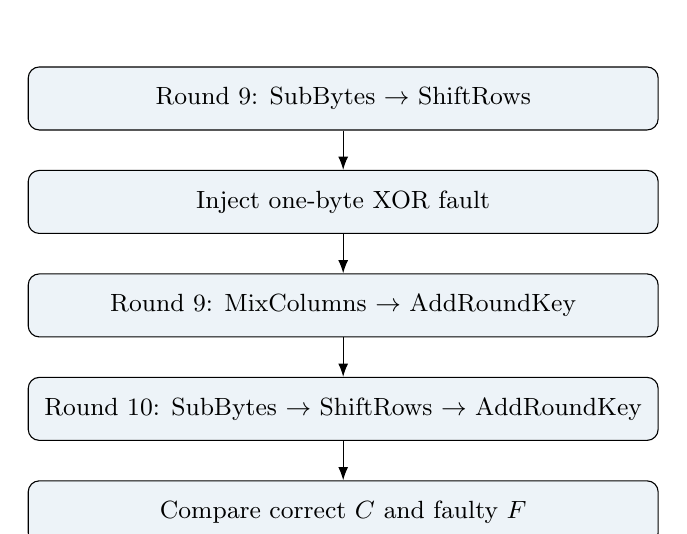
\begin{tikzpicture}[node distance=5mm, every node/.style={font=\small}, box/.style={draw,rounded corners,fill=pale,minimum width=8cm,minimum height=8mm},>=Latex]
\node[box] (a) {Round 9: SubBytes $\to$ ShiftRows};
\node[box,below=of a] (b) {Inject one-byte XOR fault};
\node[box,below=of b] (c) {Round 9: MixColumns $\to$ AddRoundKey};
\node[box,below=of c] (d) {Round 10: SubBytes $\to$ ShiftRows $\to$ AddRoundKey};
\node[box,below=of d] (e) {Compare correct $C$ and faulty $F$};
\foreach \x/\y in {a/b,b/c,c/d,d/e}{\draw[->] (\x)--(\y);}
\end{tikzpicture}\end{center}
\section{Propagation through MixColumns}
If the first byte of a column changes by \(e\), the column difference after MixColumns is
\[\Delta_{MC}=(02e,\ e,\ e,\ 03e)^T.\]
For \(e=\hex{01}\), this is \((\hex{02},\hex{01},\hex{01},\hex{03})^T\). AddRoundKey does not alter XOR differences because both executions use the same round key. The final SubBytes transforms these differences nonlinearly; ShiftRows moves them into separate ciphertext positions.
\section{Which ciphertext bytes are affected?}
For the four round-9 columns, the affected ciphertext positions (in corresponding row order) are:
\begin{center}\begin{tabular}{cc}\toprule Faulted column & Ciphertext byte positions\\\midrule 0&0, 13, 10, 7\\1&4, 1, 14, 11\\2&8, 5, 2, 15\\3&12, 9, 6, 3\\\bottomrule\end{tabular}\end{center}
\section{Constructing candidates for the last AES round key}
For an affected ciphertext position \(j\), and a guessed last-round key byte \(k\), compute
\[d_j(k)=S^{-1}(C_j\xor k)\xor S^{-1}(F_j\xor k).\]
Each byte has 256 candidate values. Four unknown key bytes have \(256^4=2^{32}\) possible combinations before filtering.
Construct a set \(\mathcal D\) containing the MixColumns output differences for a single nonzero faulty byte in any of the four row positions:
\[\mathcal D=\{M(e\mathbf e_r):r\in\{0,1,2,3\},\ e\in\{1,\ldots,255\}\}.\]
This produces \(4\cdot255=1020\) four-byte difference patterns (not 1020 individual bytes). For each proposed key quartet, compute the four \(d_j(k)\) values in their correct \emph{pre-ShiftRows row order} and keep the quartet only if the resulting vector lies in \(\mathcal D\).
\section{Intersecting observations}
A single correct/faulty pair typically leaves multiple candidate key quartets. Repeat with independent faults in the same column and intersect the candidate sets:
\[\mathcal K_{\mathrm{surviving}}=\mathcal K_1\cap\mathcal K_2\cap\cdots.\]
Repeat across all four columns to recover the full 16-byte \(K_{10}\). The notes illustrate candidate filtering using a hypothetical quartet \((\hex{13},\hex{2B},\hex{A7},\hex{17})\); such pedagogical candidate examples should not be confused with a complete independently verified AES fault trace.
\section{Two injection depths: round 9 versus round 8}
\label{sec:piret_two_models}
The same Piret principle can be applied at two different depths, and the project's
analysis distinguishes them because they behave very differently. The choice is
the \texttt{fault\_round} argument of the target in \texttt{piret\_aes.py}.

\begin{description}
\item[Round-9 model (one column group).] The fault is injected before the
round-9 MixColumns, as described above. MixColumns spreads the single faulted
byte over \emph{one} column (four bytes); ShiftRows then scatters those four
bytes to four ciphertext positions. One faulty ciphertext therefore constrains
only \emph{one} group of four last-round key bytes. To recover all sixteen bytes
of \(K_{10}\), the campaign must be repeated for each of the four columns.
\item[Round-8 model (all four groups at once).] The fault is injected one round
earlier, before the round-8 MixColumns. Now the difference passes through
\emph{two} MixColumns layers: round-8 MixColumns spreads the single byte to a
full column, and round-9 MixColumns spreads each of those bytes across all four
columns. Before the final round the difference already touches all sixteen state
bytes, so a single faulty ciphertext constrains \emph{all four} key-byte groups
simultaneously. This is why the measured campaigns recover the complete
last-round key from a median of only two faulty ciphertexts.
\end{description}

\noindent The trade-off is depth versus count: the round-8 model needs far fewer
faulty ciphertexts but assumes a cleaner, more deeply propagated fault and larger
per-observation candidate structures; the round-9 model is simpler to reason
about per column but must be repeated. The default command line and the analysis
use the round-8 model; \texttt{run.py} follows the round-9 model used in the
lecture notes. Both reduce to the same last-round key once enough observations
are intersected.

\section{Reversing AES-128 key expansion}
Let \(w_0,\ldots,w_{43}\) be 32-bit expanded-key words. For \(i\ge4\),
\[w_i=\begin{cases}w_{i-4}\xor g(w_{i-1}),&i\equiv0\pmod4,\\w_{i-4}\xor w_{i-1},&\text{otherwise},\end{cases}\]
where \(g(w)=\operatorname{SubWord}(\operatorname{RotWord}(w))\xor\operatorname{Rcon}\). In reverse, compute \(w_{i-4}\) by XORing \(w_i\) with the same known right-hand transformation. Begin with \(w_{40},\ldots,w_{43}\) from \(K_{10}\) and work backward to \(w_0,\ldots,w_3\), yielding \(K_0\). No inverse S-box is required for this reversal because the relevant inputs to \(g\) are already known.

\chapter{SM4: Complete Structure and First Round}
\section{Official test vector}
\begin{center}\begin{tabular}{ll}\toprule Plaintext&\hex{01234567\allowbreak{}89ABCDEF\allowbreak{}FEDCBA98\allowbreak{}76543210}\\Master key&\hex{01234567\allowbreak{}89ABCDEF\allowbreak{}FEDCBA98\allowbreak{}76543210}\\Ciphertext&\hex{681EDF34\allowbreak{}D206965E\allowbreak{}86B3E94F\allowbreak{}536E4246}\\\bottomrule\end{tabular}\end{center}
Split the plaintext into four 32-bit words:
\[X_0=\hex{01234567},\quad X_1=\hex{89ABCDEF},\quad X_2=\hex{FEDCBA98},\quad X_3=\hex{76543210}.\]
\section{SM4 round function}
SM4 performs 32 rounds, producing one new 32-bit word per round:
\[\boxed{X_{i+4}=X_i\xor T(X_{i+1}\xor X_{i+2}\xor X_{i+3}\xor rk_i)}.\]
Write \(T=L\circ\tau\), where \(\tau\) substitutes the four bytes through the SM4 S-box and
\[L(B)=B\xor(B\rol2)\xor(B\rol10)\xor(B\rol18)\xor(B\rol24).\]
The output reverses the final four words:
\[C=X_{35}\parallel X_{34}\parallel X_{33}\parallel X_{32}.\]
\section{SM4 key expansion}
The four initial key-schedule words are \(K_i=MK_i\xor FK_i\), with
\[\begin{array}{ll}FK_0=\hex{A3B1BAC6},&FK_1=\hex{56AA3350},\\FK_2=\hex{677D9197},&FK_3=\hex{B27022DC}.\end{array}\]
The key-schedule recurrence is
\[K_{i+4}=K_i\xor T'(K_{i+1}\xor K_{i+2}\xor K_{i+3}\xor CK_i),\quad rk_i=K_{i+4},\]
with \(T'=L'\circ\tau\) and
\[L'(B)=B\xor(B\rol13)\xor(B\rol23).\]
\textbf{Crucial distinction:} encryption uses \(L\), while key expansion uses \(L'\). They have different rotation constants.
For the first round, \(rk_0=\hex{F12186F9}\).
\section{Detailed computation of encryption round 0}
\paragraph{Step 1: XOR the three newest words with the round key.}
\[A=X_1\xor X_2\xor X_3\xor rk_0=\hex{F002C39E}.\]
\paragraph{Step 2: Apply the SM4 S-box to each byte.}
\[\hex{F0}\mapsto\hex{18},\quad\hex{02}\mapsto\hex{E9},\quad\hex{C3}\mapsto\hex{92},\quad\hex{9E}\mapsto\hex{B1}.\]
Thus \(B=\tau(A)=\hex{18E992B1}\).
\paragraph{Step 3: Apply the linear transformation.}
\begin{center}\begin{tabular}{ll}\toprule Term&Hexadecimal value\\\midrule\(B\)&\hex{18E992B1}\\\(B\rol2\)&\hex{63A64AC4}\\\(B\rol10\)&\hex{A64AC463}\\\(B\rol18\)&\hex{4AC463A6}\\\(B\rol24\)&\hex{B118E992}\\\midrule XOR of all five&\hex{26D99622}\\\bottomrule\end{tabular}\end{center}
\paragraph{Step 4: XOR with the oldest word.}
\[X_4=X_0\xor L(B)=\hex{01234567}\xor\hex{26D99622}=\boxed{\hex{27FAD345}}.\]
The next four-word window is \((X_1,X_2,X_3,X_4)\). The following words are \(X_5=\hex{A18B4CB2}\), \(X_6=\hex{11C1E22A}\), and \(X_7=\hex{CC13E2EE}\). After 32 rounds and the output reversal, the official ciphertext is obtained.

\chapter{Differential Fault Analysis of SM4: A Worked Last-Round Model}
\section{Attack model and limitations}
We use a \emph{controlled, known XOR fault} in one byte of the input to the SM4 S-boxes in round 31. This is a pedagogical model, not a claim that a real clock/voltage glitch yields a known XOR value. In this model, all other round inputs remain unchanged.
The last round is
\[X_{35}=X_{31}\xor L(\tau(A)),\qquad A=X_{32}\xor X_{33}\xor X_{34}\xor rk_{31}.\]
The attacker observes the correct ciphertext and a faulty ciphertext. The secret internal values below are supplied \emph{only for checking the simulation}.
\section{Known ciphertext and hidden internal values}
\[\begin{array}{ll}X_{35}=\hex{681EDF34},&X_{34}=\hex{D206965E},\\X_{33}=\hex{86B3E94F},&X_{32}=\hex{536E4246}.\end{array}\]
For this official test vector, the simulation has
\[X_{31}=\hex{7B938F4C},\quad A=\hex{96FF9D45},\quad rk_{31}=\hex{9124A012}.\]
The attacker must recover the key rather than assume it.
\section{Step 1: Inject a known XOR fault}
Alter the first byte of \(A\) by \(e=\hex{01}\):
\[A=\hex{96FF9D45}\longrightarrow A'=\hex{97FF9D45}.\]
\section{Step 2: Observe the S-box difference}
The two S-box outputs are
\[B=\tau(A)=\hex{1A488C73},\qquad B'=\tau(A')=\hex{55488C73}.\]
Consequently,
\[\Delta B=B\xor B'=\hex{4F000000}.\]
\section{Step 3: Propagate the difference through L}
Because \(L\) is XOR-linear,
\[\Delta X_{35}=L(B)\xor L(B')=L(\Delta B)=\hex{734E3D3D}.\]
The correct last word is \(X_{35}=\hex{681EDF34}\), so the faulty last word is
\[X'_{35}=\hex{681EDF34}\xor\hex{734E3D3D}=\hex{1B50E209}.\]
Therefore the attacker sees
\begin{center}\begin{tabular}{ll}\toprule Correct ciphertext&\hex{681EDF34 D206965E 86B3E94F 536E4246}\\Faulty ciphertext&\hex{1B50E209 D206965E 86B3E94F 536E4246}\\Difference&\hex{734E3D3D 00000000 00000000 00000000}\\\bottomrule\end{tabular}\end{center}
\section{Step 4: Undo the linear layer from observed data}
The attacker computes
\[\Delta B=L^{-1}(\Delta X_{35})=L^{-1}(\hex{734E3D3D})=\hex{4F000000}.\]
The first S-box byte therefore satisfies
\[S(a)\xor S(a\xor\hex{01})=\hex{4F}.\]
Enumerating all 256 possible input bytes gives the candidate set
\[\mathcal A_1=\{\hex{96},\hex{97}\}.\]
\section{Step 5: Convert S-box input candidates to key candidates}
The attacker knows the last three words from the ciphertext:
\[X_{32}\xor X_{33}\xor X_{34}=\hex{07DB3D57}.\]
Since \(rk_{31}=A\xor\hex{07DB3D57}\), the first byte of the key is
\[rk_{31}[0]=a\xor\hex{07}.\]
Thus \(a=\hex{96}\) yields \(\hex{91}\), while \(a=\hex{97}\) yields \(\hex{90}\). After one observation, the candidates are \(\{\hex{91},\hex{90}\}\).
\section{Step 6: Use independent observations}
Repeat with the \emph{same plaintext and state}, but use a known XOR fault \(e=\hex{02}\). The new S-box difference is \(d_2=\hex{81}\). Keep only input candidates satisfying both
\[\begin{cases}S(a)\xor S(a\xor\hex{01})=\hex{4F},\\S(a)\xor S(a\xor\hex{02})=\hex{81}.\end{cases}\]
The intersection identifies \(a=\hex{96}\), hence \(rk_{31}[0]=\hex{91}\).
\section{Step 7: Repeat for the other three bytes}
The supplied worked example reports the following bytewise observations under the same controlled-fault assumption:
\begin{center}\begin{tabular}{ccccc}\toprule Byte&\(d\) for \(e=01\)&\(d\) for \(e=02\)&Recovered \(A\)&Recovered \(rk_{31}\)\\\midrule0&4F&81&96&91\\1&71&83&FF&24\\2&79&6F&9D&A0\\3&80&C9&45&12\\\bottomrule\end{tabular}\end{center}
This reconstructs
\[A=\hex{96FF9D45},\qquad rk_{31}=A\xor\hex{07DB3D57}=\boxed{\hex{9124A012}}.\]
\note{This illustrates last-round subkey recovery \emph{conditional on the fault model}. The listed observations should be validated against a software implementation before treating them as experimental results.}
\section{What happens after recovering the last subkey?}
Knowing \(rk_{31}\), reconstruct the previous state word:
\[X_{31}=X_{35}\xor T(X_{32}\xor X_{33}\xor X_{34}\xor rk_{31}).\]
For the example, \(X_{31}=\hex{7B938F4C}\). However, this does \emph{not} automatically reveal \(rk_{30}\). Additional fault observations and state constraints are required for rounds 30, 29, and 28. The present worked example does not demonstrate that stage of the attack.

\chapter{SM4 DFA: How the Calculations Work}
\label{chap:complete_calculations}
This chapter explains the method with short numerical examples. Repeated matrix
operations, exhaustive candidate lists and the 32 individual reverse-schedule
steps are omitted; the same rules apply to each remaining bit, byte or round.

\section{Undoing the linear transformation}
For an isolated last-round fault, XOR cancels the unchanged older state word:
\[
\Delta X_{35}=L(B)\xor L(B')=L(B\xor B')=L(\Delta B).
\]
Therefore the attacker needs $\Delta B=L^{-1}(\Delta X_{35})$. This operation
uses only the public SM4 transformation, not the secret key.

The data diffusion map is
\[
L(B)=B\xor(B\rol2)\xor(B\rol10)\xor(B\rol18)\xor(B\rol24).
\]
For example, $B=\hex{4F000000}$ gives $L(B)=\hex{734E3D3D}$.
The inverse restores the localized S-box output difference:
\[
L^{-1}(\hex{734E3D3D})=\boxed{\hex{4F000000}}.
\]
The nonzero first byte is $\hex{4F}$. Several changed ciphertext bytes can
therefore originate from one affected S-box byte.

\section{How the inverse matrix is obtained}
Each 32-bit word is a vector of 32 bits. Since XOR and fixed rotations are
linear over GF(2), $L$ has a binary $32\times32$ matrix $M$.
Apply $L$ to each basis word $2^i$: the result supplies column $i$ of $M$.
For example,
\[
L(\hex{00000001})=\hex{01040405}.
\]
To invert $M$, augment it with the identity and perform Gaussian elimination:
\[
[M\mid I]\ \longrightarrow\ [I\mid M^{-1}].
\]
For each column, choose a row containing a 1 as the pivot, swap it into place,
and XOR it into every other row containing a 1 in that column. Over GF(2),
subtraction is XOR; no division is needed because the only nonzero pivot is 1.
The function \texttt{inverse\_rows()} prepares these inverse rows once and
caches them. It does not process a particular ciphertext difference.

\section{How the inverse is applied to a value}
The function \texttt{inverse\_linear(value)} uses those rows to compute the
32 result bits. For inverse row $r_j$ and input $d$:
\[
t_j=r_j\mathbin{\&}d,\qquad
b_j=\operatorname{popcount}(t_j)\bmod2.
\]
AND selects the input bits that participate in this output bit. Their XOR is
their parity: an odd number of ones gives 1; an even number gives 0.
For example, using $d=\hex{734E3D3D}$ and the first inverse row:
\[
\hex{51154505}\mathbin{\&}\hex{734E3D3D}=\hex{51040505}.
\]
There are eight set bits, so result bit 0 is $8\bmod2=0$.
Repeating this for the other rows and placing each bit at its index produces
$\hex{4F000000}$. Bit index 0 means the least significant bit, whereas byte
index 0 in the attack means the most significant byte.

\section{From a difference to a subkey byte}
For a known error mask $e$, test all 256 possible S-box inputs $a$ against
\[
S(a)\xor S(a\xor e)=d.
\]
In the worked example, $e_1=\hex{01}$ and $d_1=\hex{4F}$ leave
$\mathcal A_1=\{\hex{96},\hex{97}\}$. A second observation,
$e_2=\hex{02}$ and $d_2=\hex{81}$, leaves
$\mathcal A_2=\{\hex{75},\hex{77},\hex{94},\hex{96}\}$.
Their intersection is $\{\hex{96}\}$.

The three unchanged ciphertext words provide
\[
q=\operatorname{byte}_0(\hex{D206965E}\xor\hex{86B3E94F}
\xor\hex{536E4246})=\hex{07}.
\]
Since $a=q\xor rk_{31}[0]$, the recovered byte is
\[
rk_{31}[0]=\hex{96}\xor\hex{07}=\boxed{\hex{91}}.
\]
The other three bytes follow the same procedure. A byte is accepted only when
its candidate intersection is unique. The unknown-bit Giraud-inspired variant
instead accepts any of the eight one-bit masks for each observation, which can
leave more candidates; Section~\ref{sec:four_sm4_configurations} defines all four
experimental configurations.

\section{Recovering earlier subkeys and the master key}
After recovering $rk_{31}$, undo that round using
\[
X_{31}=X_{35}\xor
L\bigl(\tau(X_{32}\xor X_{33}\xor X_{34}\xor rk_{31})\bigr).
\]
Apply this reconstruction to both clean and faulty ciphertexts. New faults
targeting round 30 then reveal $rk_{30}$ using the same byte filter. Repeat
for rounds 29 and 28, always peeling only rounds whose keys are already known.
One recovered 32-bit subkey does not reveal the complete 128-bit master key.

With four consecutive subkeys, reverse the schedule by XORing the known
transformed term back out:
\[
K_i=K_{i+4}\xor T'(K_{i+1}\xor K_{i+2}\xor K_{i+3}\xor CK_i).
\]
For instance, $K_{32},K_{33},K_{34},K_{35}$ are respectively
$\hex{428D3654}$, $\hex{62293496}$, $\hex{01CF72E5}$ and $\hex{9124A012}$.
Using the public constant $CK_{31}=\hex{646B7279}$ yields
$K_{31}=\hex{F1780C81}$. Here $T'=L'\circ\tau$, with
$L'(Z)=Z\xor(Z\rol13)\xor(Z\rol23)$; its rotations differ from those of $L$.
Continue down to $K_0,\ldots,K_3$, remove the fixed constants
$MK_i=K_i\xor FK_i$, and concatenate the four words.
The example yields $MK=\hex{0123456789ABCDEFFEDCBA9876543210}$.
Finally, regenerate the subkeys and check encryption and decryption with the
recovered key.

\chapter{SM4: Recovering the Master Key from Four Round Keys}
\section{Required subkeys}
If four consecutive final subkeys have been recovered, then
\begin{center}\begin{tabular}{cc}\toprule Key-schedule word&Round key\\\midrule\(K_{32}\)&\(rk_{28}=\hex{428D3654}\)\\\(K_{33}\)&\(rk_{29}=\hex{62293496}\)\\\(K_{34}\)&\(rk_{30}=\hex{01CF72E5}\)\\\(K_{35}\)&\(rk_{31}=\hex{9124A012}\)\\\bottomrule\end{tabular}\end{center}
These are reference subkeys from the official example; \emph{only} \(rk_{31}\) was recovered in the preceding pedagogical DFA walkthrough. the attack walkthrough in Part 2 explains how the current code actually recovers all four subkeys with a selectable-round fault oracle.
\section{Reverse the recurrence}
The forward key schedule is
\[K_{i+4}=K_i\xor T'(K_{i+1}\xor K_{i+2}\xor K_{i+3}\xor CK_i).\]
XOR is self-inverse, so
\[\boxed{K_i=K_{i+4}\xor T'(K_{i+1}\xor K_{i+2}\xor K_{i+3}\xor CK_i)}.\]
Start with \(i=31\), then decrease to \(i=0\). For example,
\[K_{31}=K_{35}\xor T'(K_{32}\xor K_{33}\xor K_{34}\xor CK_{31}),\]
where \(CK_{31}=\hex{646B7279}\). This yields the previous expanded-key word \(K_{31}=\hex{F1780C81}\) in the official test vector. Continue to recover \(K_0,K_1,K_2,K_3\).
\section{Undo the initial constants}
Finally,
\[MK_i=K_i\xor FK_i\qquad(i=0,1,2,3),\]
and concatenate the four master-key words:
\[\boxed{MK=\hex{01234567\allowbreak{}89ABCDEF\allowbreak{}FEDCBA98\allowbreak{}76543210}}.\]

\chapter{Giraud Fault Attack on AES-128 and Its Adaptation to SM4}
\label{chap:giraud}
\section{Core idea and comparison with Piret--Quisquater}
Giraud's AES fault-analysis approach exploits a \emph{single-bit} fault close to the last round. In contrast to the Piret--Quisquater example, which injects a byte fault before the ninth-round MixColumns and typically modifies four ciphertext bytes, a single-byte fault immediately before the final SubBytes affects only one ciphertext byte: the last AES round does not contain MixColumns. The attacker tests last-round key-byte candidates by checking whether the inverse-S-box input difference has Hamming weight one.

\section{AES-128: precise fault location}
Let $U$ denote the state after round 9 AddRoundKey, just before round 10 SubBytes. A one-bit XOR fault modifies a single input byte $a$ into $a'=a\xor e$, where $e\in\{\hex{01},\hex{02},\hex{04},\hex{08},\hex{10},\hex{20},\hex{40},\hex{80}\}$. Round 10 performs SubBytes, ShiftRows and AddRoundKey $K_{10}$; there is no MixColumns. ShiftRows relocates the changed byte without increasing the number of affected bytes.

For the affected ciphertext position $j$, with correct byte $c$, faulty byte $f$, and unknown last-round key byte $k$, the attacker evaluates
\begin{equation}
\delta(k)=S_{\mathrm{AES}}^{-1}(c\xor k)\xor S_{\mathrm{AES}}^{-1}(f\xor k).
\label{eq:giraud_aes_test}
\end{equation}
The candidate is compatible with the fault model if
\begin{equation}
\delta(k)\in\mathcal E=\{\hex{01},\hex{02},\hex{04},\hex{08},\hex{10},\hex{20},\hex{40},\hex{80}\}.
\end{equation}
Equivalently, the 8-bit value $\delta(k)$ must have Hamming weight exactly one. If the injected bit position is known, the condition can be made stronger: $\delta(k)=e$.

\section{Worked AES-128 example: the first ciphertext byte}
We use the official AES-128 test vector already introduced in this report:
\begin{align*}
P&=\hex{00112233\allowbreak{}44556677\allowbreak{}8899AABB\allowbreak{}CCDDEEFF},\\
K_0&=\hex{00010203\allowbreak{}04050607\allowbreak{}08090A0B\allowbreak{}0C0D0E0F},\\
C&=\hex{69C4E0D8\allowbreak{}6A7B0430\allowbreak{}D8CDB780\allowbreak{}70B4C55A}.
\end{align*}
The first byte entering the final SubBytes is $a=\hex{BD}$. Inject $e=\hex{01}$ in that byte:
\begin{equation}
\hex{BD}\xor\hex{01}=\hex{BC}.
\end{equation}
The AES S-box maps $S(\hex{BD})=\hex{7A}$ and $S(\hex{BC})=\hex{65}$. The first byte of $K_{10}$ is $\hex{13}$, so
\begin{align*}
c&=\hex{7A}\xor\hex{13}=\hex{69},\\
f_1&=\hex{65}\xor\hex{13}=\hex{76}.
\end{align*}
Thus the simulated faulty ciphertext is
\begin{equation}
F_1=\hex{76C4E0D8\allowbreak{}6A7B0430\allowbreak{}D8CDB780\allowbreak{}70B4C55A}.
\end{equation}
The attacker does not assume the value $\hex{13}$: it is shown here solely to verify the example. For candidate $k=\hex{13}$, equation~\eqref{eq:giraud_aes_test} gives
\begin{align*}
S^{-1}(\hex{69}\xor\hex{13})&=S^{-1}(\hex{7A})=\hex{BD},\\
S^{-1}(\hex{76}\xor\hex{13})&=S^{-1}(\hex{65})=\hex{BC},\\
\delta(\hex{13})&=\hex{BD}\xor\hex{BC}=\boxed{\hex{01}}.
\end{align*}
The candidate is compatible with a single-bit fault, but one correct/faulty pair may leave several candidates.

\section{Multiple faults and candidate intersection}
Repeat the encryption with the same plaintext and key and introduce an independent single-bit fault at the same location. In the worked example, choosing $e_2=\hex{02}$ produces $a_2'=\hex{BF}$ and a second faulty first ciphertext byte $f_2=\hex{1B}$. For observation $t$, define
\begin{equation}
\mathcal K_t=\bigl\{k\in\{0,\ldots,255\}:S^{-1}(c\xor k)\xor S^{-1}(f_t\xor k)\in\mathcal E\bigr\}.
\end{equation}
The surviving candidates are the intersection $\mathcal K=\bigcap_t\mathcal K_t$. For the illustrated pair of faults, the recovered first byte is $K_{10}[0]=\hex{13}$. The number of observations required is not fixed: it depends on the fault model and the observed differences.

Repeating the experiment across all sixteen pre-final-SubBytes byte positions allows the attacker, under this model, to reconstruct all sixteen bytes of $K_{10}$. For the official vector,
\begin{equation}
K_{10}=\hex{13111D7F\allowbreak{}E3944A17\allowbreak{}F307A78B\allowbreak{}4D2B30C5}.
\end{equation}
The AES-128 key schedule can then be reversed to recover the original key $K_0$, as explained in the preceding AES key-expansion chapter.

\section{Adaptation of the single-bit idea to SM4}
\label{sec:giraud_sm4}
The corresponding SM4 experiment is an \emph{adaptation of the single-bit differential filtering principle}, rather than a claim that the original AES attack transfers unchanged. The SM4 last round is
\begin{equation}
X_{35}=X_{31}\xor L\bigl(\tau(A)\bigr),\qquad A=X_{32}\xor X_{33}\xor X_{34}\xor rk_{31}.
\end{equation}
The output is $C=(X_{35},X_{34},X_{33},X_{32})$. Inject a single-bit fault in one byte of $A$, just before the last-round S-boxes. Unlike AES, the SM4 linear map $L$ diffuses the one-byte S-box output difference over the 32-bit word $X_{35}$. The other three ciphertext words remain unchanged \emph{under the assumed isolated-fault model}.

Let $F$ be the faulty ciphertext and $\Delta X_{35}=X_{35}\xor X'_{35}$. Since $L$ is linear and invertible, the attacker can compute
\begin{equation}
\Delta B=L^{-1}(\Delta X_{35})=\tau(A)\xor\tau(A').
\end{equation}
For an affected byte with S-box input $a$ and unknown single-bit error $e$, candidate inputs satisfy
\begin{equation}
S_{\mathrm{SM4}}(a)\xor S_{\mathrm{SM4}}(a\xor e)=d,
\quad e\in\mathcal E,
\end{equation}
where $d$ is the corresponding byte of $\Delta B$. If $e$ is known from the simulation, it is used directly; otherwise all eight one-bit masks must be tested. Multiple correct/faulty observations reduce the candidate set by intersection.

\section{Worked SM4 example and recovery of \texorpdfstring{$rk_{31}$}{rk31}}
Using the official SM4 test vector,
\begin{align*}
P&=\hex{01234567\allowbreak{}89ABCDEF\allowbreak{}FEDCBA98\allowbreak{}76543210},\\
MK&=\hex{01234567\allowbreak{}89ABCDEF\allowbreak{}FEDCBA98\allowbreak{}76543210},\\
C&=\hex{681EDF34\allowbreak{}D206965E\allowbreak{}86B3E94F\allowbreak{}536E4246},
\end{align*}
the simulated input of the last S-box layer is $A=\hex{96FF9D45}$. A one-bit fault $e=\hex{01000000}$ gives $A'=\hex{97FF9D45}$. The substitution outputs are
\begin{align*}
\tau(A)&=\hex{1A488C73},\\
\tau(A')&=\hex{55488C73},\\
\Delta B&=\hex{4F000000}.
\end{align*}
After the linear layer,
\begin{equation}
\Delta X_{35}=L(\hex{4F000000})=\hex{734E3D3D}.
\end{equation}
Therefore the faulty output is
\begin{equation}
F_1=\hex{1B50E209\allowbreak{}D206965E\allowbreak{}86B3E94F\allowbreak{}536E4246}.
\end{equation}
From the observed difference alone, the attacker obtains $\Delta B=L^{-1}(\hex{734E3D3D})=\hex{4F000000}$. With known fault mask $\hex{01}$ in the first byte, the candidate equation is
\begin{equation}
S_{\mathrm{SM4}}(a)\xor S_{\mathrm{SM4}}(a\xor\hex{01})=\hex{4F}.
\end{equation}
The first observation permits $a\in\{\hex{96},\hex{97}\}$. A second simulated fault of mask $\hex{02}$ gives the first-byte S-box difference $\hex{81}$. Intersecting both sets identifies $a=\hex{96}$.

The three known ciphertext words yield
\begin{equation}
X_{32}\xor X_{33}\xor X_{34}=\hex{07DB3D57}.
\end{equation}
Thus the first last-round key byte is
\begin{equation}
rk_{31}[0]=\hex{96}\xor\hex{07}=\boxed{\hex{91}}.
\end{equation}
The supplied worked example applies analogous observations to the remaining three S-box inputs, obtaining
\begin{equation}
A=\hex{96FF9D45},\qquad rk_{31}=A\xor\hex{07DB3D57}=\boxed{\hex{9124A012}}.
\end{equation}
The bytewise simulated differences are summarized below.
\begin{center}
\begin{tabular}{ccccc}\toprule
Byte&$d$ for $e=01$&$d$ for $e=02$&Recovered $A$&Recovered $rk_{31}$\\\midrule
0&4F&81&96&91\\
1&71&83&FF&24\\
2&79&6F&9D&A0\\
3&80&C9&45&12\\\bottomrule
\end{tabular}
\end{center}
\note{The numerical values in this subsection are simulated, not physical fault-injection measurements. In particular, knowledge of the exact XOR mask is a strong experimental assumption.}

\section{From the final SM4 subkey to the master key}
Recovering $rk_{31}$ is not equivalent to recovering the 128-bit master key. The SM4 key schedule needs four consecutive 32-bit round keys to be inverted. In the official test vector these are
\begin{align*}
rk_{28}&=\hex{428D3654},&rk_{29}&=\hex{62293496},\\
rk_{30}&=\hex{01CF72E5},&rk_{31}&=\hex{9124A012}.
\end{align*}
The values $rk_{28}$, $rk_{29}$ and $rk_{30}$ are \emph{reference values}, not keys shown to have been recovered by the two last-round faults. The two last-round faults do not recover these other keys. The implemented multi-round extension in the attack walkthrough in Part 2 obtains them by requesting new faults in rounds 30, 29 and 28 and undoing previously recovered later rounds.

With four consecutive round keys, set $K_{i+4}=rk_i$ and invert the SM4 recurrence:
\begin{equation}
K_i=K_{i+4}\xor T'\bigl(K_{i+1}\xor K_{i+2}\xor K_{i+3}\xor CK_i\bigr).
\end{equation}
Iterating backward yields $K_0,K_1,K_2,K_3$. Undo the fixed initial constants $FK_i$ via $MK_i=K_i\xor FK_i$ and concatenate the four words to recover the 128-bit master key.

\section{Experimental implications}
A software simulation can inject an exact XOR mask at a chosen intermediate value. On an STM32 target, a voltage or clock glitch may instead alter multiple bits, skip an instruction, affect control flow, or produce no useful fault. A practical evaluation should therefore log correct and faulty ciphertexts, classify observed fault patterns, verify whether the assumed location and single-bit model are plausible, and report recovery success separately from simulation-only results.

\chapter{Causing Single-Bit Faults in Practice}
\label{chap:physical_faults}

The attacks in this report assume a very specific event: a short, transient fault
that changes one bit (Giraud) or one byte (Piret) of an intermediate value, at a
chosen instruction, while leaving everything else correct. The mathematics then
turns the correct/faulty ciphertext pair into key information. This chapter
explains, at the level of a laboratory evaluation, how such faults are produced
on real hardware, how far the clean single-bit model is from typical practice,
and which countermeasures remove the attacker's advantage. It is written for a
defensive security evaluation on the project's own ChipWhisperer target; it is
not a procedure against any third-party device.

\section{Why a physical fault appears}
Digital logic is correct only when every signal settles within one clock period
and every transistor is powered within its specified range. A fault-injection
technique deliberately violates one of these guarantees for a very short time, so
that a flip-flop latches a value that has not finished computing, or a memory
cell flips. Because the violation is brief and localised, most of the
computation stays correct and only a few bits are disturbed --- which is exactly
what differential fault analysis needs.

\section{Common injection techniques}
\begin{description}
\item[Clock glitching.] When the attacker controls the device clock, inserting
one abnormally short clock period forces a register to sample before the slowest
combinational path has settled. The bits on the slow paths latch incorrectly.
The resulting fault depends on the implementation and timing. In the
ChipWhisperer-Lite setup, clock injection requires an accessible target clock
path. No single-bit accuracy or completed physical STM32 campaign is established
by the software experiments in this report.
\item[Voltage glitching.] A brief, sharp drop (or spike) on the supply rail slows
gate switching so that, again, logic fails to settle in time. It needs no clock
access and little equipment --- a transistor pulling the rail low (a ``crowbar'')
is enough --- which makes it one of the most widely used techniques. Its spatial
and bit-level precision depends on the target and experimental arrangement;
neither method guarantees a selected bit flip.
\item[Electromagnetic (EM) pulse injection.] A small coil held over the package
emits a fast magnetic pulse that induces transient currents in nearby logic. It
is contactless, needs no decapsulation, and can be aimed at a region of the die,
giving some spatial selectivity.
\item[Optical / laser injection.] A focused light or laser pulse on an exposed
(decapsulated) die deposits charge in specific cells. It is the most precise
technique and can come closest to a true, chosen single-bit fault, but it is
invasive and requires expensive equipment and sample preparation.
\item[Auxiliary stressors.] Temperature and body-biasing shift timing margins and
are sometimes combined with the above to widen the window in which a glitch
succeeds.
\end{description}

\section{Hitting the right instruction}
Producing a disturbance is only half the problem; it must land on the targeted
operation (for Giraud, the byte just before the final SubBytes). Two controls do
this:
\begin{itemize}
\item A \textbf{trigger} marks when the sensitive computation runs. In this
project the firmware raises a GPIO line (TIO4) around the cipher, and the capture
hardware watches it. A real evaluation may instead trigger on a power or EM
feature.
\item A \textbf{delay} after the trigger selects \emph{which} clock cycle, and
therefore which instruction, receives the glitch; the glitch \emph{width} and
\emph{offset} set its strength. An evaluation sweeps these parameters, repeats
each setting many times, and classifies the outcome.
\end{itemize}

\section{The gap between the model and reality}
A real campaign does not produce clean single-bit faults on demand. Each attempt
typically falls into one of several outcomes:
\begin{center}
\begin{tabular}{ll}\toprule
Observed outcome & Use for DFA \\\midrule
No effect (correct output) & none \\
Reset or crash & none \\
Instruction skip / control-flow change & different attack class \\
Multi-bit or multi-byte fault & usually breaks the single-fault model \\
Clean one-bit / one-byte transient fault & \emph{this} is what Giraud/Piret need \\\bottomrule
\end{tabular}
\end{center}
\noindent The clean case is often a minority of attempts. The practical workflow
is therefore statistical: log the correct ciphertext and every faulty ciphertext
with its glitch parameters, \emph{filter} for the faults whose difference matches
the assumed model, and feed only those to the solver. This is why the software
experiments in this report separate the target (which may expose internal state)
from the solver (which sees only ciphertexts): the solver is written to accept
exactly the observations a real, filtered campaign would yield.

\note{The numerical examples elsewhere in this report inject an exact XOR in
software, so the fault model holds by construction. On the physical STM32 target
the same model must be \emph{established experimentally}: knowledge of the exact
bit (the \texttt{Giraud-known} variant) is a strong assumption that a campaign has
to justify by characterising its own glitches.}

\section{A taxonomy of fault widths and their consequences}
\label{sec:fault_taxonomy}
A disturbed computation can land anywhere on a spectrum, from no effect to a
corrupted whole word. What decides whether Giraud or Piret can use it is, above
all, the \emph{width} of the fault --- how many bits or bytes actually changed.
The two attacks are defined by the width they expect:
\begin{itemize}
\item \textbf{Giraud} expects \emph{exactly one bit} flipped at the input of the
last S-box layer.
\item \textbf{Piret} expects \emph{exactly one byte} corrupted (any nonzero
value) before the round-9 MixColumns.
\end{itemize}

\paragraph{Consequence by fault width.}
This is the dimension that decides whether an attack \emph{works} or \emph{breaks}.
\begin{center}
\begin{tabular}{P{.26\linewidth}P{.33\linewidth}P{.33\linewidth}}\toprule
Fault width & Giraud (model: 1 bit) & Piret (model: 1 byte) \\\midrule
Zero bits (no effect) & \(C=C'\), useless & \(C=C'\), useless \\
One bit & \emph{ideal} & works --- one bit is a byte of Hamming weight one \\
2--8 bits in the \textbf{same} byte & breaks: input difference has weight \(>1\), the weight-one filter rejects the true key & \emph{ideal} --- this is exactly a single-byte fault \\
One whole byte & breaks (same reason) & \emph{ideal} \\
\(\ge 2\) different state bytes & breaks the single-fault model & breaks: pattern no longer matches one byte in a column \\\bottomrule
\end{tabular}
\end{center}
\noindent The central observation is that \textbf{Piret is a superset of Giraud}:
every one-bit fault is also a one-byte fault (a byte value of Hamming weight one),
so the Piret solver accepts a bit, whereas Giraud demands weight one and rejects
anything wider. This is why, on SM4, the two attacks nearly coincide --- the only
difference is that Giraud assumes \(e\) is a single bit while Piret accepts the
whole byte.

\paragraph{Consequence by fault position (unknown location).}
Not knowing \emph{where} the fault landed does \emph{not} break the attack; it is
recovered by observation and raises the cost.
\begin{center}
\begin{tabular}{P{.3\linewidth}P{.36\linewidth}P{.26\linewidth}}\toprule
Situation & How it is resolved & Consequence \\\midrule
Unknown which column / key group & the set of changed ciphertext positions is the signature (see the column\(\to\)positions table of the Piret chapter) & none --- the group is \emph{read} from \(C\xor C'\) \\
Unknown exact position within the group & the solver sweeps all rows: \(\mathcal D=\{M(e\,\mathbf e_r):r\in\{0,1,2,3\},\,e\in\{1,\ldots,255\}\}\) & weaker filter \(\Rightarrow\) more faults \\\bottomrule
\end{tabular}
\end{center}
\noindent For AES Giraud this is even more direct: a one-bit fault changes exactly
one ciphertext byte (no MixColumns in the last round), so the changed position
already names the attacked key byte.

\paragraph{Consequence by fault value (unknown pattern).}
Not knowing the exact value does not break the attack either; it only weakens the
filter.
\begin{center}
\begin{tabular}{P{.16\linewidth}P{.27\linewidth}P{.27\linewidth}P{.14\linewidth}}\toprule
Attack & Value known & Value unknown & Measured \\\midrule
SM4 Giraud & exact bit: one mask & unknown bit: eight masks & median 32 versus 35 \\
AES Piret & \multicolumn{2}{P{.54\linewidth}}{The AES differential model can enumerate unknown nonzero byte errors.} & model dependent \\
SM4 controlled DFA & exact byte mask & not implemented by this known-mask filter & no claim \\\bottomrule
\end{tabular}
\end{center}
\noindent Distinguish the AES model from the project's SM4 controlled DFA:
the latter needs the exact error mask. The two plotted SM4 Piret configurations
change the ordered masks, not whether their values are known. Hiding an arbitrary
byte error would require a different filter and a new experimental evaluation.

\paragraph{Consequence by timing (wrong round or instruction).}
If the glitch lands on the wrong round or instruction, the difference propagates
through a different number of S-box layers and the pattern of changed bytes no
longer matches the expected one:
\begin{itemize}
\item Too early $\Rightarrow$ extra S-box layers scramble the difference $\Rightarrow$ matches no pattern $\Rightarrow$ filtered out.
\item Too late (e.g.\ already at the output) $\Rightarrow$ wrong positions change $\Rightarrow$ filtered out.
\end{itemize}
The delay sweep of \S\ref{sec:fault_taxonomy}'s sibling section exists precisely
to place the glitch on the right cycle.

\paragraph{Summary.}
\begin{center}
\begin{tabular}{P{.32\linewidth}P{.17\linewidth}P{.15\linewidth}P{.2\linewidth}}\toprule
What you do not know / what happened & Giraud & Piret & Action \\\midrule
No effect & useless & useless & discard \\
One bit, bit known & \checkmark\ 32 faults & \checkmark\ works & solve \\
One bit, bit unknown & \checkmark\ \({\approx}34.6\) & \checkmark\ works & sweep \(e\) \\
Several bits, same byte & breaks & \checkmark\ ideal & Piret solver \\
One byte, pos.\ unknown & n/a & \checkmark\ more faults & read group, sweep \(r\) \\
Several bytes & breaks & breaks & discard \\
Wrong round / instr. & no match & no match & retune delay \\\bottomrule
\end{tabular}
\end{center}
\noindent The rule that ties it together: the less you know (value, position), the
\emph{weaker the filter} and the \emph{more faults} you need --- but the attack
stays valid. What actually \emph{breaks} an attack is the width leaving the model:
more than one byte breaks both, while more than one bit breaks only Giraud (Piret
still holds).

\section{How can one bit actually be changed?}
In the simulator, $a'=a\xor2^j$ explicitly flips bit $j$. On the STM32F303,
the host generally cannot command ``flip this internal bit'' through the
ChipWhisperer-Lite. Its clock and voltage pulse generators perturb physical
conditions. A selected timing window may produce no change, a reset, an
instruction fault, or a data error of varying width. Laser and EM injection
require additional equipment; spatial targeting still does not by itself prove
that exactly one desired algorithmic bit was flipped.

For a diagnostic firmware build on the laboratory target, compare the same
intermediate word in correct and faulted executions: $e=A\xor A'$.
If $e\ne0$ and $e\mathbin{\&}(e-1)=0$, its Hamming weight is one.
For example $\hex{96FF9D45}\xor\hex{97FF9D45}=\hex{01000000}$.
Instrumented intermediate states are validation aids and must not be given to
the ciphertext-only solver. Instrumentation also changes timing, so a result
must be revalidated for the evaluated firmware build.

Without intermediate-state access, unchanged final SM4 words and a one-byte
$L^{-1}(\Delta X)$ are useful consistency checks. They do not prove that the
S-box input error had Hamming weight one. Candidate filtering tests compatibility
with that assumption; independent encryptions and fresh validation pairs should
check a recovered key. Knowledge of the exact mask requires evidence beyond
knowing the pulse parameters.

The hardware capabilities are documented by NewAE in
\href{https://chipwhisperer.readthedocs.io/en/latest/Capture/ChipWhisperer-Lite.html}{the ChipWhisperer-Lite reference}.
This establishes available pulse-generation mechanisms, not a guarantee of a
particular single-bit fault on the STM32F303.

\section{Countermeasures}
Because the attacks depend on obtaining a clean faulty ciphertext that matches a
known model, the defences aim to deny exactly that:
\begin{description}
\item[Redundancy and verification.] Compute the cipher twice, or decrypt the
result and compare; release the output only if both agree. A single transient
fault is then detected and suppressed.
\item[Infection.] If a difference is detected, scramble the output so the faulty
ciphertext carries no usable single-byte relationship instead of the clean
difference the solver needs.
\item[Sensors and detectors.] Clock, voltage, EM and light sensors reset the
device when an injection is attempted.
\item[Randomisation.] Masking and random timing make it harder to aim a fault at
a specific intermediate value and to interpret the resulting difference.
\end{description}
\noindent None of these is implemented in this project's deliberately
unprotected educational target; their absence is what makes the target suitable
for measuring the attacks in the first place.

\chapter{AES versus SM4: Key Lessons}
\begin{center}\begin{tabular}{P{.35\linewidth}P{.28\linewidth}P{.28\linewidth}}\toprule Property&AES-128&SM4\\\midrule Block size&128 bits&128 bits\\Key size&128 bits&128 bits\\Rounds&10&32\\State&4$\times$4 byte matrix&Four 32-bit words\\Nonlinearity&AES S-box&SM4 S-box\\Linear diffusion&MixColumns and ShiftRows&Rotations and XOR in \(L\)\\Last-round target&\(K_{10}\), 128 bits&\(rk_{31}\), 32 bits\\Master-key recovery&Reverse AES expansion&Reverse SM4 expansion from four consecutive round keys\\\bottomrule\end{tabular}\end{center}
\section{The same attack on AES and on SM4?}
\label{sec:aes_vs_sm4_attacks}
The \emph{principle} of each attack carries over to SM4 --- inject a fault before
a non-linear S-box layer, read it out through the (invertible) linear layer, and
filter key candidates with an S-box differential --- but the \emph{structure}
differs enough that SM4 is not simply a copy of the AES case.

\paragraph{Piret: AES versus SM4.}
\begin{center}\begin{tabular}{P{.26\linewidth}P{.32\linewidth}P{.32\linewidth}}\toprule
 & AES-128 Piret & SM4 Piret \\\midrule
Fault & one byte before a MixColumns & one byte at an S-box input \\
Linear layer exploited & MixColumns (mixes 4 bytes of a column) & \(L\) (mixes the 4 bytes of a 32-bit word) \\
How it is solved & match the MixColumns differential over a 4-byte key group & invert \(L\), then solve the S-box differential byte by byte \\
Faults needed (median) & \(\approx 2\) (round-8 model) & \(\approx 32\) \\
Recovered per campaign & all of \(K_{10}\) (128 bits) & one subkey \(rk_i\) (32 bits) \\\bottomrule
\end{tabular}\end{center}

\paragraph{Giraud: AES versus SM4.}
\begin{center}\begin{tabular}{P{.26\linewidth}P{.32\linewidth}P{.32\linewidth}}\toprule
 & AES-128 Giraud & SM4 Giraud \\\midrule
Fault & one bit before final SubBytes & one bit at an S-box input \\
Last-round linear layer & \textbf{none} (AES last round has no MixColumns) & \(L\) is still present \\
Output effect & exactly one ciphertext byte changes & a full 32-bit word changes \\
How it is solved & filter directly by Hamming weight one & invert \(L\) first, then filter by Hamming weight one \\
Faults needed (median) & 32 (known) / \(\approx 34.5\) (unknown) & 32 (known) / \(\approx 34.6\) (unknown) \\\bottomrule
\end{tabular}\end{center}

\paragraph{The key point.}
On \emph{AES}, Piret and Giraud are genuinely different: different round, byte
fault versus bit fault, and two faulty ciphertexts versus thirty-two. On
\emph{SM4} they move much closer together, which is probably why they can look
like ``the same thing''. The reason is structural: SM4 applies its linear layer
\(L\) in \emph{every} round, including the last, so both SM4 attacks must first
invert \(L\) and then solve the same S-box differential. What is left to
distinguish them is only the fault they assume --- a known whole-byte XOR for the
Piret model, or a single bit (known or unknown) for Giraud. In other words, on
SM4 the two attacks share one skeleton and differ only in the fault model, while
on AES the absence of MixColumns in the last round gives Giraud a shortcut that
Piret does not have.

\section{On SM4, what actually differs between Piret and Giraud?}
\label{sec:sm4_piret_vs_giraud}
Because SM4 keeps its linear layer \(L\) in every round, both attacks run the
\emph{same five steps}. Given a correct ciphertext and a faulty one for the same
input:
\begin{enumerate}
\item Inject the fault at an \textbf{S-box input} of the last round.
\item Invert the linear layer: \(\Delta B=L^{-1}(\Delta X_{35})=\tau(A)\xor\tau(A')\).
\item Solve the S-box differential byte by byte: keep the inputs \(a\) with
\(S_{\mathrm{SM4}}(a)\xor S_{\mathrm{SM4}}(a\xor e)=d\).
\item Convert the surviving \(a\) into bytes of the round key \(rk_{31}\).
\item Repeat for rounds 30, 29 and 28, then invert the key schedule.
\end{enumerate}
The implementation makes this literal: \texttt{giraud\_sm4.py} reuses the target
and the \(L^{-1}\) routine of \texttt{piret\_sm4.py}. The \emph{only} thing that
changes is the fault assumed in step~1, which in turn sets the value of \(e\)
used in step~3:

\begin{center}\begin{tabular}{P{.26\linewidth}P{.3\linewidth}P{.3\linewidth}}\toprule
 & SM4 Piret & SM4 Giraud \\\midrule
Fault injected & one \textbf{whole byte}, value known & one \textbf{single bit} \\
Mask \(e\) in \(S(a)\xor S(a\xor e)=d\) & a known byte, \hex{01}--\hex{FF} & a one-bit mask (\hex{01},\hex{02},\ldots,\hex{80}), known or not \\
Everything else (steps 2--5) & identical & identical \\\bottomrule
\end{tabular}\end{center}

\noindent The measured faulty-ciphertext counts confirm it: SM4 Piret and SM4
Giraud-known both need a median of \textbf{32} faults in the paired software dataset.
This observed cost is not a universal physical lower bound.
Only Giraud-\emph{unknown} rises slightly (median \(35\)) because
not knowing which bit flipped leaves eight possible values of \(e\) instead of
one, a weaker filter in step~3. In this project's SM4 adaptations the recovery
framework is shared; the fault restrictions and solver knowledge determine the
filter. This does not identify the two historical attacks as the same attack.
On AES the structures differ, because AES has no
MixColumns in the last round and Giraud exploits exactly that.

\paragraph{Cost of the master key.}
A further difference is how much a successful campaign buys. Reversing the AES
key schedule needs the single 128-bit last-round key \(K_{10}\), so one campaign
plus a schedule inversion recovers the master key. The SM4 schedule instead needs
\emph{four consecutive} 32-bit round keys (\(rk_{31},rk_{30},rk_{29},rk_{28}\)),
so the attacker must mount four successive campaigns --- faulting rounds 31, 30,
29 and 28 in turn and peeling off each recovered subkey --- before the master key
can be reconstructed. This difference follows from the round-key width and
schedule requirements; the round count alone does not establish attack cost.

\section{Why the analyses contain four SM4 configurations}
\label{sec:four_sm4_configurations}
The four plotted names describe experimental configurations, not four independently published attacks. The SM4 ``Piret'' label denotes this project's controlled known-mask DFA. The SM4 ``Giraud'' label denotes its single-bit-inspired filter. Neither name claims an unchanged transfer of an AES attack to SM4. In particular, the known XOR magnitude required by the SM4 example must not be attributed to every classical Piret--Quisquater fault model.

\begin{center}\small
\begin{tabular}{P{.23\linewidth}P{.31\linewidth}P{.34\linewidth}}\toprule
Plot label & Ordered masks used by the target & Information given to the solver\\\midrule
Piret: byte masks & 01, 02, 03, 04, 05, 06, 07, 08 & Exact mask for every observation; masks may contain several set bits.\\
Piret: matched bits & 01, 02, 04, 08, 10, 20, 40, 80 & Exact mask; the target uses only single-bit faults to match Giraud's sequence.\\
Giraud: known bit & 01, 02, 04, 08, 10, 20, 40, 80 & The exact flipped bit; a stronger-knowledge control experiment.\\
Giraud: unknown bit & Same single-bit sequence & Only the one-bit property. The simulator's actual mask is hidden from the candidate filter.\\\bottomrule
\end{tabular}\end{center}

\paragraph{Why two Piret configurations?}
The default byte-mask sequence includes multi-bit errors such as $\hex{03}=00000011_2$. The matched-bit configuration changes only the selected masks. It lets us compare candidate filters under identical observations rather than changing both the fault sequence and attacker knowledge simultaneously. A byte fault means corruption confined to a byte; it does not require all eight bits to change.

\paragraph{Why two Giraud configurations?}
The unknown-bit configuration preserves uncertainty about which bit flipped. The known-bit configuration supplies that information deliberately, to measure how much the uncertainty costs. Physical control of glitch timing does not automatically justify known-bit mode.

\subsection{The exact mathematical distinction}
Let $d$ be the observed S-box output difference after inverse diffusion and let $q$ be the observable XOR of the other three state-word bytes. For known mask $e$, the input and key candidate sets are
\[
\mathcal A_e(d)=\{a:S(a)\xor S(a\xor e)=d\},\qquad
\mathcal K_e(d,q)=\{a\xor q:a\in\mathcal A_e(d)\}.
\]
For an unknown flipped bit, define $\mathcal E=\{01,02,04,08,10,20,40,80\}_{16}$. The filter uses
\[
\mathcal K_{\rm unknown}(d,q)=\bigcup_{e\in\mathcal E}\mathcal K_e(d,q).
\]
The union is computed separately for each observation; it does not assume that the same unknown bit flipped in every encryption. Across observations the candidate sets are intersected. Since the actual single-bit mask is one member of $\mathcal E$, its known-mask candidate set is contained in the unknown-bit set for that observation.

For the first worked observation, $d=\hex{4F}$ and $q=\hex{07}$. Knowing $e=\hex{01}$ leaves key candidates $\{\hex{90},\hex{91}\}$. Hiding the bit leaves
\[
\{\hex{19},\hex{1B},\hex{6A},\hex{89},\hex{90},\hex{91},\hex{A0},\hex{B0},\hex{C9},\hex{EA}\}.
\]
Thus the two filters do not extract the same information from that pair.

\paragraph{Why some plotted results coincide.}
Piret with matched bits and Giraud with known bit test the same equation with the same observations. Their full candidate histories were checked for equality in all 100 paired trials. Separate graph panels expose these equal results. Equality here is a control result, not evidence that the historical AES attacks are identical.

\subsection{What the 100-trial comparison actually establishes}
All four configurations recovered and verified the full key in 100 seeded software trials. The three known-mask configurations consumed 32 faulty outputs each. Unknown-bit Giraud consumed a mean of 35.06, a median of 35 and a range of 32--40. These are dataset results, not universal fault requirements. Offline timing differences between equivalent filters describe implementation overhead.

With a maximum of two observations per target byte, unknown-bit Giraud reached $rk_{31}$ in 40\% of trials, $rk_{30}$ in 15\%, $rk_{29}$ in 7\%, and $rk_{28}$ and the master key in 3\%. The known-mask configurations completed all stages in these trials. Recovering the last subkey alone therefore must not be reported as full master-key recovery. Once all four consecutive tail words are unique, schedule inversion needs no further faulty ciphertexts.

\section*{Summary}
For AES Giraud, inject a one-bit fault before final-round SubBytes, test inverse-S-box differences for Hamming weight one, and intersect key-byte candidates. The corresponding SM4 adaptation first inverts the linear map $L$ to isolate the S-box differential.

For AES Piret--Quisquater, compare correct and faulty ciphertexts, invert the last S-box under candidate \(K_{10}\) bytes, match round-9 MixColumns differential patterns, intersect candidates, and reverse the AES key schedule.

For the illustrated SM4 model, compare correct and faulty ciphertexts, invert the linear map \(L\), test S-box input candidates using the known fault differences, derive \(rk_{31}\), and obtain further subkeys with additional appropriate experiments. Once four consecutive round keys are known, the SM4 key schedule can be reversed exactly.


\fi

\SelectPart{2}
\ifshowpart
  \chapter{Python Implementation and Reproducible Terminal Results}
\label{chap:implementation}
This chapter connects the preceding mathematical derivations to the actual Python project provided with this report. The listings below are \emph{excerpts of the project source files}, not pseudocode. The console blocks were captured by executing the supplied scripts on 24 October 2026. These are software simulations with a controllable fault observer, not physical STM32 measurements.

\section{Repository structure and execution}
The principal modules are \texttt{aes.py} (AES operations), \texttt{sm4.py} (SM4 operations), \texttt{piret.py} (DFA and round peeling), \texttt{giraud.py} (single-bit candidate filtering), and \texttt{run.py} (combined demonstration). The repository stores these modules in \texttt{src/}; \texttt{src/gui.py} provides the interactive interface. The commands below are run from the repository root.
\begin{lightcode}
python src/giraud.py --algorithm aes --known-bit
python src/giraud.py --algorithm sm4 --known-bit
python src/piret.py --algorithm sm4
\end{lightcode}
The project also supports an unknown-bit model by omitting \texttt{--known-bit}. The \texttt{--known-bit} option is used for the reproducible outputs reproduced here.

\section{AES-128 implementation: S-box, diffusion, and key expansion}
The following code implements AES finite-field multiplication and column mixing. This is the operation responsible for the characteristic four-byte differential exploited by Piret--Quisquater.
\par\smallskip\noindent\textbf{AES finite-field arithmetic, from aes.py}\par
\begin{lightcode}
def xtime(a):
    """Multiply a byte by x (02) in GF(2^8), reducing by polynomial 0x11B."""
    result = a << 1

    # If the x^8 term overflows, reduction contributes 0x1B to the low byte.
    if a & 0x80:
        result ^= 0x1B

    return result & 0xFF


def gf_mul(a, b):
    """Multiply bytes in the AES field; field addition is XOR, not integer +."""
    result = 0

    for _ in range(8):
        if b & 1:
            result ^= a

        # Shift-and-add multiplication, using xtime for polynomial reduction.
        a = xtime(a)
        b >>= 1

    return result


# ============================================================================
# 5. ROUND TRANSFORMATIONS: ALL MATRIX OPERATIONS ARE IN PLACE
# ============================================================================
\end{lightcode}
\par\smallskip\noindent\textbf{AES MixColumns, from aes.py}\par
\begin{lightcode}
def mix_column(column):
    """Return M * column in GF(2^8), without modifying the four input bytes.

    Copying a column before mixing matters: every output byte must use the same
    original input, never a value already overwritten earlier in the operation.
    """
    result = []
    for coefficients in MIX_MATRIX:
        value = 0
        for coefficient, byte in zip(coefficients, column):
            value ^= gf_mul(coefficient, byte)
        result.append(value)
    return result


def mix_columns(state):
    """Mix each column in place; the normal algorithm never prints output."""
    for column in range(4):
        mixed = mix_column([state[row][column] for row in range(4)])
        for row in range(4):
            state[row][column] = mixed[row]
\end{lightcode}
\par\smallskip\noindent\textbf{AES round-key expansion, from aes.py}\par
\begin{lightcode}
def key_expansion(key):
    """Expand the 16-byte master key into eleven independent round-key matrices.

    Each new word XORs the word four positions back with the previous word.
    Every fourth word first applies RotWord, SubWord and the round constant.
    """
    validate_block(key, "AES-128 key")
    # Four initial words become 44 words: K0 plus ten encryption round keys.
    words = [list(key[4 * i:4 * i + 4]) for i in range(4)]

    for i in range(4, 4 * (N_ROUNDS + 1)):
        temp = words[i - 1].copy()

        if i % 4 == 0:
            # Rcon changes only the first byte of the transformed key word.
            temp = sub_word(rot_word(temp))
            temp[0] ^= RCON[i // 4]

        new_word = [words[i - 4][j] ^ temp[j] for j in range(4)]

        words.append(new_word)

    round_keys = []

    for round_number in range(N_ROUNDS + 1):
        # Convert four consecutive words into the same layout as the data state.
        key_bytes = []

        for i in range(4):
            key_bytes.extend(words[round_number * 4 + i])

        round_keys.append(bytes_to_state(key_bytes))

    return round_keys


# ============================================================================
# 7. NORMAL ENCRYPTION / DECRYPTION AND OPTIONAL EXTERNAL OBSERVATION
# ============================================================================
\end{lightcode}

\section{SM4 implementation: rotations, S-boxes, and 32 rounds}
The SM4 code keeps the encryption diffusion $L$ distinct from the key-schedule diffusion $L'$. The observer hook allows the test harness to modify an intermediate value at a chosen round.
\par\smallskip\noindent\textbf{SM4 rotations, diffusion, and substitution, from sm4.py}\par
\begin{lightcode}
def rotl(val: int, count: int) -> int:
    """Rotate a 32-bit unsigned word left; overflow wraps into the low bits."""
    return ((val << count) & WORD_MASK) | (val >> (32 - count))


def linear(b: int) -> int:
    """Data diffusion L: XOR the word with rotations by 2, 10, 18 and 24.

    L is XOR-linear: L(a XOR b) = L(a) XOR L(b). The SM4 DFA uses this
    property to invert an observed output difference before testing the S-box.
    """
    return b ^ rotl(b, 2) ^ rotl(b, 10) ^ rotl(b, 18) ^ rotl(b, 24)


def linear_key(b: int) -> int:
    """Key-schedule diffusion L-prime: rotations 13 and 23, not data-map L."""
    return b ^ rotl(b, 13) ^ rotl(b, 23)


def sbox(a: int) -> int:
    """Apply tau: substitute all four bytes, preserving big-endian word order."""
    input_bytes = struct.pack('>I', a)
    substituted_bytes = bytes(SBOX[byte] for byte in input_bytes)
    return struct.unpack('>I', substituted_bytes)[0]


# ============================================================================
# 4. SINGLE-ROUND RECURRENCES
# ============================================================================
\end{lightcode}
\par\smallskip\noindent\textbf{SM4 round function and round-key generation, from sm4.py}\par
\begin{lightcode}
def round(x: list[int], rk: int, observer=None, round_index=0):
    """Return the next rolling window without modifying the supplied words.

    A = X[i+1] XOR X[i+2] XOR X[i+3] XOR rk[i]
    X[i+4] = X[i] XOR L(tau(A))
    """
    sbox_input = observe(observer, round_index, "Sbox input", x[1] ^ x[2] ^ x[3] ^ rk)
    substituted = observe(observer, round_index, "Sbox output", sbox(sbox_input))
    diffused = observe(observer, round_index, "Linear output", linear(substituted))
    new_word = observe(observer, round_index, "New word", x[0] ^ diffused)
    return x[1], x[2], x[3], new_word


def generate_round_key(k: list[int], round: int) -> int:
    """Compute K[i+4] from four consecutive schedule words and CK[i].

    The parameter name round is retained for callers using keyword arguments.
    Encryption and expansion share tau, but expansion must use linear_key.
    """
    return k[0] ^ linear_key(sbox(k[1] ^ k[2] ^ k[3] ^ CK[round]))


# ============================================================================
# 5. KEY EXPANSION: FOUR MASTER WORDS TO 32 ROUND KEYS
# ============================================================================


def key_expansion(key: bytes) -> list[int]:
    """Return rk0..rk31; each is one new word from the key recurrence."""
    if len(key) != BLOCK_SIZE:
        raise ValueError("SM4 key must contain exactly 16 bytes.")
    master_words = struct.unpack(">4I", key)
    schedule_words = [master_words[i] ^ FK[i] for i in range(4)]

    for i in range(N_ROUNDS):
        # Keep previous words for readability; the recurrence consumes a window.
        next_key = generate_round_key(schedule_words[i:i+4], i)
        schedule_words.append(next_key)

    # The initial four whitened words are not encryption round keys.
    return schedule_words[4:]


# ============================================================================
# 6. SHARED BLOCK PROCESSING AND PUBLIC ENCRYPT/DECRYPT WRAPPERS
# ============================================================================
\end{lightcode}

\section{AES Giraud: filtering last-round key candidates}
For each possible final-round key byte, the implementation undoes the final AddRoundKey and S-box, and tests whether the recovered input difference is a single bit. The solver does not receive the master key.
\par\smallskip\noindent\textbf{AES Giraud candidate test, from giraud.py}\par
\begin{lightcode}
def aes_candidates(correct, faulty, known_mask=None):
    """Return the affected output position and its compatible K10 byte values.

    For each guess k:
      delta = InvSbox[C[j] XOR k] XOR InvSbox[F[j] XOR k]
    Keep k when delta has exactly one set bit, or equals the known bit mask.
    """
    aes.validate_block(correct, "Correct ciphertext")
    aes.validate_block(faulty, "Faulty ciphertext")
    if known_mask is not None:
        validate_mask(known_mask)

    # Without final-round MixColumns, only one ciphertext byte should change.
    changed = [index for index in range(16) if correct[index] != faulty[index]]
    if len(changed) != 1:
        raise ValueError("AES Giraud requires exactly one changed ciphertext byte.")
    position = changed[0]
    allowed = SINGLE_BITS if known_mask is None else (known_mask,)

    candidates = set()
    for guess in range(256):
        clean_input = AES_INVERSE_SBOX[correct[position] ^ guess]
        faulty_input = AES_INVERSE_SBOX[faulty[position] ^ guess]
        difference = clean_input ^ faulty_input
        if difference in allowed:
            candidates.add(guess)
    return position, candidates
\end{lightcode}
\subsection{Observed AES terminal output}
The following excerpt is from an actual execution of \texttt{python src/giraud.py --algorithm aes --known-bit}. It shows the filtering process and final verification.
\par\smallskip\noindent\textbf{Recorded AES Giraud execution excerpt}\par
\begin{lightcode}

============================================================================
GIRAUD / AES-128
Correct ciphertext: 69C4E0D86A7B0430D8CDB78070B4C55A
Bit known to solver: True
AES: require HW(InvSbox[C XOR k] XOR InvSbox[F XOR k]) = 1.

Key byte 0, observation 1, simulator mask 01
Correct: 69 C4 E0 D8 6A 7B 04 30 D8 CD B7 80 70 B4 C5 5A
Faulty:  76 C4 E0 D8 6A 7B 04 30 D8 CD B7 80 70 B4 C5 5A
XOR:     1F 00 00 00 00 00 00 00 00 00 00 00 00 00 00 00
Candidate count: 256 -> 4
Survivors: 0A 0C 13 15

Key byte 0, observation 2, simulator mask 02
Correct: 69 C4 E0 D8 6A 7B 04 30 D8 CD B7 80 70 B4 C5 5A
Faulty:  1B C4 E0 D8 6A 7B 04 30 D8 CD B7 80 70 B4 C5 5A
XOR:     72 00 00 00 00 00 00 00 00 00 00 00 00 00 00 00
Candidate count: 4 -> 1
Survivors: 13

Key byte 13, observation 1, simulator mask 01
Correct: 69 C4 E0 D8 6A 7B 04 30 D8 CD B7 80 70 B4 C5 5A
Faulty:  69 C4 E0 D8 6A 7B 04 30 D8 CD B7 80 70 83 C5 5A
XOR:     00 00 00 00 00 00 00 00 00 00 00 00 00 37 00 00
Candidate count: 256 -> 2
Survivors: 1C 2B

Key byte 13, observation 2, simulator mask 02
Correct: 69 C4 E0 D8 6A 7B 04 30 D8 CD B7 80 70 B4 C5 5A
Faulty:  69 C4 E0 D8 6A 7B 04 30 D8 CD B7 80 70 7B C5 5A
XOR:     00 00 00 00 00 00 00 00 00 00 00 00 00 CF 00 00

... [intermediate observations omitted from this printed excerpt]

XOR:     00 00 00 9A 00 00 00 00 00 00 00 00 00 00 00 00
Candidate count: 2 -> 1
Survivors: 7F

Recovered K10: 13111D7FE3944A17F307A78B4D2B30C5
Recovered master key: 000102030405060708090A0B0C0D0E0F
Verification: PASS / 32 faulty outputs
\end{lightcode}

\section{SM4 Giraud-inspired filtering}
SM4 requires an extra step: invert the linear transformation $L$ to isolate the S-box output difference. The following code tests candidate S-box inputs, then translates them into candidates for a byte of the last-round subkey using the three unchanged state words.
\par\smallskip\noindent\textbf{SM4 S-box differential candidate filter, from giraud.py}\par
\begin{lightcode}
def sm4_candidates(correct, faulty, known_mask=None):
    """Return affected byte, round-key guesses, input guesses and DeltaB.

    Inputs may be actual final ciphertexts or peeled views at an earlier round.

    1. Observe DeltaX35 from the first output word.
    2. Undo linear diffusion: DeltaB = L-inverse(DeltaX35).
    3. Keep a if S(a) XOR S(a XOR e) matches the observed byte difference.
    4. Convert a into a key guess using the three unchanged output words.
    """
    aes.validate_block(correct, "Correct ciphertext")
    aes.validate_block(faulty, "Faulty ciphertext")
    if known_mask is not None:
        validate_mask(known_mask)

    # SM4 outputs X35 || X34 || X33 || X32; only X35 may change in this model.
    if correct[4:] != faulty[4:]:
        raise ValueError("SM4 last-round model requires three output words unchanged.")
    delta_x35 = int.from_bytes(correct[:4], "big") ^ int.from_bytes(faulty[:4], "big")
    delta_b = inverse_linear(delta_x35)
    differences = delta_b.to_bytes(4, "big")
    changed = [index for index in range(4) if differences[index] != 0]
    if len(changed) != 1:
        raise ValueError("SM4 inverse-L difference must affect one S-box byte.")
    position = changed[0]
    allowed = SINGLE_BITS if known_mask is None else (known_mask,)

    # The input value a is unknown. Test every value against each permitted bit.
    inputs = set()
    for guess in range(256):
        for error in allowed:
            difference = sm4.SBOX[guess] ^ sm4.SBOX[guess ^ error]
            if difference == differences[position]:
                inputs.add(guess)
                break

    # A = X32 XOR X33 XOR X34 XOR rk31; all three data words are observable.
    x34 = int.from_bytes(correct[4:8], "big")
    x33 = int.from_bytes(correct[8:12], "big")
    x32 = int.from_bytes(correct[12:16], "big")
    known_byte = ((x32 ^ x33 ^ x34) >> (24 - 8 * position)) & 0xFF
    candidates = {guess ^ known_byte for guess in inputs}
    return position, candidates, inputs, delta_b
\end{lightcode}
\subsection{Observed SM4 terminal output}
The first fault produces a 32-bit ciphertext difference; the inverse-linear operation reduces it to a one-byte S-box difference. A second independent observation reduces the key-byte candidates from two to one.
\par\smallskip\noindent\textbf{Recorded SM4 Giraud-inspired execution excerpt}\par
\begin{lightcode}

============================================================================
GIRAUD-INSPIRED / SM4
Correct ciphertext: 681EDF34D206965E86B3E94F536E4246
Bit known to solver: True
SM4: invert L, then test S(a) XOR S(a XOR e) for one-bit errors.

Round 31, key byte 0, observation 1
Correct: 68 1E DF 34 D2 06 96 5E 86 B3 E9 4F 53 6E 42 46
Faulty:  1B 50 E2 09 D2 06 96 5E 86 B3 E9 4F 53 6E 42 46
XOR:     73 4E 3D 3D 00 00 00 00 00 00 00 00 00 00 00 00
Undo recovered later rounds: {}
Correct: 68 1E DF 34 D2 06 96 5E 86 B3 E9 4F 53 6E 42 46
Faulty:  1B 50 E2 09 D2 06 96 5E 86 B3 E9 4F 53 6E 42 46
XOR:     73 4E 3D 3D 00 00 00 00 00 00 00 00 00 00 00 00
Candidates: 256 -> 2

Round 31, key byte 0, observation 2
Correct: 68 1E DF 34 D2 06 96 5E 86 B3 E9 4F 53 6E 42 46
Faulty:  ED 9D D9 32 D2 06 96 5E 86 B3 E9 4F 53 6E 42 46
XOR:     85 83 06 06 00 00 00 00 00 00 00 00 00 00 00 00
Undo recovered later rounds: {}
Correct: 68 1E DF 34 D2 06 96 5E 86 B3 E9 4F 53 6E 42 46
Faulty:  ED 9D D9 32 D2 06 96 5E 86 B3 E9 4F 53 6E 42 46
XOR:     85 83 06 06 00 00 00 00 00 00 00 00 00 00 00 00
Candidates: 2 -> 1

Round 31, key byte 1, observation 1
Correct: 68 1E DF 34 D2 06 96 5E 86 B3 E9 4F 53 6E 42 46
Faulty:  AD AB AF F1 D2 06 96 5E 86 B3 E9 4F 53 6E 42 46
XOR:     C5 B5 70 C5 00 00 00 00 00 00 00 00 00 00 00 00
Undo recovered later rounds: {}

... [intermediate observations omitted from this printed excerpt]

Candidates: 2 -> 1
Recovered rk31: 9124A012
Recovered rk30: 01CF72E5
Recovered rk29: 62293496
Recovered rk28: 428D3654
Recovered master key: 0123456789ABCDEFFEDCBA9876543210
Verification: PASS / 32 faulty outputs / no reference subkeys
\end{lightcode}

\section{Recovering SM4 rounds 31 through 28}
The source project implements an additional \emph{multi-round simulated attack}, beyond the last-round example described earlier in this report. Once $rk_{31}$ is recovered, its value is used to undo the last round in both correct and faulty ciphertexts. A separate controlled fault at round 30 can then be analyzed as a last-round differential on the reconstructed state. The same process is repeated for rounds 29 and 28.

Crucially, the algorithm does \emph{not} supply reference round keys to the recovery function. It uses previously recovered keys to peel later rounds. However, its fault oracle must be capable of injecting faults at each of the four targeted rounds, a strong capability not established by these software tests on physical hardware.
\par\smallskip\noindent\textbf{Undoing already recovered SM4 rounds, from piret.py}\par
\begin{lightcode}
def peel_sm4(ciphertext, target_round, recovered_keys):
    """Undo only rounds whose subkeys have ALREADY been recovered by DFA.

    Return a reversed four-word output at the end of target_round. This lets
    the same last-round equations analyze rounds 30, 29 and 28 in succession.
    No reference round keys or secret intermediate values are accepted.
    """
    aes.validate_block(ciphertext, "SM4 ciphertext")
    if not 28 <= target_round <= 31:
        raise ValueError("Full SM4 recovery targets rounds 28..31.")
    words = list(struct.unpack(">4I", ciphertext))[::-1]
    for number in range(31, target_round, -1):
        if number not in recovered_keys:
            raise ValueError(f"Cannot undo round {number} before recovering its subkey.")
        previous = words[3] ^ sm4.linear(sm4.sbox(words[0] ^ words[1] ^ words[2] ^ recovered_keys[number]))
        words = [previous, words[0], words[1], words[2]]
    return struct.pack(">4I", *words[::-1])
\end{lightcode}
\par\smallskip\noindent\textbf{Sequential recovery of four SM4 subkeys, from piret.py}\par
\begin{lightcode}
def recover_sm4_master_key(correct, fault_oracle, masks=(1, 2, 3, 4, 5, 6, 7, 8), start_byte=0, candidate_filter=None, observer=None):
    """Recover rk31 -> rk28 and reverse the schedule, using outputs only.

    fault_oracle(round, byte, mask) returns a faulty ciphertext. It represents
    a target capable of a controlled fault in EACH of the final four rounds.
    The solver receives no master key, schedule, or reference subkeys.
    The default filter uses known masks; Giraud supplies its single-bit filter.
    """
    aes.validate_block(correct, "Correct SM4 ciphertext")
    masks = tuple(masks)
    if not masks or len(set(masks)) != len(masks) or any(not 1 <= mask <= 255 for mask in masks) or not 0 <= start_byte < 4:
        raise ValueError("Use distinct nonzero byte masks and start_byte 0..3.")
    keys, history, counts, used = {}, [], {}, 0
    for number in range(31, 27, -1):
        clean_view = peel_sm4(correct, number, keys)
        subkey = bytearray(4)
        for byte in [(start_byte + offset) % 4 for offset in range(4)]:
            survivors = None
            for observation, mask in enumerate(masks, 1):
                faulty = bytes(fault_oracle(number, byte, mask))
                faulty_view = peel_sm4(faulty, number, keys)
                if candidate_filter is None:
                    fresh, inputs, delta = sm4_byte_candidates(clean_view, faulty_view, byte, mask)
                else:
                    position, fresh, inputs, delta = candidate_filter(clean_view, faulty_view, mask)
                    if position != byte:
                        raise ValueError("Fault observation does not match the requested byte.")
                before = 256 if survivors is None else len(survivors)
                survivors = set(fresh) if survivors is None else survivors & fresh
                if not survivors:
                    raise ValueError("SM4 candidate intersection is empty; fault model is incompatible.")
                used += 1
                counts[f"{number}:{byte}"] = len(survivors)
                event = dict(round=number, byte=byte, observation=observation, mask=mask, before=before, pair_candidates=len(fresh), remaining=len(survivors), survivors=sorted(survivors), inputs=sorted(inputs), delta_b=delta, correct=correct.hex(), faulty=faulty.hex(), clean_view=clean_view.hex(), faulty_view=faulty_view.hex(), peeled_with={str(i): f"{value:08X}" for i, value in keys.items()})
                history.append(event)
                if observer is not None:
                    observer(dict(event))
                if len(survivors) == 1:
                    subkey[byte] = next(iter(survivors))
                    break
            else:
                return dict(master_key=None, round_keys=keys, history=history, candidate_counts=counts, used=used, complete=False, blocked_round=number)
        keys[number] = int.from_bytes(subkey, "big")
    master = reverse_sm4([keys[number] for number in range(28, 32)])
    return dict(master_key=master, round_keys=keys, history=history, candidate_counts=counts, used=used, complete=True)
\end{lightcode}
\section{Reversing the SM4 key schedule}
After recovering four consecutive 32-bit subkeys, the code reverses the key schedule and removes the initial FK constants.
\par\smallskip\noindent\textbf{Reverse SM4 key expansion, from piret.py}\par
\begin{lightcode}
def reverse_sm4(final_keys, observer=None):
    """Four consecutive keys rk28..rk31 are REQUIRED, not merely rk31."""
    if len(final_keys) != 4:
        raise ValueError("SM4 reversal requires four consecutive final subkeys.")
    words = [None] * 32 + list(final_keys)
    for index in range(31, -1, -1):
        value = words[index+1] ^ words[index+2] ^ words[index+3] ^ sm4.CK[index]
        words[index] = words[index+4] ^ sm4.linear_key(sm4.sbox(value))
        if observer:
            observer(index, words[index])
    return struct.pack(">4I", *(words[i] ^ sm4.FK[i] for i in range(4)))
\end{lightcode}

\subsection{Independent terminal validation}
The controlled-byte model also runs independently in \texttt{piret.py}. The following excerpt shows the real output of the supplied code:
\par\smallskip\noindent\textbf{Recorded SM4 controlled-byte DFA execution excerpt}\par
\begin{lightcode}

============================================================================
SM4: NORMAL ENCRYPTION
Round 00: A=F002C39E B=18E992B1 L(B)=26D99622 new=27FAD345
Round 01: A=EE1470AC B=C62AD40D L(B)=2820815D new=A18B4CB2
Round 02: A=AA4F1C7D B=23A849C4 L(B)=EF1D58B2 new=11C1E22A
Round 03: A=EC195DAA B=C5445623 L(B)=BA47D0FE new=CC13E2EE
Round 04: A=4A2A2C82 B=3C0BED8A L(B)=DF868890 new=F87C5BD5
Round 05: A=52C45770 B=81BB8BD4 L(B)=92A94BE5 new=33220757
Round 06: A=B1F637DF B=DB4D95B0 L(B)=663520BD new=77F4C297
Round 07: A=98DCAF44 B=ADB86FF3 L(B)=B6851005 new=7A96F2EB
Round 08: A=9B600757 B=301EB78B L(B)=DFA69BAA new=27DAC07F
Round 09: A=9DE0BDBE B=8C896C5B L(B)=71FF084E new=42DD0F19
Round 10: A=DC966E60 B=B81A781E L(B)=CF511895 new=B8A5DA02
Round 11: A=A3474E33 B=2EBA4FA9 L(B)=EAE7D511 new=907127FA
Round 12: A=0381926D B=FEBF5D21 L(B)=AC4FEBFC new=8B952B83
Round 13: A=939943CC B=A493FC1F L(B)=96F67340 new=D42B7C59
Round 14: A=8B75648F B=CED363A1 L(B)=97598233 new=2FFC5831
Round 15: A=60069A4A B=1E3D323C L(B)=66EF4F72 new=F69E6888
Round 16: A=DC69F8C8 B=B8227911 L(B)=24B11947 new=AF2432C4
Round 17: A=05F35DDE B=E1EC56B4 L(B)=3935B407 new=ED1EC85E
Round 18: A=7823DB74 B=4CF4129F L(B)=7A5FE213 new=55A3BA22
Round 19: A=85BD0481 B=C76CCCBF L(B)=E4D57022 new=124B18AA
Round 20: A=42680EC9 B=A7252CD9 L(B)=C5C3409B new=6AE7725F
Round 21: A=B5C5D18D B=FDDDC161 L(B)=19D569A7 new=F4CBA1F9
Round 22: A=4B725B6C B=19464B01 L(B)=486E4032 new=1DCDFA10
Round 23: A=1A00D498 B=13D6A5AD L(B)=3DBD1EA9 new=2FF60603
Round 24: A=716B85E6 B=003BC777 L(B)=85153D83 new=EFF24FDC
Round 25: A=C0E8A67F B=8D65CA9E L(B)=9B2FCA8C new=6FE46B75
Round 26: A=A1C2A841 B=F6AFC007 L(B)=94F9AABD new=893450AD
Round 27: A=F85A7885 B=790F4CC7 L(B)=5465894F new=7B938F4C
Round 28: A=DFCE82C0 B=B05A8A8D L(B)=BC9C0D9A new=536E4246

... [intermediate observations omitted from this printed excerpt]

Survivors: 54
DFA RECOVERED rk31 = 9124A012 / PASS
DFA RECOVERED rk30 = 01CF72E5 / PASS
DFA RECOVERED rk29 = 62293496 / PASS
DFA RECOVERED rk28 = 428D3654 / PASS
SM4 MASTER KEY: 0123456789ABCDEFFEDCBA9876543210 / PASS
32 faulty outputs. All four subkeys came from DFA, not references.
\end{lightcode}

\section{Interpretation of the results}
The terminal output demonstrates successful \emph{software-model} recovery of the AES-128 master key and the SM4 master key. In the SM4 Giraud-inspired known-bit demonstration, the program reports 32 faulty outputs, the four recovered round keys, and a final successful verification. The corresponding values are:
\begin{align*}
rk_{31}&=\hex{9124A012}, & rk_{30}&=\hex{01CF72E5},\\
rk_{29}&=\hex{62293496}, & rk_{28}&=\hex{428D3654},\\
MK&=\hex{01234567\allowbreak{}89ABCDEF\allowbreak{}FEDCBA98\allowbreak{}76543210}.
\end{align*}
This extends the earlier pedagogical last-round discussion: the supplied project \emph{does} demonstrate four-subkey recovery under its simulated, selectable-round fault oracle. It does \emph{not} establish that the same fault precision or success rate is achievable through ChipWhisperer glitches on the STM32 target.

\chapter{Complete Code Walkthrough: Every Implemented Attack}
\label{chap:all-attacks-code}
This chapter documents all attack paths currently implemented for the two project ciphers, AES-128 and SM4. It connects the fault location, observable data, candidate equations, Python functions and recovery of the original 128-bit key. The excerpts are taken from the current repository source. The earlier numerical last-round examples remain useful illustrations; the selectable-round SM4 implementation extends their capabilities under an additional fault-control assumption.

\section{Which attacks are implemented?}
\begin{center}
\small
\begin{tabular}{P{.15\linewidth}P{.23\linewidth}P{.26\linewidth}P{.25\linewidth}}
\toprule
Cipher and model & Fault location & Solver knowledge & Full-key route\\\midrule
AES Piret-style & Before round-9 MixColumns; also a round-8 variant & Correct/faulty ciphertexts and output group; unknown error magnitude and row & Recover all four $K_{10}$ quartets, then reverse the AES-128 schedule\\[2mm]
AES Giraud & Before round-10 SubBytes & Correct/faulty ciphertexts; one bit, with optional exact mask & Recover all sixteen $K_{10}$ bytes, then reverse the AES-128 schedule\\[2mm]
SM4 controlled-byte DFA & S-box input in rounds 31, 30, 29, 28 & Correct/faulty outputs and specified byte and XOR mask & Recover $rk_{31}$ down to $rk_{28}$, then reverse the SM4 schedule\\[2mm]
SM4 Giraud-inspired & Same four SM4 rounds; one-bit masks & Correct/faulty outputs; one bit, with optional exact mask & Apply bit filtering, recover the four final subkeys and reverse the schedule\\
\bottomrule
\end{tabular}
\end{center}
\note{The SM4 byte attack lives in \texttt{piret.py}, but it is a controlled SM4 differential model, not the AES Piret equations applied unchanged. The SM4 single-bit model is likewise an adaptation of Giraud's filtering idea. The project does not implement every published fault attack, AES-192, or AES-256.}
AES round numbers here are 1--10 after the initial key XOR; SM4 indices are zero-based, 0--31. Each model attacks encryption. Decryption in the GUI checks the normal cipher and is not a separate fault-recovery attack.

\section{Normal cipher, simulated target, solver, and viewer}
\begin{enumerate}
\item \textbf{Normal cipher:} \texttt{aes.aes\_\allowbreak{}encrypt} and \texttt{sm4.sm4\_\allowbreak{}encrypt\_\allowbreak{}block} execute the actual algorithm. Their optional observers expose transformation events. Without an attack callback, these functions make no fault-dependent modification.
\item \textbf{Target adapter:} the attack module attaches a callback that changes a chosen intermediate value. The adapter needs the simulation key to operate the target. This is analogous to a physical target possessing its own key.
\item \textbf{Candidate solver:} it receives the observations allowed by its model, not the target's key or expanded schedule. Traces of hidden states are teaching data, not candidate-filter inputs.
\item \textbf{Presentation and checks:} \texttt{gui.py} builds timelines, highlights differences in red, and checks the recovered key by re-encryption. A separate comparison with the known simulation key is a test of the experiment, not a source of recovered key bytes.
\end{enumerate}
\begin{center}
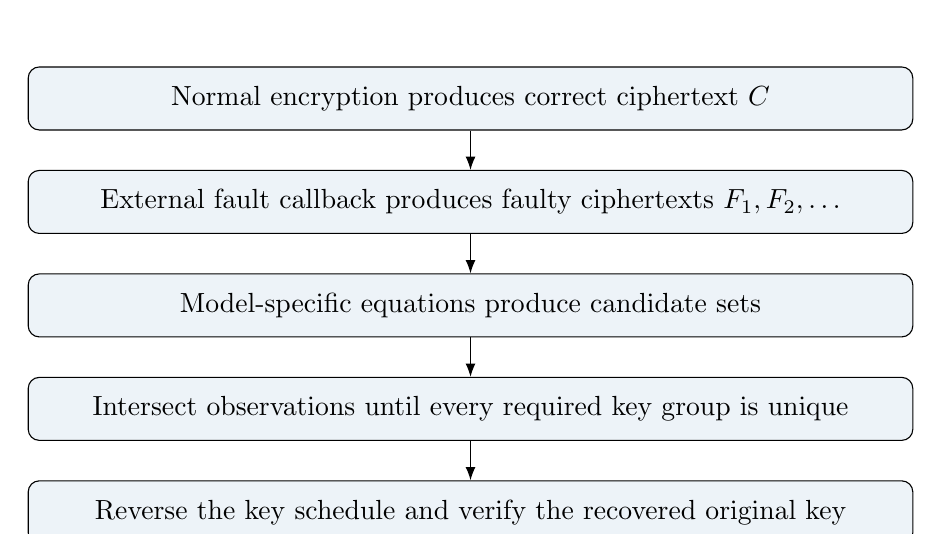
\begin{tikzpicture}[node distance=5mm,box/.style={draw,rounded corners,fill=pale,text width=11cm,align=center,minimum height=8mm},>=Latex]
\node[box] (a) {Normal encryption produces correct ciphertext $C$};
\node[box,below=of a] (b) {External fault callback produces faulty ciphertexts $F_1,F_2,\ldots$};
\node[box,below=of b] (c) {Model-specific equations produce candidate sets};
\node[box,below=of c] (d) {Intersect observations until every required key group is unique};
\node[box,below=of d] (e) {Reverse the key schedule and verify the recovered original key};
\foreach \x/\y in {a/b,b/c,c/d,d/e}{\draw[->] (\x)--(\y);}
\end{tikzpicture}
\end{center}

\section{AES Piret-style attack: code from injection to the master key}
\subsection{Inject into the real AES implementation}
\texttt{encrypt\_\allowbreak{}with\_\allowbreak{}trace} in \texttt{piret.py} installs an observer on \texttt{aes.aes\_\allowbreak{}encrypt}. The callback waits for \texttt{Before MixColumns} in the selected round and performs \texttt{state[row][column] \textasciicircum{}= mask}. It then saves immutable byte snapshots. A zero mask gives a clean trace; nonzero masks represent controlled software faults. The solver does not receive this mask.
\par\smallskip\noindent\textbf{External Piret fault injection into the real AES engine}\par
\begin{lightcode}
def encrypt_with_trace(plaintext, key, row=0, column=0, mask=0, fault_round=8):
    """Run aes.py itself; this external observer injects and records the fault.

    Round 8 spreads to four key groups. Round 9 reaches one key quartet.
    No second AES implementation is used by the attacker.
    """
    if not (0 <= row < 4 and 0 <= column < 4 and 0 <= mask <= 255 and fault_round in (8, 9)):
        raise ValueError("Fault: row/column 0..3, mask 0..255, round 8 or 9.")
    trace = []

    def observer(number, operation, state):
        if number == fault_round and operation == "Before MixColumns":
            state[row][column] ^= mask
            trace.append((number, "Fault point", aes.state_to_bytes(state)))
        if number > 0 and operation.startswith("After "):
            trace.append((number, operation[6:], aes.state_to_bytes(state)))

    ciphertext = aes.aes_encrypt(plaintext, key, observer=observer)
    return ciphertext, trace
\end{lightcode}

\subsection{Convert one output pair into four-byte key candidates}
For column $c$, the output indices are $p_r=4((c-r)\bmod4)+r$, $r=0,1,2,3$. Under a guess $k_r$ for a final-key byte,
\[
d_r(k_r)=S^{-1}(C_{p_r}\xor k_r)\xor S^{-1}(F_{p_r}\xor k_r).
\]
The code first groups the 256 byte guesses by their resulting difference. It then enumerates the \emph{shared} unknown error row $q$ and error value $e$, requiring all four equations $d_r(k_r)=M_{r,q}e$ at once. The Cartesian product combines only compatible byte lists; it does not independently choose arbitrary surviving bytes. This preserves the quartet correlation without enumerating all $2^{32}$ quartets first.
\par\smallskip\noindent\textbf{Piret candidate quartets with one shared row and error}\par
\begin{lightcode}
def key_candidates(correct, faulty, column):
    """Derive four-byte K10 candidates from ciphertexts only.

    For each guessed byte k, undo final AddRoundKey and SubBytes:
      d = InvSbox[C[p] XOR k] XOR InvSbox[Cfault[p] XOR k].
    All four differences must fit ONE matrix column times ONE unknown error.
    """
    if len(correct) != 16 or len(faulty) != 16:
        raise ValueError("Ciphertexts must each contain exactly 16 bytes.")
    # Each table maps a possible input difference d to compatible byte guesses.
    # Four small lookups avoid brute-force enumeration of all 2^32 quartets.
    tables = []
    for position in output_positions(column):
        table = [[] for _ in range(256)]
        for guess in range(256):
            delta = INV_SBOX[correct[position] ^ guess] ^ INV_SBOX[faulty[position] ^ guess]
            table[delta].append(guess)
        tables.append(table)
    found = set()
    for unknown_row in range(4):
        for unknown_error in range(1, 256):
            # A single shared row/error must satisfy ALL four equations.
            # Independent byte filtering alone would lose this constraint.
            choices = [tables[r][gf_multiply(MIX_MATRIX[r][unknown_row], unknown_error)] for r in range(4)]
            found.update(product(*choices))
    return found
\end{lightcode}

\subsection{Round 9 versus the supported round-8 variant}
The GUI's \texttt{pdf\_\allowbreak{}aes\_\allowbreak{}lesson} and the terminal's \texttt{run.aes\_\allowbreak{}demo} use round 9. Each observation affects one output quartet. These functions intersect \texttt{key\_\allowbreak{}candidates} sets separately for all four columns and place the unique tuples back into their original $K_{10}$ byte positions.

The direct \texttt{piret.py} AES command uses round 8. The additional round spreads the original byte disturbance to all four column groups; each final-round group still satisfies a round-9 one-byte-input differential equation with its own effective error. That effective error is not necessarily the original injected mask. \texttt{recover\_\allowbreak{}last\_\allowbreak{}key} therefore processes all four groups from each faulty output. Its explicit requirement that all sixteen ciphertext bytes change belongs to this round-8 path; it must not be imposed on round-9 observations.
\par\smallskip\noindent\textbf{Round-8 AES recovery: intersect all four output groups}\par
\begin{lightcode}
def recover_last_key(correct, faulty_outputs, observer=None):
    """Attacker API: no master key, plaintext, fault mask or internal states.

    The optional observer is for logging only; it cannot modify candidate sets.
    A None result means ambiguity, never an arbitrary candidate selection.
    """
    if len(correct) != 16:
        raise ValueError("Correct ciphertext must contain 16 bytes.")
    groups, used = [None] * 4, 0
    for used, faulty in enumerate(faulty_outputs, 1):
        if len(faulty) != 16 or any(a == b for a, b in zip(correct, faulty)):
            raise ValueError("Expected 16 changed output bytes for the round-8 byte-fault model.")
        for column in range(4):
            fresh = key_candidates(correct, faulty, column)
            before = None if groups[column] is None else len(groups[column])
            # An intersection can retain/remove candidates, never introduce new ones.
            groups[column] = fresh if groups[column] is None else groups[column] & fresh
            if not groups[column]:
                raise ValueError("Empty candidate intersection: incompatible ciphertexts or fault model.")
            if observer:
                observer(used, column, before, len(fresh), tuple(sorted(groups[column])))
        if all(len(group) == 1 for group in groups):
            # Group tuples are in pre-ShiftRows row order. Restore true K10 order.
            last_key = bytearray(16)
            for column in range(4):
                for position, byte in zip(output_positions(column), next(iter(groups[column]))):
                    last_key[position] = byte
            return bytes(last_key), used
    return None, used
\end{lightcode}

\subsection{Recover the original AES key}
Once $K_{10}$ is unique, \texttt{reverse\_\allowbreak{}key\_\allowbreak{}schedule} initializes $w_{40},\ldots,w_{43}$ and walks downward. It computes each earlier word with XOR and the forward key-schedule transformation. It never reads the original key. The forward S-box is correct here because its input schedule word is already known.
\par\smallskip\noindent\textbf{Reverse AES-128 expansion to recover the original key}\par
\begin{lightcode}
def reverse_key_schedule(last_key, observer=None):
    """AES-128 recurrence reversed: w[i-4] = w[i] XOR transform(w[i-1]).

    Descending order guarantees that both right-hand words are already known.
    Reversal still uses the FORWARD S-box: its input word is known, so there
    is no reason to invert SubWord. This function never reads the master key.
    """
    if len(last_key) != 16:
        raise ValueError("K10 must contain 16 bytes.")
    words = [None] * 44
    # K10 occupies the final four schedule words, w40 through w43.
    words[40:] = [list(last_key[index:index+4]) for index in range(0, 16, 4)]
    for index in range(43, 3, -1):
        transformed = words[index - 1][:]
        if index % 4 == 0:
            # Same RotWord/SubWord/Rcon transformation as forward expansion.
            transformed = [SBOX[byte] for byte in transformed[1:] + transformed[:1]]
            transformed[0] ^= aes.RCON[index // 4]
        words[index - 4] = [a ^ b for a, b in zip(words[index], transformed)]
        if observer:
            observer(index, bytes(words[index]), bytes(transformed), bytes(words[index - 4]))
    return bytes(sum(words[:4], []))
\end{lightcode}

If a group still has more than one candidate, the lesson reports ambiguity instead of guessing a key. Increasing the number of observations can help, but no fixed success count is guaranteed for every target state and fault sequence.

\section{AES Giraud attack: one-bit filtering and complete recovery}
\subsection{External fault before final SubBytes}
\texttt{giraud.aes\_\allowbreak{}fault\_\allowbreak{}encrypt} changes one bit in the state immediately before final-round SubBytes. Byte index $b$ maps to \texttt{state[b \% 4][b // 4]}, consistent with AES column-major storage. Unlike the Piret fault, no MixColumns follows this location; one altered S-box input byte reaches one ciphertext byte after ShiftRows.
\par\smallskip\noindent\textbf{External single-bit fault before final AES SubBytes}\par
\begin{lightcode}
def aes_fault_encrypt(plaintext, key, byte=0, mask=None):
    """Interfere with the real aes.py execution before final SubBytes.

    Only this attack callback changes the state. Without it AES is unchanged.
    Snapshots are copies for teaching; they are never inputs to the solver.
    """
    if not 0 <= byte < 16:
        raise ValueError("AES input byte must be 0..15.")
    if mask is not None:
        validate_mask(mask)
    trace = {}

    def observer(number, operation, state):
        if number == 10 and operation == "Before SubBytes":
            trace["Before fault"] = aes.state_to_bytes(state)
            if mask is not None:
                state[byte % 4][byte // 4] ^= mask
            trace["Injected bit"] = aes.state_to_bytes(state)
        if number == 10 and operation.startswith("After "):
            name = "Ciphertext" if operation == "After AddRoundKey" else operation[6:]
            trace[name] = aes.state_to_bytes(state)

    ciphertext = aes.aes_encrypt(plaintext, key, observer=observer)
    return ciphertext, trace
\end{lightcode}

\subsection{Why the filter works}
\texttt{giraud.aes\_\allowbreak{}candidates}, listed in the implementation chapter, first requires exactly one changed output byte. For each $k\in\{0,\ldots,255\}$, it computes
\[
\delta(k)=S^{-1}(C_j\xor k)\xor S^{-1}(F_j\xor k).
\]
In unknown-bit mode, it keeps $k$ when $\delta(k)\in\{1,2,4,8,16,32,64,128\}$. In known-bit mode, it requires the stronger condition $\delta(k)=e$ for the supplied exact mask. A one-bit difference is required at the \emph{inverse-S-box input comparison}, not necessarily in the observed ciphertext XOR.

\texttt{giraud.masks\_\allowbreak{}for} generates up to eight distinct single-bit observations per target byte. \texttt{giraud.intersect\_\allowbreak{}candidates} intersects the resulting sets. The terminal \texttt{main} and GUI \texttt{giraud\_\allowbreak{}lesson} repeat this for all sixteen input byte positions, use the observed output index after ShiftRows to assemble $K_{10}$, and call \texttt{piret.reverse\_\allowbreak{}key\_\allowbreak{}schedule}. Even after all eight masks, an ambiguous byte must remain reported as ambiguous. Knowing the fault location does not imply knowing its exact bit.

\section{SM4 controlled-byte DFA: code and full-key extension}
\subsection{Inject before tau and undo output diffusion}
\texttt{piret.sm4\_\allowbreak{}fault\_\allowbreak{}encrypt} attaches an observer to \texttt{sm4.sm4\_\allowbreak{}encrypt\_\allowbreak{}block}. At \texttt{Sbox input}, it applies \texttt{mask << (24 - 8*byte)} to the 32-bit value. The shift preserves big-endian byte numbering. Its diagnostic trace may contain subkeys for teaching; the oracle passed to the solver returns only the faulty ciphertext.

At target round $i$,
\[
A_i=X_{i+1}\xor X_{i+2}\xor X_{i+3}\xor rk_i,
\qquad X_{i+4}=X_i\xor L(\tau(A_i)).
\]
When the round is last in the current view, only $X_{i+4}$ changes. Since $L$ is XOR-linear,
\[
\Delta B_i=L^{-1}(X_{i+4}\xor X'_{i+4}).
\]
\texttt{inverse\_\allowbreak{}rows} constructs the $32\times32$ binary matrix of $L$ and inverts it by Gaussian elimination. \texttt{inverse\_\allowbreak{}linear} applies the inverse through binary dot products. This is an inverse of the data diffusion map, not the key-schedule map $L'$.
\subsection{Turn S-box input guesses into key-byte guesses}
For the known fault byte $e$, enumerate $a$ satisfying $S(a)\xor S(a\xor e)=\Delta B_{i,b}$. Let $q$ be byte $b$ of $X_{i+1}\xor X_{i+2}\xor X_{i+3}$, available in the other three words of the view. Then a compatible subkey byte is $a\xor q$. The function validates the unchanged words and single-byte support of $\Delta B_i$ before filtering.
\par\smallskip\noindent\textbf{Known-byte SM4 differential filtering}\par
\begin{lightcode}
def sm4_byte_candidates(correct, faulty, byte, mask):
    """Attacker API: outputs and the PDF's KNOWN fault byte/value only."""
    if len(correct) != 16 or len(faulty) != 16 or not 0 <= byte < 4 or not 1 <= mask <= 255:
        raise ValueError("Invalid SM4 output or known-fault descriptor.")
    c, f = struct.unpack(">4I", correct), struct.unpack(">4I", faulty)
    if c[1:] != f[1:]:
        raise ValueError("The last-round model requires three output words unchanged.")
    delta_b = inverse_linear(c[0] ^ f[0])
    shift = 24 - 8 * byte
    if not delta_b or delta_b & ~(255 << shift):
        raise ValueError("Difference does not match a single-byte S-box input fault.")
    d = (delta_b >> shift) & 255
    known = ((c[1] ^ c[2] ^ c[3]) >> shift) & 255
    inputs = {a for a in range(256) if sm4.SBOX[a] ^ sm4.SBOX[a ^ mask] == d}
    return {a ^ known for a in inputs}, inputs, delta_b
\end{lightcode}

\subsection{Recover four subkeys instead of supplying three reference values}
A single last-round experiment recovers at most $rk_{31}$, which is only 32 bits. The implemented \texttt{piret.recover\_\allowbreak{}sm4\_\allowbreak{}master\_\allowbreak{}key} extends the model:
\begin{enumerate}
\item Recover all four bytes of $rk_{31}$ using faults in round 31.
\item Request new faulty outputs from round 30. Undo round 31 on \emph{both} correct and faulty outputs using the recovered $rk_{31}$.
\item Apply the same last-round equations to this restored round-30 view to recover $rk_{30}$.
\item Repeat at round 29, then round 28, undoing only later rounds whose keys have already been recovered.
\item Pass the recovered keys in the order $[rk_{28},rk_{29},rk_{30},rk_{31}]$ to \texttt{reverse\_\allowbreak{}sm4}.
\end{enumerate}
For a rolling window $(X_{i+1},X_{i+2},X_{i+3},X_{i+4})$ and a known recovered $rk_i$, the previous word is
\[
X_i=X_{i+4}\xor L\bigl(\tau(X_{i+1}\xor X_{i+2}\xor X_{i+3}\xor rk_i)\bigr).
\]
This is the equation implemented by \texttt{peel\_\allowbreak{}sm4}, already listed in the implementation chapter. The returned view uses reversed word order so that \texttt{sm4\_\allowbreak{}byte\_\allowbreak{}candidates} can reuse its output equations. An earlier-round fault may affect several words of the \emph{raw} final ciphertext; the three-unchanged-word condition is checked after the appropriate peeling.

The full recovery function's inputs are a correct output, a callable \texttt{fault\_\allowbreak{}oracle(round, byte, mask)}, and model configuration. It receives neither plaintext nor a key schedule. The oracle closure knows the simulation key only to run the target. If any byte remains ambiguous, the function returns \texttt{complete=False} and \texttt{master\_\allowbreak{}key=None}; it never peels an unrecovered round with a reference key.

\texttt{reverse\_\allowbreak{}sm4} reverses $K_{i+4}=K_i\xor T'(K_{i+1}\xor K_{i+2}\xor K_{i+3}\xor CK_i)$, using $T'=L'\circ\tau$. After obtaining $K_0,\ldots,K_3$, it XORs the fixed $FK_i$ constants to recover the four original master-key words. Four consecutive round keys are required; knowledge of $rk_{31}$ alone is insufficient.

\section{SM4 Giraud-inspired attack: reuse with a different filter}
\texttt{giraud.sm4\_\allowbreak{}fault\_\allowbreak{}encrypt} validates that the simulator mask is a single bit, then reuses the actual SM4 target adapter. \texttt{giraud.sm4\_\allowbreak{}candidates}, listed earlier, computes $L^{-1}(\Delta X)$ and identifies the changed S-box byte. For each candidate input $a$, unknown-bit mode accepts it if
\[
\exists e\in\{1,2,4,8,16,32,64,128\}:\quad S(a)\xor S(a\xor e)=\Delta B_b.
\]
Known-bit mode tests only the specified $e$. The surviving $a$ values are converted to subkey candidates with the same observable-word XOR as the controlled-byte model.

The following wrapper changes only the candidate filter. It keeps the sequential round recovery, intersections, peeling, and key-schedule reversal shared with the byte-DFA engine. In particular, the parameter \texttt{simulator\_\allowbreak{}mask} is deliberately not forwarded to \texttt{sm4\_\allowbreak{}candidates} in unknown-bit mode.
\par\smallskip\noindent\textbf{Giraud-inspired SM4 wrapper with explicit mask knowledge}\par
\begin{lightcode}
def recover_sm4_master_key(correct, fault_oracle, first_mask=1, maximum=8, known_bit=False, start_byte=0, observer=None):
    """Full SM4 recovery using single-bit filtering in rounds 31, 30, 29, 28."""
    import piret

    def candidate_filter(clean, faulty, simulator_mask):
        # Unknown-bit mode deliberately does not pass the oracle's mask onward.
        return sm4_candidates(clean, faulty, simulator_mask if known_bit else None)

    return piret.recover_sm4_master_key(correct, fault_oracle, masks_for(first_mask, maximum), start_byte, candidate_filter, observer)
\end{lightcode}

This division explains why two attacks share a full-key recovery engine without being identical: the allowed error sets and the information supplied to the filter differ. Both require controlled faults at each of rounds 31--28 for full recovery in this implementation.

\section{How the GUI maps to the attack code}
Run \texttt{python src/gui.py} from the repository root. Select the algorithm and operation, load a standard example or enter a 16-byte hexadecimal key and block, then build the lesson.
\begin{itemize}
\item \textbf{Encrypt / Decrypt:} \texttt{aes\_\allowbreak{}trace} or \texttt{sm4\_\allowbreak{}trace} observes normal transformations. The inverse operation verifies the input block is recovered.
\item \textbf{AES / Fault analysis:} \texttt{pdf\_\allowbreak{}aes\_\allowbreak{}lesson} uses the round-9 Piret path, processes all four columns and recovers $K_0$.
\item \textbf{SM4 / Fault analysis:} \texttt{pdf\_\allowbreak{}sm4\_\allowbreak{}lesson} calls \texttt{sm4\_\allowbreak{}master\_\allowbreak{}lesson} with the known-byte filter.
\item \textbf{Giraud attack:} \texttt{giraud\_\allowbreak{}lesson} uses the AES byte filter or routes SM4 to \texttt{sm4\_\allowbreak{}master\_\allowbreak{}lesson} with the single-bit filter. The exact-bit checkbox selects whether the solver receives the mask.
\end{itemize}
The GUI row/byte and column fields choose the initial demonstration coordinate, not a restriction to recovering only one key byte. The maximum-observation setting is per target group or byte. A lesson snapshot stores the round, operation, explanation, 16-byte displayed state, details and optional correct reference. Normal steps compare with the previous displayed state; fault steps compare with the corresponding correct state. Red nonzero XOR bytes visualize these comparisons. SM4 scalar intermediates $A$, $\tau(A)$ and $L(\tau(A))$ appear in the details; the rolling state does not change until the new word is appended.

\section{Commands and verified default examples}
\begin{lightcode}
# GUI: both algorithms and both fault-analysis models
python src/gui.py
# AES round-8 Piret-style terminal lesson
python src/piret.py --algorithm aes
# AES round-9 Piret and controlled-byte SM4 DFA
python src/run.py
# Controlled-byte SM4 full master-key recovery
python src/piret.py --algorithm sm4
# Unknown-bit Giraud models (default)
python src/giraud.py --algorithm aes
python src/giraud.py --algorithm sm4
# Stronger model: exact single-bit mask given to the solver
python src/giraud.py --algorithm aes --known-bit
python src/giraud.py --algorithm sm4 --known-bit
\end{lightcode}
On 7 November 2026, the following GUI lesson builders were executed directly without opening a window. Coordinates were zero, first mask was \hex{01}, maximum observations was eight, and Giraud used its default unknown-bit mode. The official inputs and keys given earlier were used.
\begin{center}
\small
\begin{tabular}{P{.34\linewidth}rl}
\toprule Lesson & Faulty outputs used & Recovered original key\\\midrule
AES round-9 Piret & 8 & \hex{00010203\allowbreak{}04050607\allowbreak{}08090A0B\allowbreak{}0C0D0E0F}\\
AES Giraud, unknown bit & 35 & \hex{00010203\allowbreak{}04050607\allowbreak{}08090A0B\allowbreak{}0C0D0E0F}\\
SM4 known-byte DFA & 32 & \hex{01234567\allowbreak{}89ABCDEF\allowbreak{}FEDCBA98\allowbreak{}76543210}\\
SM4 Giraud-inspired, unknown bit & 35 & \hex{01234567\allowbreak{}89ABCDEF\allowbreak{}FEDCBA98\allowbreak{}76543210}\\
\bottomrule
\end{tabular}
\end{center}
All four returned \texttt{verified=True}. These counts describe these particular deterministic examples, not a bound for arbitrary keys, plaintexts, masks or physical targets. Earlier terminal excerpts use the explicitly known-bit model, which explains why their counts can differ.

\section{Validation and limits of the implementation}
The regression suite checks known-answer vectors, inverse operations, fault propagation, candidate intersections, key-schedule reversal and ambiguous cases. \texttt{tests/test\_\allowbreak{}cipher\_\allowbreak{}separation.py} checks that the attacks intervene in the real cipher engines. \texttt{tests/test\_\allowbreak{}sm4\_\allowbreak{}full\_\allowbreak{}recovery.py} tests random keys with a precomputed output-only oracle and blocks \texttt{sm4.key\_\allowbreak{}expansion} while the recovery solver executes. This guards against accidentally obtaining the key from a reference schedule. \texttt{tests/test\_\allowbreak{}giraud.py} checks known/unknown-bit filtering and recovery for both algorithms.
\begin{lightcode}
python -m unittest discover -s tests -v
python tests/test_crypto_lab.py --gui CryptoTests.test_gui
\end{lightcode}
The simulated observer is more precise than an uncharacterized physical glitch: it selects a round, intermediate value and bit/byte. No runtime trace or known test key is evidence that a ChipWhisperer glitch on STM32F303 satisfies that model. Physical evaluation must establish the observed fault support and location, then report useful-fault rate, ambiguity and key recovery separately. No additional hardware results are claimed by this code walkthrough.


\fi

\SelectPart{3}
\ifshowpart
  \chapter{Implementation Manual: Every Function and Its Execution Order}
\label{chap:function-manual}
This manual explains every named function, class method and nested callback in the six executable source modules. It complements the mathematical chapters with the actual implementation order, arguments, state changes, return values and interactions. Constants, module initialization, lambdas and main guards are explained separately. The appendix contains the complete source snapshot, including imports, tables, comments and entry points, so this document can be read without opening an external Python file.

\section{Reading Python data and control flow}
\begin{itemize}
\item A byte is an integer from zero to 255; immutable \texttt{bytes} are used for external blocks and stored snapshots. \texttt{list} and nested row lists hold mutable working states. Reassigning an element of an AES matrix changes that matrix; replacing a local integer requires returning the replacement.
\item \texttt{\^{}} is XOR, \texttt{\&} is bitwise AND, and shifts move bits. \texttt{0xFF} keeps eight low bits and \texttt{0xFFFFFFFF} keeps thirty-two. These operators are not ordinary addition and multiplication.
\item \texttt{[a:b]} copies a slice; \texttt{[::-1]} reverses order. AES row rotation moves bytes inside one row; SM4's final reversal moves four entire words. These operations must not be confused.
\item \texttt{None} means no value/observer or no observation yet. A nonempty candidate set with multiple elements means ambiguity. Empty intersections are model errors, not successful recovery of zero-valued key bytes.
\item An observer is a function passed to another function. A closure captures values from its containing execution. A generator yields observations only when the solver asks for them. These constructs connect the existing engines to the experiments without copying the encryption algorithms.
\item Each \texttt{if \_\allowbreak{}\_\allowbreak{}name\_\allowbreak{}\_\allowbreak{} == "\_\allowbreak{}\_\allowbreak{}main\_\allowbreak{}\_\allowbreak{}"} block runs only on direct execution. Importing a module defines its helpers and constants without automatically starting its terminal demonstration or opening a Tk window.
\end{itemize}

\section{Module-level configuration and initialization}
\begin{description}
\item[\texttt{aes.py}] \texttt{KEY} and \texttt{PLAINTEXT} are editable demonstration strings, not implicit inputs to the block functions. \texttt{BLOCK\_\allowbreak{}SIZE=16} and \texttt{N\_\allowbreak{}ROUNDS=10} select AES-128. \texttt{SBOX} contains the standard substitution table; \texttt{INV\_\allowbreak{}SBOX} is constructed by reversing its mapping. \texttt{RCON} uses an unused index zero so schedule rounds index directly. \texttt{MIX\_\allowbreak{}MATRIX} and \texttt{INV\_\allowbreak{}MIX\_\allowbreak{}MATRIX} contain the field coefficients for forward/inverse column mixing.
\item[\texttt{sm4.py}] The example strings use the official vector. \texttt{WORD\_\allowbreak{}MASK} bounds words to thirty-two bits; \texttt{BLOCK\_\allowbreak{}SIZE} and \texttt{N\_\allowbreak{}ROUNDS} select sixteen bytes and thirty-two rounds. The SM4 \texttt{SBOX} is different from AES. Four \texttt{FK} words initialize the key schedule; thirty-two \texttt{CK} words enter the schedule recurrence. Their byte construction is documented next to the constants in the source.
\item[\texttt{piret.py}] Imports expose the real cipher engines, Cartesian products for correlated quartet candidates, a cached inverse binary matrix, random fault sequences and terminal formatting. The legacy key/plaintext/fault globals are for \texttt{relation\_\allowbreak{}demo}; the main recovery path reads the cipher configuration or explicit parameters. The inverse AES S-box and mixing matrix are shared mathematical data, not a secret key.
\item[\texttt{giraud.py}] \texttt{SINGLE\_\allowbreak{}BITS} enumerates the eight possible one-bit byte masks. \texttt{AES\_\allowbreak{}INVERSE\_\allowbreak{}SBOX} is public algorithm data. The inverse SM4 data diffusion function is imported from the common attack module. Mask knowledge is an explicit argument, not inferred from the simulator's hidden state.
\item[\texttt{run.py}] Imports the target engines and common attack mathematics. \texttt{LessonTerminal} extends \texttt{piret.Terminal} with flat byte comparisons; its inherited color and pause behavior remains presentation only.
\item[\texttt{gui.py}] Imports JSON export, queue/thread support and Tk widgets, then the cipher/attack modules. \texttt{AES\_\allowbreak{}KEY}, \texttt{AES\_\allowbreak{}INPUT} and \texttt{SM4\_\allowbreak{}VECTOR} define examples. Color constants style the window. Its extra inverse-S-box table is module-level teaching data; candidate solving still delegates to the attack modules. The main guard creates the Tk root, constructs \texttt{CryptoLab} and enters \texttt{mainloop}.
\end{description}

\section{End-to-end trace: ordinary AES and SM4}
\begin{enumerate}
\item In AES, \texttt{aes\_\allowbreak{}encrypt(P,K)} first calls \texttt{bytes\_\allowbreak{}to\_\allowbreak{}state(P)} and \texttt{key\_\allowbreak{}expansion(K)}. The initial state byte at row one, column zero is \hex{11}; its matching first-key byte is \hex{01}, so the initial XOR produces \hex{10}.
\item \texttt{\_\allowbreak{}operation} applies the initial key and each subsequent transformation. At round one, \texttt{sub\_\allowbreak{}bytes} replaces \hex{10} by \hex{CA}; \texttt{shift\_\allowbreak{}rows} moves it to another column; \texttt{mix\_\allowbreak{}columns} combines column bytes using \texttt{gf\_\allowbreak{}mul}. \texttt{add\_\allowbreak{}round\_\allowbreak{}key} then applies K1.
\item The AES loop repeats until round ten, whose conditional skips MixColumns. \texttt{state\_\allowbreak{}to\_\allowbreak{}bytes} returns \hex{69C4E0D8\allowbreak{}6A7B0430\allowbreak{}D8CDB780\allowbreak{}70B4C55A} for the official vector. Decryption starts with K10 and reverses the transformations to recover P.
\item In SM4, \texttt{sm4\_\allowbreak{}encrypt\_\allowbreak{}block(P,K)} delegates to \texttt{sm4\_\allowbreak{}process\_\allowbreak{}block}. It unpacks P into X0 through X3 and calls \texttt{key\_\allowbreak{}expansion}. The first encryption subkey is \hex{F12186F9}.
\item \texttt{round} forms A0=\hex{F002C39E}, applies \texttt{sbox} to obtain \hex{18E992B1}, and \texttt{linear} to obtain \hex{26D99622}. XOR with X0=\hex{01234567} gives X4=\hex{27FAD345}. The returned window is X1,X2,X3,X4.
\item After thirty-two updates, SM4 serializes X35,X34,X33,X32, producing \hex{681EDF34\allowbreak{}D206965E\allowbreak{}86B3E94F\allowbreak{}536E4246}. The decryption wrapper uses the same recurrence with the subkeys in reverse order and checks the original block is recovered.
\end{enumerate}

\section{End-to-end trace: the four fault-recovery paths}
\begin{enumerate}
\item \textbf{AES round-nine Piret:} \texttt{pdf\_\allowbreak{}aes\_\allowbreak{}lesson} or \texttt{run.aes\_\allowbreak{}demo} asks \texttt{encrypt\_\allowbreak{}with\_\allowbreak{}trace} for a byte fault. Its observer mutates the real AES state before MixColumns. \texttt{key\_\allowbreak{}candidates} receives only the output pair and column; intersections recover a quartet. After four unique groups, \texttt{reverse\_\allowbreak{}key\_\allowbreak{}schedule} reconstructs K0. The direct \texttt{piret.py} command instead uses the documented round-eight generator and \texttt{recover\_\allowbreak{}last\_\allowbreak{}key} to process all groups together.
\item \textbf{AES Giraud:} \texttt{aes\_\allowbreak{}fault\_\allowbreak{}encrypt} changes one bit before final SubBytes. \texttt{aes\_\allowbreak{}candidates} identifies the single changed output byte and tests the inverse-S-box equation for every byte guess. \texttt{intersect\_\allowbreak{}candidates} retains shared survivors. Each unique output byte fills its K10 position; reversal and re-encryption follow only after all sixteen positions are unique.
\item \textbf{SM4 byte DFA:} \texttt{recover\_\allowbreak{}sm4\_\allowbreak{}master\_\allowbreak{}key} asks an output-only oracle for a selected round/byte/mask. \texttt{peel\_\allowbreak{}sm4} removes already recovered later rounds, and \texttt{sm4\_\allowbreak{}byte\_\allowbreak{}candidates} removes L from the difference. Intersections identify a subkey byte. All sixteen subkey bytes across rounds 31--28 must be unique before \texttt{reverse\_\allowbreak{}sm4} returns the master key.
\item \textbf{SM4 Giraud-inspired:} the same outer recovery loop runs, but the wrapper supplies \texttt{sm4\_\allowbreak{}candidates} through \texttt{candidate\_\allowbreak{}filter}. Unknown-bit mode tests all eight bit masks and never forwards the actual simulator mask. Controlled target access at all four rounds is still required; changing the filter does not remove that assumption.
\end{enumerate}
These paths share data structures and target engines, but their observation requirements and allowed fault sets differ. A teaching observer is allowed to show an intermediate value; the recovery API is not automatically entitled to receive it.

\section{How to use the function reference}
Every entry below gives the actual callable signature, its source line range in the appendix, and ordered implementation steps. Methods include \texttt{self}, the application or terminal instance on which they operate. Nested callbacks are described after their containing module. The appendix retains decorators, including the cached inverse-matrix decorator, as well as complete parent functions containing the callbacks. Signature wrapping in the typeset listing does not change the one-line argument convention in the source files. Code uses plain monospaced rendering to reduce compilation work; all source text is retained. The contents lists chapters and sections, while individual function headings remain in the body.

\section{\texttt{aes.py}: function-by-function implementation}
Read conversion first, then field arithmetic, transformations, key expansion, encryption and inverse operations. Matrix transformations mutate their argument and return None; block functions return immutable bytes. The operation wrapper is the only generic instrumentation seam.
\subsection{\texttt{validate\_\allowbreak{}block}}
\begin{lightcode}
def validate_block(data, label="Block"):
\end{lightcode}
\noindent\textbf{Source:} complete \texttt{aes.py} listing in Part 6, lines 101--104.
\begin{enumerate}
\item Accept a byte sequence and a human-readable label. Check its length against BLOCK\_SIZE, which is sixteen.
\item Raise ValueError on a wrong length; otherwise return None. This validates size, not message padding or a general encryption mode.
\end{enumerate}
\subsection{\texttt{bytes\_\allowbreak{}to\_\allowbreak{}state}}
\begin{lightcode}
def bytes_to_state(data):
\end{lightcode}
\noindent\textbf{Source:} complete \texttt{aes.py} listing in Part 6, lines 107--116.
\begin{enumerate}
\item Validate the sixteen input elements and allocate four independent rows.
\item Traverse columns outside rows and assign data[4*column+row] to state[row][column]. Return a fresh mutable matrix, so later transformations do not mutate the caller's bytes.
\end{enumerate}
\subsection{\texttt{state\_\allowbreak{}to\_\allowbreak{}bytes}}
\begin{lightcode}
def state_to_bytes(state):
\end{lightcode}
\noindent\textbf{Source:} complete \texttt{aes.py} listing in Part 6, lines 119--121.
\begin{enumerate}
\item Traverse the matrix column by column in exactly the inverse conversion order.
\item Construct and return immutable bytes. For example, matrix entry state[1][2] becomes output byte nine, not byte six.
\end{enumerate}
\subsection{\texttt{xtime}}
\begin{lightcode}
def xtime(a):
\end{lightcode}
\noindent\textbf{Source:} complete \texttt{aes.py} listing in Part 6, lines 129--137.
\begin{enumerate}
\item Shift the byte left once to multiply its polynomial by x. Test the original high bit to detect the x\textasciicircum{}8 overflow.
\item If that bit was set, XOR 0x1B into the shifted result, then mask to eight bits. Thus xtime(0x80) is 0x1B, not the ordinary integer product 0x100.
\end{enumerate}
\subsection{\texttt{gf\_\allowbreak{}mul}}
\begin{lightcode}
def gf_mul(a, b):
\end{lightcode}
\noindent\textbf{Source:} complete \texttt{aes.py} listing in Part 6, lines 140--152.
\begin{enumerate}
\item Initialize an XOR accumulator and inspect eight bits of multiplier b. Whenever the low bit is one, XOR the current multiplicand a into the result.
\item Advance a with xtime and shift b right after each iteration. Return one field byte; multiplication by 02 and 03 in MixColumns therefore uses field reduction rather than ordinary multiplication.
\end{enumerate}
\subsection{\texttt{sub\_\allowbreak{}bytes}}
\begin{lightcode}
def sub_bytes(state):
\end{lightcode}
\noindent\textbf{Source:} complete \texttt{aes.py} listing in Part 6, lines 160--168.
\begin{enumerate}
\item Visit every state coordinate and use its current byte as an index into SBOX.
\item Overwrite that coordinate with the substituted byte. Return None: this operation changes values in the supplied matrix in place, without changing their positions.
\end{enumerate}
\subsection{\texttt{shift\_\allowbreak{}rows}}
\begin{lightcode}
def shift_rows(state):
\end{lightcode}
\noindent\textbf{Source:} complete \texttt{aes.py} listing in Part 6, lines 171--174.
\begin{enumerate}
\item For row indices one through three, split the row after its row index.
\item Concatenate the suffix and prefix to rotate that row left by its index. Row zero stays fixed, and the function updates the matrix in place without returning a new state.
\end{enumerate}
\subsection{\texttt{mix\_\allowbreak{}column}}
\begin{lightcode}
def mix_column(column):
\end{lightcode}
\noindent\textbf{Source:} complete \texttt{aes.py} listing in Part 6, lines 177--189.
\begin{enumerate}
\item Accept four original column bytes and initialize an empty output list. For each row of MIX\_MATRIX, XOR the four coefficient/byte products computed by gf\_mul.
\item Append each resulting byte and return the new four-byte list. Keeping the original column separate prevents an earlier output assignment from contaminating a later equation.
\end{enumerate}
\subsection{\texttt{mix\_\allowbreak{}columns}}
\begin{lightcode}
def mix_columns(state):
\end{lightcode}
\noindent\textbf{Source:} complete \texttt{aes.py} listing in Part 6, lines 192--197.
\begin{enumerate}
\item Extract one column into an independent four-element list and call mix\_column.
\item Write its four returned bytes back to the same column and repeat for all four columns. The state is updated in place; no printing or fault rule is introduced.
\end{enumerate}
\subsection{\texttt{add\_\allowbreak{}round\_\allowbreak{}key}}
\begin{lightcode}
def add_round_key(state, round_key):
\end{lightcode}
\noindent\textbf{Source:} complete \texttt{aes.py} listing in Part 6, lines 200--208.
\begin{enumerate}
\item Read the state and round-key matrices at matching row/column coordinates.
\item XOR each key byte into the state byte in place. Applying the same key twice undoes the operation, and applying it to both members of a differential pair preserves their XOR difference.
\end{enumerate}
\subsection{\texttt{rot\_\allowbreak{}word}}
\begin{lightcode}
def rot_word(word):
\end{lightcode}
\noindent\textbf{Source:} complete \texttt{aes.py} listing in Part 6, lines 216--218.
\begin{enumerate}
\item Take a four-byte key-schedule word and slice off its first byte.
\item Append that byte after the other three and return a new list. This rotates key-word bytes, not bits, and leaves the argument unchanged.
\end{enumerate}
\subsection{\texttt{sub\_\allowbreak{}word}}
\begin{lightcode}
def sub_word(word):
\end{lightcode}
\noindent\textbf{Source:} complete \texttt{aes.py} listing in Part 6, lines 221--223.
\begin{enumerate}
\item Take each byte of a key-schedule word as an SBOX index.
\item Return a new four-byte list of substituted values. This uses the same forward AES S-box as encryption, not INV\_SBOX.
\end{enumerate}
\subsection{\texttt{key\_\allowbreak{}expansion}}
\begin{lightcode}
def key_expansion(key):
\end{lightcode}
\noindent\textbf{Source:} complete \texttt{aes.py} listing in Part 6, lines 226--259.
\begin{enumerate}
\item Validate the master key and divide it into four four-byte words. Generate words four through forty-three by XORing the word four places back with a transformed copy of the previous word.
\item On every fourth word, first apply rot\_word, sub\_word and RCON to the first byte. Group each four consecutive words into a fresh state matrix and return eleven matrices K0 through K10.
\end{enumerate}
\subsection{\texttt{\_\allowbreak{}operation}}
\begin{lightcode}
def _operation(state, number, name, transform, observer):
\end{lightcode}
\noindent\textbf{Source:} complete \texttt{aes.py} listing in Part 6, lines 267--277.
\begin{enumerate}
\item Accept a mutable state, round number, operation name, transformation callable and optional observer. If present, notify the observer with a Before event and the live state.
\item Run transform(state), then issue the corresponding After event. The observer can modify the live matrix; the cipher itself defines no coordinate or XOR mask for an attack.
\end{enumerate}
\subsection{\texttt{aes\_\allowbreak{}encrypt}}
\begin{lightcode}
def aes_encrypt(plaintext, key, observer=None):
\end{lightcode}
\noindent\textbf{Source:} complete \texttt{aes.py} listing in Part 6, lines 280--291.
\begin{enumerate}
\item Convert the plaintext to a matrix, expand the key and apply the initial AddRoundKey with K0 through \_operation.
\item Run rounds one through ten in SubBytes, ShiftRows, optional MixColumns, AddRoundKey order. Skip MixColumns in round ten, serialize the final matrix and return ciphertext bytes without printing.
\end{enumerate}
\subsection{\texttt{inv\_\allowbreak{}sub\_\allowbreak{}bytes}}
\begin{lightcode}
def inv_sub_bytes(state):
\end{lightcode}
\noindent\textbf{Source:} complete \texttt{aes.py} listing in Part 6, lines 294--298.
\begin{enumerate}
\item Read each current state byte and index INV\_SBOX.
\item Replace the byte in place. The inverse table undoes the forward substitution independently at each coordinate.
\end{enumerate}
\subsection{\texttt{inv\_\allowbreak{}shift\_\allowbreak{}rows}}
\begin{lightcode}
def inv_shift_rows(state):
\end{lightcode}
\noindent\textbf{Source:} complete \texttt{aes.py} listing in Part 6, lines 301--304.
\begin{enumerate}
\item Visit rows one through three and split each row before its final row-index bytes.
\item Move those final bytes to the front. These right rotations undo shift\_rows while leaving row zero unchanged.
\end{enumerate}
\subsection{\texttt{inv\_\allowbreak{}mix\_\allowbreak{}columns}}
\begin{lightcode}
def inv_mix_columns(state):
\end{lightcode}
\noindent\textbf{Source:} complete \texttt{aes.py} listing in Part 6, lines 307--315.
\begin{enumerate}
\item Copy all four original bytes of each column before any assignment.
\item For every output row, XOR products with the corresponding INV\_MIX\_MATRIX coefficients, using gf\_mul, and store the result. The copy ensures every inverse output uses the same original column.
\end{enumerate}
\subsection{\texttt{aes\_\allowbreak{}decrypt}}
\begin{lightcode}
def aes_decrypt(ciphertext, key, observer=None):
\end{lightcode}
\noindent\textbf{Source:} complete \texttt{aes.py} listing in Part 6, lines 318--329.
\begin{enumerate}
\item Convert ciphertext to a state, expand the supplied key and remove K10 with AddRoundKey.
\item Iterate key indices nine down to zero, applying InvShiftRows, InvSubBytes and AddRoundKey, followed by InvMixColumns except at index zero. Serialize and return the recovered plaintext; this is ordinary decryption, not a key-recovery attack.
\end{enumerate}
\subsection{\texttt{main}}
\begin{lightcode}
def main():
\end{lightcode}
\noindent\textbf{Source:} complete \texttt{aes.py} listing in Part 6, lines 332--344.
\begin{enumerate}
\item Decode configured KEY and PLAINTEXT hexadecimal strings, encrypt once and decrypt the result.
\item Print the key, plaintext, ciphertext and recovered block; raise RuntimeError if the recovered input differs. The main guard calls this routine only when aes.py is executed directly.
\end{enumerate}

\subsection{Why the AddRoundKey lambdas are needed}
\texttt{\_\allowbreak{}operation} expects a transformation taking only the current state. An expression such as \texttt{lambda s: add\_\allowbreak{}round\_\allowbreak{}key(s, keys[number])} adapts the two-argument key-XOR primitive to that interface. It is invoked immediately during the current loop iteration; it is not stored for later execution. Consequently it uses the intended round key rather than a later loop index.

\section{\texttt{sm4.py}: function-by-function implementation}
Read word rotations and the two distinct linear maps, then tau, observation semantics, round recurrence, key recurrence and common block processing. Unlike AES, each round returns a replacement four-word window. Encryption and decryption differ in subkey order.

\subsection{Implementation topics and presentation order}
\begin{enumerate}
\item \textbf{Inputs, words and constants.} Introduce the sixteen-byte block/key, four big-endian words, thirty-two rounds, SM4 \texttt{SBOX}, \texttt{FK}, \texttt{CK} and word mask. The SM4 S-box is not the AES S-box.
\item \textbf{Circular rotation.} Explain \texttt{rotl}, its shift/mask operations and how wrapped bits re-enter the word. Follow one 32-bit input through a rotation before introducing the diffusion formulas.
\item \textbf{Substitution and diffusion.} Explain \texttt{sbox} as four independent byte substitutions. Compare \texttt{linear}, using rotations 2, 10, 18 and 24, with \texttt{linear\_key}, using rotations 13 and 23. These maps serve different recurrences.
\item \textbf{Key schedule.} Follow \texttt{generate\_round\_key} and \texttt{key\_expansion}: XOR the master words with FK, slide a four-word window, incorporate CK and generate $rk_0$ through $rk_{31}$.
\item \textbf{One data round.} Trace \texttt{round}: compute $A=X_{i+1}\xor X_{i+2}\xor X_{i+3}\xor rk_i$, then $B=\tau(A)$, $D=L(B)$ and $X_{i+4}=X_i\xor D$. Return the updated four-word window.
\item \textbf{Observation mechanism.} Explain \texttt{observe}: an absent callback preserves the value, None preserves it too, and another returned value replaces it. This is how an external experiment can intervene without embedding an attack model in normal SM4.
\item \textbf{Complete encryption and decryption.} Follow \texttt{sm4\_process\_block}, \texttt{sm4\_encrypt\_block} and \texttt{sm4\_decrypt\_block}. Explain thirty-two updates, final word reversal and reverse subkey order for decryption. Word reversal does not reverse the bytes inside each word.
\item \textbf{Verification and demonstration.} Use \texttt{main} and the official ciphertext to validate the result, then check recovery of the input. Explain that this is a raw-block implementation; message padding and authenticated modes are outside these functions. Terminal logging is handled by the shared wrapper.
\end{enumerate}
\noindent\textbf{Suggested explanation sequence:} block $\rightarrow$ four words $\rightarrow$ key expansion $\rightarrow$ XOR $\rightarrow$ substitution $\rightarrow$ diffusion $\rightarrow$ rolling update $\rightarrow$ final reversal.

\subsection{\texttt{rotl}}
\begin{lightcode}
def rotl(val: int, count: int) -> int:
\end{lightcode}
\noindent\textbf{Source:} complete \texttt{sm4.py} listing in Part 7, lines 71--73.
\begin{enumerate}
\item Accept a 32-bit word and a rotation count used by the fixed SM4 transforms. Shift left, mask the overflowing high bits and shift the original word right by 32-count.
\item OR the two pieces to return a circular left rotation. The fixed call sites use counts two, ten, eighteen, twenty-four, thirteen and twenty-three.
\end{enumerate}
\subsection{\texttt{linear}}
\begin{lightcode}
def linear(b: int) -> int:
\end{lightcode}
\noindent\textbf{Source:} complete \texttt{sm4.py} listing in Part 7, lines 76--82.
\begin{enumerate}
\item Take the 32-bit substituted data word B. Compute rotations by two, ten, eighteen and twenty-four using rotl.
\item XOR B with all four rotations and return L(B). This map is XOR-linear, which permits differential inversion in the SM4 attacks.
\end{enumerate}
\subsection{\texttt{linear\_\allowbreak{}key}}
\begin{lightcode}
def linear_key(b: int) -> int:
\end{lightcode}
\noindent\textbf{Source:} complete \texttt{sm4.py} listing in Part 7, lines 85--87.
\begin{enumerate}
\item Take a word from the key-schedule substitution.
\item XOR it with rotations thirteen and twenty-three and return L-prime. The key schedule deliberately uses a different diffusion map from the data rounds.
\end{enumerate}
\subsection{\texttt{sbox}}
\begin{lightcode}
def sbox(a: int) -> int:
\end{lightcode}
\noindent\textbf{Source:} complete \texttt{sm4.py} listing in Part 7, lines 90--94.
\begin{enumerate}
\item Pack the input word into four big-endian bytes using struct.pack.
\item Substitute each byte through the SM4 SBOX and unpack the four bytes back into a 32-bit word. This implements tau without changing byte order.
\end{enumerate}
\subsection{\texttt{observe}}
\begin{lightcode}
def observe(observer, number, operation, value):
\end{lightcode}
\noindent\textbf{Source:} complete \texttt{sm4.py} listing in Part 7, lines 102--111.
\begin{enumerate}
\item If no observer exists, immediately return the original intermediate value. Otherwise call observer(number, operation, value).
\item Retain the original value when the callback returns None, or return the replacement otherwise. Unlike AES matrix mutation, SM4 callbacks replace immutable integer, tuple or bytes values through this return channel.
\end{enumerate}
\subsection{\texttt{round}}
\begin{lightcode}
def round(x: list[int], rk: int, observer=None, round_index=0):
\end{lightcode}
\noindent\textbf{Source:} complete \texttt{sm4.py} listing in Part 7, lines 114--124.
\begin{enumerate}
\item Accept four rolling state words and the round subkey. Form the XOR of the three newest words and the subkey, then pass it through the Sbox input observation event.
\item Apply sbox and linear with their observation events, XOR the result with the oldest word, and return the three newer words followed by this new word. The input list is not modified in place.
\end{enumerate}
\subsection{\texttt{generate\_\allowbreak{}round\_\allowbreak{}key}}
\begin{lightcode}
def generate_round_key(k: list[int], round: int) -> int:
\end{lightcode}
\noindent\textbf{Source:} complete \texttt{sm4.py} listing in Part 7, lines 127--133.
\begin{enumerate}
\item Accept four consecutive schedule words and a zero-based round index. XOR the three newest words with CK at that index.
\item Apply sbox and linear\_key, then XOR the oldest schedule word. Return one new 32-bit schedule word, which is the encryption subkey for that round.
\end{enumerate}
\subsection{\texttt{key\_\allowbreak{}expansion}}
\begin{lightcode}
def key_expansion(key: bytes) -> list[int]:
\end{lightcode}
\noindent\textbf{Source:} complete \texttt{sm4.py} listing in Part 7, lines 141--154.
\begin{enumerate}
\item Reject keys whose length is not sixteen and unpack the master key as four big-endian words. XOR each with its FK constant to initialize the schedule.
\item Generate and append thirty-two new words with generate\_round\_key on the sliding four-word window. Return only those thirty-two new words, excluding the initial whitened master-key words.
\end{enumerate}
\subsection{\texttt{sm4\_\allowbreak{}process\_\allowbreak{}block}}
\begin{lightcode}
def sm4_process_block(block: bytes, key: bytes, encrypt: bool, observer=None) -> bytes:
\end{lightcode}
\noindent\textbf{Source:} complete \texttt{sm4.py} listing in Part 7, lines 162--178.
\begin{enumerate}
\item Validate the block, unpack four words and expand the key. For each of thirty-two iterations, select the forward subkey index for encryption or the reversed index for decryption.
\item Observe the input state, call round, observe the output state, then reverse the four final words and pack them into bytes. Return the final observer result; reversing word order is not reversing the bytes inside each word.
\end{enumerate}
\subsection{\texttt{sm4\_\allowbreak{}encrypt\_\allowbreak{}block}}
\begin{lightcode}
def sm4_encrypt_block(x: bytes, key: bytes, observer=None) -> bytes:
\end{lightcode}
\noindent\textbf{Source:} complete \texttt{sm4.py} listing in Part 7, lines 181--183.
\begin{enumerate}
\item Accept a raw sixteen-byte block, master key and optional observer.
\item Delegate to sm4\_process\_block with encrypt=True and return its bytes. This wrapper supplies no attack parameters.
\end{enumerate}
\subsection{\texttt{sm4\_\allowbreak{}decrypt\_\allowbreak{}block}}
\begin{lightcode}
def sm4_decrypt_block(x: bytes, key: bytes, observer=None) -> bytes:
\end{lightcode}
\noindent\textbf{Source:} complete \texttt{sm4.py} listing in Part 7, lines 186--188.
\begin{enumerate}
\item Accept the ciphertext block, master key and optional observer.
\item Delegate to sm4\_process\_block with encrypt=False, so the same data recurrence runs with reversed round keys. No inverse S-box or separate inverse data-round implementation is needed.
\end{enumerate}
\subsection{\texttt{main}}
\begin{lightcode}
def main():
\end{lightcode}
\noindent\textbf{Source:} complete \texttt{sm4.py} listing in Part 7, lines 196--207.
\begin{enumerate}
\item Decode the configured official hexadecimal vector and call the normal encrypt and decrypt wrappers.
\item Print the three blocks and check the recovered block equals the plaintext. This verifies a round trip; known-answer tests additionally compare against the official ciphertext.
\end{enumerate}


\fi

\SelectPart{4}
\ifshowpart
  \chapter{Attack Functions: Piret and Giraud}
\section{\texttt{piret.py}: function-by-function implementation}
Read public differential helpers, external target adapters, SM4 inversion/filtering/peeling, AES quartet filtering and reverse schedules before terminal formatting. Keep the legacy known-key relation lesson separate from the ciphertext-only recovery paths.

\subsection{Implementation topics and presentation order}
\begin{enumerate}
\item \textbf{Experimental roles.} Separate the normal cipher, key-owning simulated target, ciphertext-based solver and teaching display. Explain why showing a hidden state for learning does not permit giving it to the solver.
\item \textbf{Differential helpers.} Explain \texttt{difference}, \texttt{clone}, \texttt{gf\_multiply} and \texttt{predicted\_mixcolumns\_difference}. For a row-zero fault, derive the four-byte pattern $(2e,e,e,3e)$ in the AES field.
\item \textbf{AES fault injection.} Follow \texttt{encrypt\_with\_trace} and its observer before MixColumns. Compare round nine, which reaches one quartet, with round eight, which reaches all four groups. \texttt{trace\_round8} is a compatibility name that also accepts an explicit round-nine request.
\item \textbf{AES candidate construction.} Explain \texttt{output\_positions} and \texttt{key\_candidates}: undo the final key XOR/S-box under each guess, match a shared error row and magnitude, and retain correlated four-byte tuples. Independent byte guesses are insufficient.
\item \textbf{AES complete key recovery.} Explain per-column intersections in the round-nine lesson and \texttt{recover\_last\_key} for the round-eight path. Once K10 is unique, follow \texttt{reverse\_key\_schedule} to K0 and verify by re-encryption. Keep the known-key \texttt{relation\_demo} distinct from unknown-key reconstruction.
\item \textbf{SM4 controlled-byte model.} Follow \texttt{sm4\_fault\_encrypt}, \texttt{inverse\_rows}, \texttt{inverse\_linear} and \texttt{sm4\_byte\_candidates}. Undo L, test S-box input candidates using the known byte mask, and convert them to subkey-byte guesses using the observable words.
\item \textbf{SM4 multi-round recovery.} Follow \texttt{peel\_sm4} and \texttt{recover\_sm4\_master\_key}. Recover $rk_{31}$ through $rk_{28}$ using fresh faults at each target round and only previously recovered later keys. Explain the additional selectable-round fault assumption.
\item \textbf{Master-key reconstruction and output.} Follow \texttt{reverse\_sm4}, remove FK and assemble the original master key. Earlier SM4 subkeys are derived by the reversed schedule, whereas the final four came from DFA. Explain \texttt{Terminal}, \texttt{main}, red differences, step mode and shared TXT/HTML logging.
\item \textbf{Ambiguity and failure.} Distinguish an incompatible empty intersection from multiple compatible survivors. Neither case permits filling missing bytes from the teaching key or claiming successful complete recovery.
\end{enumerate}
\noindent\textbf{Suggested explanation sequence:} fault location $\rightarrow$ observed difference $\rightarrow$ candidate equations $\rightarrow$ intersections $\rightarrow$ recovered subkeys $\rightarrow$ inverse schedule $\rightarrow$ verified master key.

\subsection{\texttt{difference}}
\begin{lightcode}
def difference(a, b):
\end{lightcode}
\noindent\textbf{Source:} complete \texttt{piret.py} listing in Part 8, lines 65--67.
\begin{enumerate}
\item Accept two AES matrices with matching coordinates.
\item Return a new matrix containing the coordinate-wise XOR. The inputs remain unchanged, allowing a teacher to compare saved states safely.
\end{enumerate}
\subsection{\texttt{clone}}
\begin{lightcode}
def clone(state):
\end{lightcode}
\noindent\textbf{Source:} complete \texttt{piret.py} listing in Part 8, lines 70--72.
\begin{enumerate}
\item Accept a nested row-list state.
\item Copy every row with slicing and return the new outer list. Copying only the outer list would leave shared rows and would not protect a saved snapshot against later in-place changes.
\end{enumerate}
\subsection{\texttt{gf\_\allowbreak{}multiply}}
\begin{lightcode}
def gf_multiply(a, b):
\end{lightcode}
\noindent\textbf{Source:} complete \texttt{piret.py} listing in Part 8, lines 75--81.
\begin{enumerate}
\item Accept two field bytes under the historical attack-helper name.
\item Return aes.gf\_mul(a,b). Sharing the cipher's field arithmetic avoids a second implementation with a different reduction polynomial.
\end{enumerate}
\subsection{\texttt{predicted\_\allowbreak{}mixcolumns\_\allowbreak{}difference}}
\begin{lightcode}
def predicted_mixcolumns_difference(row, fault):
\end{lightcode}
\noindent\textbf{Source:} complete \texttt{piret.py} listing in Part 8, lines 84--89.
\begin{enumerate}
\item Accept the faulty input row and a nonzero byte difference.
\item Multiply that scalar error by the matching column of MIX\_MATRIX using gf\_multiply. Return four predicted differences; row zero gives the ordered pattern [2e,e,e,3e].
\end{enumerate}
\subsection{\texttt{reverse\_\allowbreak{}last\_\allowbreak{}round\_\allowbreak{}difference}}
\begin{lightcode}
def reverse_last_round_difference(correct_ciphertext, faulty_ciphertext, last_round_key,):
\end{lightcode}
\noindent\textbf{Source:} complete \texttt{piret.py} listing in Part 8, lines 92--118.
\begin{enumerate}
\item Accept correct/faulty ciphertexts and an already known K10 matrix, then convert the two blocks to state matrices. Remove final AddRoundKey, undo ShiftRows and apply INV\_SBOX.
\item Return the XOR of the resulting states. This verifies a known-key differential relation; because K10 is supplied, it is not the unknown-key candidate solver.
\end{enumerate}
\subsection{\texttt{encrypt\_\allowbreak{}with\_\allowbreak{}trace}}
\begin{lightcode}
def encrypt_with_trace(plaintext, key, row=0, column=0, mask=0, fault_round=8):
\end{lightcode}
\noindent\textbf{Source:} complete \texttt{piret.py} listing in Part 8, lines 126--144.
\begin{enumerate}
\item Validate coordinates, byte mask and the choice of round eight or nine. Install a local observer that changes one state byte before the selected MixColumns event.
\item Run aes.aes\_encrypt once with this observer and return its ciphertext plus immutable after-operation snapshots. The target adapter sees the simulation key, but the candidate solver is called separately with output observations.
\end{enumerate}
\subsection{\texttt{encrypt\_\allowbreak{}with\_\allowbreak{}trace.observer}}
\begin{lightcode}
def observer(number, operation, state):
\end{lightcode}
\noindent\textbf{Source:} complete \texttt{piret.py} listing in Part 8, lines 136--141.
\begin{enumerate}
\item Match the requested round and Before MixColumns event; XOR the selected live state byte. Save a serialized Fault point and after-operation snapshots. Return values are unused because AES observers mutate the matrix.
\end{enumerate}
\subsection{\texttt{sm4\_\allowbreak{}fault\_\allowbreak{}encrypt}}
\begin{lightcode}
def sm4_fault_encrypt(plaintext, key, byte=None, mask=0, fault_round=31):
\end{lightcode}
\noindent\textbf{Source:} complete \texttt{piret.py} listing in Part 8, lines 147--169.
\begin{enumerate}
\item Validate the selected SM4 byte, mask and round; expand the target key only for the diagnostic trace. Install a callback at the Sbox input event that shifts the byte mask into the chosen big-endian position.
\item Run sm4.sm4\_encrypt\_block with this observer and return ciphertext and per-round A, B, linear, new-word and subkey trace fields. Full-recovery oracle closures discard the trace and expose only the ciphertext to the solver.
\end{enumerate}
\subsection{\texttt{sm4\_\allowbreak{}fault\_\allowbreak{}encrypt.observer}}
\begin{lightcode}
def observer(number, operation, value):
\end{lightcode}
\noindent\textbf{Source:} complete \texttt{piret.py} listing in Part 8, lines 161--166.
\begin{enumerate}
\item At the selected Sbox input, XOR the shifted mask into the integer value. Store selected scalar event values in the diagnostic round dictionary and return the possibly replaced value to the SM4 engine.
\end{enumerate}
\subsection{\texttt{trace\_\allowbreak{}round8}}
\begin{lightcode}
def trace_round8(plaintext, key, row=0, column=0, mask=0, fault_round=8):
\end{lightcode}
\noindent\textbf{Source:} complete \texttt{piret.py} listing in Part 8, lines 172--178.
\begin{enumerate}
\item Accept the same explicit parameters as encrypt\_with\_trace, including fault\_round.
\item Delegate directly and return its ciphertext/trace pair. The historical function name does not force round eight: callers can explicitly request round nine.
\end{enumerate}
\subsection{\texttt{encrypt}}
\begin{lightcode}
def encrypt(plaintext, key, inject_fault=False):
\end{lightcode}
\noindent\textbf{Source:} complete \texttt{piret.py} listing in Part 8, lines 181--192.
\begin{enumerate}
\item Read the legacy fault-coordinate globals and choose their mask only when inject\_fault is true. Run the common AES target adapter at round nine.
\item Translate selected trace events into named matrix snapshots and return ciphertext, snapshots and expanded key matrices. This compatibility interface supports the known-key relation lesson, not a ciphertext-only recovery claim.
\end{enumerate}
\subsection{\texttt{aes\_\allowbreak{}target\_\allowbreak{}encrypt}}
\begin{lightcode}
def aes_target_encrypt(plaintext, key):
\end{lightcode}
\noindent\textbf{Source:} complete \texttt{piret.py} listing in Part 8, lines 195--197.
\begin{enumerate}
\item Accept the plaintext and target key.
\item Call aes.aes\_encrypt without an observer and return the clean ciphertext. This supplies an ordinary baseline without changing global cipher settings.
\end{enumerate}
\subsection{\texttt{inverse\_\allowbreak{}rows}}
\begin{lightcode}
def inverse_rows():
\end{lightcode}
\noindent\textbf{Source:} complete \texttt{piret.py} listing in Part 8, lines 208--218.
\begin{enumerate}
\item Construct the binary matrix of SM4 L by applying linear to each of the thirty-two unit-bit words. Augment its rows with an identity matrix.
\item Perform binary Gaussian elimination using row swaps and XOR, then return the rows of the inverse matrix. The lru\_cache decorator stores this fixed result so later calls do not repeat elimination.
\end{enumerate}
\subsection{\texttt{inverse\_\allowbreak{}linear}}
\begin{lightcode}
def inverse_linear(value):
\end{lightcode}
\noindent\textbf{Source:} complete \texttt{piret.py} listing in Part 8, lines 221--222.
\begin{enumerate}
\item Accept a 32-bit output difference.
\item For each cached inverse-matrix row, compute the parity of row AND value and place that parity into its output bit. Return L-inverse(value), using binary arithmetic rather than a guessed inverse rotation.
\end{enumerate}
\subsection{\texttt{sm4\_\allowbreak{}byte\_\allowbreak{}candidates}}
\begin{lightcode}
def sm4_byte_candidates(correct, faulty, byte, mask):
\end{lightcode}
\noindent\textbf{Source:} complete \texttt{piret.py} listing in Part 8, lines 225--239.
\begin{enumerate}
\item Validate the two output blocks, byte index and known mask; require the other three words to agree. Invert the first-word XOR through inverse\_linear and require support in exactly the requested S-box byte.
\item Enumerate all input bytes a satisfying the S-box differential, convert them to key-byte candidates by XOR with the observable three-word combination, and return candidates, input guesses and the 32-bit inverse-L difference.
\end{enumerate}
\subsection{\texttt{reverse\_\allowbreak{}sm4}}
\begin{lightcode}
def reverse_sm4(final_keys, observer=None):
\end{lightcode}
\noindent\textbf{Source:} complete \texttt{piret.py} listing in Part 8, lines 242--252.
\begin{enumerate}
\item Require four consecutive recovered subkeys in rk28,rk29,rk30,rk31 order and place them at schedule indices thirty-two through thirty-five.
\item Iterate backward using CK, sbox and linear\_key to derive earlier schedule words. Undo the four FK constants and pack the resulting master words; optionally report each recovered schedule word to an observer.
\end{enumerate}
\subsection{\texttt{peel\_\allowbreak{}sm4}}
\begin{lightcode}
def peel_sm4(ciphertext, target_round, recovered_keys):
\end{lightcode}
\noindent\textbf{Source:} complete \texttt{piret.py} listing in Part 8, lines 255--271.
\begin{enumerate}
\item Validate the requested round in twenty-eight through thirty-one and reverse ciphertext word order into a rolling window.
\item Undo every later round using only entries already present in recovered\_keys; reject a missing key. Return a reversed-word view at the target round, allowing reuse of the same last-round candidate equations.
\end{enumerate}
\subsection{\texttt{recover\_\allowbreak{}sm4\_\allowbreak{}master\_\allowbreak{}key}}
\begin{lightcode}
def recover_sm4_master_key(correct, fault_oracle, masks=(1, 2, 3, 4, 5, 6, 7, 8), start_byte=0, candidate_filter=None, observer=None):
\end{lightcode}
\noindent\textbf{Source:} complete \texttt{piret.py} listing in Part 8, lines 274--318.
\begin{enumerate}
\item Validate distinct nonzero masks and iterate target rounds thirty-one down to twenty-eight. For each target byte, query the output-only oracle, peel correct and faulty outputs and apply the known-byte filter or the supplied replacement filter.
\item Intersect candidates, emit history events and stop with no master key when ambiguity remains. Once all four final subkeys are uniquely recovered, call reverse\_sm4 and return the master key, recovered subkeys, counts and history.
\end{enumerate}
\subsection{\texttt{output\_\allowbreak{}positions}}
\begin{lightcode}
def output_positions(column):
\end{lightcode}
\noindent\textbf{Source:} complete \texttt{piret.py} listing in Part 8, lines 322--327.
\begin{enumerate}
\item Validate an AES column index in zero through three.
\item Return indices 4*((column-row) modulo 4)+row for rows zero through three. This undoes the final ShiftRows permutation for a quartet while retaining the original row order used by the mixing equation.
\end{enumerate}
\subsection{\texttt{key\_\allowbreak{}candidates}}
\begin{lightcode}
def key_candidates(correct, faulty, column):
\end{lightcode}
\noindent\textbf{Source:} complete \texttt{piret.py} listing in Part 8, lines 330--355.
\begin{enumerate}
\item For each of the four mapped ciphertext bytes, test all 256 K10 byte guesses and group them by the inverse-S-box difference they produce.
\item Enumerate one shared faulty row and nonzero error, use the corresponding four MixColumns coefficients to select compatible lists, and take their Cartesian product. Return a set of correlated four-byte tuples rather than independent byte sets.
\end{enumerate}
\subsection{\texttt{recover\_\allowbreak{}last\_\allowbreak{}key}}
\begin{lightcode}
def recover_last_key(correct, faulty_outputs, observer=None):
\end{lightcode}
\noindent\textbf{Source:} complete \texttt{piret.py} listing in Part 8, lines 358--386.
\begin{enumerate}
\item Process round-eight faulty outputs, requiring every ciphertext byte to change under that specific model. Use key\_candidates for each of four output groups and intersect its tuples across observations.
\item Reject empty intersections; when every group is unique, map all tuple bytes into a sixteen-byte K10 and return it with the observation count. If observations end first, return None instead of a guessed key.
\end{enumerate}
\subsection{\texttt{reverse\_\allowbreak{}key\_\allowbreak{}schedule}}
\begin{lightcode}
def reverse_key_schedule(last_key, observer=None):
\end{lightcode}
\noindent\textbf{Source:} complete \texttt{piret.py} listing in Part 8, lines 394--415.
\begin{enumerate}
\item Place the recovered sixteen K10 bytes into words forty through forty-three. For descending indices, copy the previous word, applying RotWord, forward SubWord and Rcon only when the index is a multiple of four.
\item XOR this transformed word with the current word to obtain the word four positions earlier. Optionally notify a presentation observer, then concatenate the first four words to return K0.
\end{enumerate}
\subsection{\texttt{show\_\allowbreak{}state}}
\begin{lightcode}
def show_state(title, state):
\end{lightcode}
\noindent\textbf{Source:} complete \texttt{piret.py} listing in Part 8, lines 423--428.
\begin{enumerate}
\item Accept a title and a row-indexed AES matrix.
\item Print a heading and format each matrix row as two-digit hexadecimal bytes. This is presentation only and returns no cryptographic result.
\end{enumerate}
\subsection{\texttt{show\_\allowbreak{}difference}}
\begin{lightcode}
def show_difference(title, a, b):
\end{lightcode}
\noindent\textbf{Source:} complete \texttt{piret.py} listing in Part 8, lines 431--433.
\begin{enumerate}
\item Accept a title and two saved matrices.
\item Compute their difference and pass it to show\_state. Neither input is changed, and no candidate filtering occurs.
\end{enumerate}
\subsection{\texttt{Terminal.\_\allowbreak{}\_\allowbreak{}init\_\allowbreak{}\_\allowbreak{}}}
\begin{lightcode}
def __init__(self, color="auto", step=False):
\end{lightcode}
\noindent\textbf{Source:} complete \texttt{piret.py} listing in Part 8, lines 438--447.
\begin{enumerate}
\item Resolve color mode from the explicit option, terminal detection and NO\_COLOR environment variable, and store the step-mode flag.
\item When color is active on Windows, enable virtual-terminal processing through the console API. Presentation configuration does not change target bytes or solver equations.
\end{enumerate}
\subsection{\texttt{Terminal.paint}}
\begin{lightcode}
def paint(self, text, code="36"):
\end{lightcode}
\noindent\textbf{Source:} complete \texttt{piret.py} listing in Part 8, lines 449--451.
\begin{enumerate}
\item Accept text and an ANSI style code.
\item Return the styled string plus reset sequence when color is enabled, or plain text otherwise. Byte values are formatted elsewhere before this method receives them.
\end{enumerate}
\subsection{\texttt{Terminal.section}}
\begin{lightcode}
def section(self, title):
\end{lightcode}
\noindent\textbf{Source:} complete \texttt{piret.py} listing in Part 8, lines 453--456.
\begin{enumerate}
\item Accept a teaching-section title.
\item Print a separator and the title through paint. This creates a visual boundary without advancing an algorithm or changing candidate sets.
\end{enumerate}
\subsection{\texttt{Terminal.pause}}
\begin{lightcode}
def pause(self):
\end{lightcode}
\noindent\textbf{Source:} complete \texttt{piret.py} listing in Part 8, lines 458--461.
\begin{enumerate}
\item Inspect the stored step-mode flag.
\item Call input only when stepping is enabled; otherwise return immediately. Batch and default execution therefore remain noninteractive.
\end{enumerate}
\subsection{\texttt{Terminal.compare}}
\begin{lightcode}
def compare(self, correct, faulty):
\end{lightcode}
\noindent\textbf{Source:} complete \texttt{piret.py} listing in Part 8, lines 463--477.
\begin{enumerate}
\item Accept two serialized states, compute their XOR, and display the bytes in AES row order using index 4*column+row.
\item Color changed faulty bytes and nonzero differences red, then print changed-byte positions and Hamming distance. These metrics describe the given pair rather than a recovery success probability.
\end{enumerate}
\subsection{\texttt{relation\_\allowbreak{}demo}}
\begin{lightcode}
def relation_demo():
\end{lightcode}
\noindent\textbf{Source:} complete \texttt{piret.py} listing in Part 8, lines 485--585.
\begin{enumerate}
\item Decode legacy constants, validate the fault descriptor and obtain clean and faulted round-nine snapshots with encrypt.
\item Compare observed MixColumns differences with the predicted pattern, then undo the final round using the known K10 and assert the differential relation. Explicitly report that the key was known; this routine does not recover an unknown key.
\end{enumerate}
\subsection{\texttt{main}}
\begin{lightcode}
def main(argv=None):
\end{lightcode}
\noindent\textbf{Source:} complete \texttt{piret.py} listing in Part 8, lines 593--715.
\begin{enumerate}
\item Parse options, load the target configuration and route SM4 requests to its controlled-byte demonstration. For AES, obtain the clean trace and generate reproducible round-eight faulty outputs through a local generator.
\item Call recover\_last\_key using only ciphertexts, validate the recovered differential equations and reverse the schedule. Verify by re-encryption and final simulation ground truth; return zero on success or two on unresolved ambiguity.
\end{enumerate}
\subsection{\texttt{main.observations}}
\begin{lightcode}
def observations():
\end{lightcode}
\noindent\textbf{Source:} complete \texttt{piret.py} listing in Part 8, lines 659--666.
\begin{enumerate}
\item Iterate the reproducible fault-mask sequence, run the target adapter, display selected teaching comparisons and yield only each faulty ciphertext. Lazy yielding lets the solver stop generating faults once all groups are unique.
\end{enumerate}
\subsection{\texttt{main.report}}
\begin{lightcode}
def report(index, column, before, fresh, survivors):
\end{lightcode}
\noindent\textbf{Source:} complete \texttt{piret.py} listing in Part 8, lines 668--675.
\begin{enumerate}
\item Receive the observation index, group, previous count, fresh count and surviving tuples from recover\_last\_key. Print candidate evolution and representative tuples; do not supply any new candidate or key byte.
\end{enumerate}
\subsection{\texttt{main.schedule\_\allowbreak{}report}}
\begin{lightcode}
def schedule_report(index, current, transformed, previous):
\end{lightcode}
\noindent\textbf{Source:} complete \texttt{piret.py} listing in Part 8, lines 700--703.
\begin{enumerate}
\item Receive the current expanded word, transformed predecessor and recovered earlier word. Format the reverse-schedule XOR equation and optionally pause on a key-schedule core boundary.
\end{enumerate}

\section{\texttt{giraud.py}: function-by-function implementation}
Read one-bit validation, target adapters, per-pair candidate tests, intersections and orchestration. Exact-mask knowledge is an optional stronger model. The shared SM4 engine is reused through a candidate-filter callback, not by importing hidden key material.

\subsection{Implementation topics and presentation order}
\begin{enumerate}
\item \textbf{Single-bit assumption.} Introduce \texttt{SINGLE\_BITS}, \texttt{validate\_mask} and \texttt{masks\_for}. A valid fault flips exactly one input bit. Unknown-bit mode knows the error belongs to the eight-mask set; known-bit mode receives the exact mask.
\item \textbf{AES target adapter.} Follow \texttt{aes\_fault\_encrypt}: intervene before final-round SubBytes, map a flat byte to matrix coordinates and save snapshots. No later MixColumns follows this point, so the fault reaches one output byte after ShiftRows.
\item \textbf{AES inverse-S-box test.} Explain \texttt{aes\_candidates}: for every guessed final-key byte, evaluate $S^{-1}(C_j\xor k)\xor S^{-1}(F_j\xor k)$. Require a permitted one-bit input difference, not necessarily a one-bit ciphertext XOR.
\item \textbf{Intersections and AES key assembly.} Explain \texttt{intersect\_candidates} and \texttt{recover\_byte}. Repeat observations at the same output position, assemble all sixteen unique K10 bytes in output order, and reverse the AES schedule. More than one survivor means the byte remains unresolved.
\item \textbf{SM4 single-bit adaptation.} Follow \texttt{sm4\_fault\_encrypt} and \texttt{sm4\_candidates}. Undo L before the S-box differential test, identify its affected byte, enumerate compatible inputs and convert them into subkey-byte candidates.
\item \textbf{Filter knowledge.} Explain the nested \texttt{candidate\_filter} inside \texttt{recover\_sm4\_master\_key}. It forwards the simulator mask only in known-bit mode. Unknown-bit filtering must test all eight possible bit errors even if the teaching display reveals which bit was actually injected.
\item \textbf{SM4 full recovery.} Explain reuse of the shared DFA engine: recover $rk_{31}$, undo recovered later rounds, then recover $rk_{30}$, $rk_{29}$ and $rk_{28}$. Reverse the schedule and remove FK to recover the master key. This is a Giraud-inspired SM4 model, not the unchanged AES attack.
\item \textbf{Terminal orchestration.} Follow \texttt{main}, its output-only oracle and display callbacks. Explain candidate equations, unique-byte notifications, restored views, inverse-schedule steps and final re-encryption. Compare \texttt{--known-bit}, \texttt{--step} and \texttt{--color}; logs mirror the execution to TXT and colored HTML.
\item \textbf{Verification and scope.} Check full recovery only after uniqueness and compare against the normal cipher output. Distinguish the controlled software experiment from uncharacterized physical glitches on STM32F303.
\end{enumerate}
\noindent\textbf{Suggested explanation sequence:} one-bit fault $\rightarrow$ allowed error set $\rightarrow$ inverse nonlinear test $\rightarrow$ candidate intersection $\rightarrow$ full subkey recovery $\rightarrow$ master-key verification.

\subsection{\texttt{validate\_\allowbreak{}mask}}
\begin{lightcode}
def validate_mask(mask):
\end{lightcode}
\noindent\textbf{Source:} complete \texttt{giraud.py} listing in Part 9, lines 21--24.
\begin{enumerate}
\item Accept an integer mask and test membership in SINGLE\_BITS.
\item Raise ValueError unless exactly one of the eight byte bits is set. This excludes zero, multi-bit byte errors and masks wider than one byte.
\end{enumerate}
\subsection{\texttt{masks\_\allowbreak{}for}}
\begin{lightcode}
def masks_for(first, maximum):
\end{lightcode}
\noindent\textbf{Source:} complete \texttt{giraud.py} listing in Part 9, lines 27--32.
\begin{enumerate}
\item Validate the initial mask and a maximum observation count from one through eight.
\item Put the chosen mask first, then append the other single-bit masks in their fixed order and truncate the list. Return distinct faults; repeated identical observations would not add an independent constraint.
\end{enumerate}
\subsection{\texttt{aes\_\allowbreak{}fault\_\allowbreak{}encrypt}}
\begin{lightcode}
def aes_fault_encrypt(plaintext, key, byte=0, mask=None):
\end{lightcode}
\noindent\textbf{Source:} complete \texttt{giraud.py} listing in Part 9, lines 35--58.
\begin{enumerate}
\item Validate the target byte and optional one-bit mask, then attach an observer before AES round-ten SubBytes. Translate the flat byte index to row and column and mutate that state byte only when a mask was supplied.
\item Save clean/faulted injection snapshots and subsequent final-round states, execute the real AES engine and return ciphertext plus trace. A None mask leaves a clean baseline for comparison.
\end{enumerate}
\subsection{\texttt{aes\_\allowbreak{}fault\_\allowbreak{}encrypt.observer}}
\begin{lightcode}
def observer(number, operation, state):
\end{lightcode}
\noindent\textbf{Source:} complete \texttt{giraud.py} listing in Part 9, lines 47--55.
\begin{enumerate}
\item Record the clean round-ten SubBytes input, optionally mutate one bit and record the faulted input. Record later final-round events, naming the final AddRoundKey snapshot Ciphertext.
\end{enumerate}
\subsection{\texttt{sm4\_\allowbreak{}fault\_\allowbreak{}encrypt}}
\begin{lightcode}
def sm4_fault_encrypt(plaintext, key, byte=None, mask=0, fault_round=31):
\end{lightcode}
\noindent\textbf{Source:} complete \texttt{giraud.py} listing in Part 9, lines 61--66.
\begin{enumerate}
\item When a target byte is supplied, require a valid one-bit mask.
\item Delegate to piret.sm4\_fault\_encrypt with the selected round. This reuses the same SM4 engine while constraining the experiment to the single-bit model.
\end{enumerate}
\subsection{\texttt{recover\_\allowbreak{}sm4\_\allowbreak{}master\_\allowbreak{}key}}
\begin{lightcode}
def recover_sm4_master_key(correct, fault_oracle, first_mask=1, maximum=8, known_bit=False, start_byte=0, observer=None):
\end{lightcode}
\noindent\textbf{Source:} complete \texttt{giraud.py} listing in Part 9, lines 69--77.
\begin{enumerate}
\item Build a local candidate filter that passes the exact mask onward only when known\_bit is true. Generate distinct single-bit masks with masks\_for.
\item Call the shared multi-round SM4 recovery engine with this filter, start-byte order and optional observer. Return its complete or ambiguous report without obtaining reference subkeys.
\end{enumerate}
\subsection{\texttt{recover\_\allowbreak{}sm4\_\allowbreak{}master\_\allowbreak{}key.candidate\_\allowbreak{}filter}}
\begin{lightcode}
def candidate_filter(clean, faulty, simulator_mask):
\end{lightcode}
\noindent\textbf{Source:} complete \texttt{giraud.py} listing in Part 9, lines 73--75.
\begin{enumerate}
\item Accept peeled output views and the simulator mask. Pass that mask to sm4\_candidates only in known-bit mode; pass None otherwise, deliberately preserving unknown-bit uncertainty.
\end{enumerate}
\subsection{\texttt{aes\_\allowbreak{}candidates}}
\begin{lightcode}
def aes_candidates(correct, faulty, known_mask=None):
\end{lightcode}
\noindent\textbf{Source:} complete \texttt{giraud.py} listing in Part 9, lines 80--106.
\begin{enumerate}
\item Validate both blocks and any known mask, then require exactly one changed ciphertext byte. For each K10 byte guess, remove its XOR and invert the S-box on both observed values.
\item Keep the guess if the input difference is any single-bit mask, or equals the exact known mask in the stronger model. Return the changed output index and surviving byte values.
\end{enumerate}
\subsection{\texttt{sm4\_\allowbreak{}candidates}}
\begin{lightcode}
def sm4_candidates(correct, faulty, known_mask=None):
\end{lightcode}
\noindent\textbf{Source:} complete \texttt{giraud.py} listing in Part 9, lines 109--151.
\begin{enumerate}
\item Require three unchanged output words in the current final/peeled view, invert L on the changed first word and locate the single changed S-box byte.
\item Enumerate input bytes satisfying at least one permitted one-bit differential, then XOR the observable three-word combination to obtain key-byte candidates. Return the byte index, candidate set, input set and inverse-L difference.
\end{enumerate}
\subsection{\texttt{intersect\_\allowbreak{}candidates}}
\begin{lightcode}
def intersect_candidates(previous, current):
\end{lightcode}
\noindent\textbf{Source:} complete \texttt{giraud.py} listing in Part 9, lines 154--163.
\begin{enumerate}
\item Treat None as the first observation and copy the current candidate set; otherwise intersect the previous and current sets.
\item Reject an empty result as an incompatible observation/model pair. Return all survivors, leaving ambiguity explicit instead of selecting an arbitrary byte.
\end{enumerate}
\subsection{\texttt{recover\_\allowbreak{}byte}}
\begin{lightcode}
def recover_byte(algorithm, observations):
\end{lightcode}
\noindent\textbf{Source:} complete \texttt{giraud.py} listing in Part 9, lines 166--183.
\begin{enumerate}
\item Choose aes\_candidates or sm4\_candidates from the algorithm name, then iterate supplied ciphertext observations and any optional known mask.
\item Require all observations to concern the same output/subkey byte and intersect their sets. Return the position and survivors; an empty observation sequence returns None,None and this helper does not simulate a target.
\end{enumerate}
\subsection{\texttt{main}}
\begin{lightcode}
def main(argv=None):
\end{lightcode}
\noindent\textbf{Source:} complete \texttt{giraud.py} listing in Part 9, lines 186--286.
\begin{enumerate}
\item Parse algorithm, bit-knowledge, observation and display settings and decode the target configuration. For AES, fault each input byte, locate its final output byte and intersect candidate sets until unique or exhausted.
\item Reverse K10 only after all bytes are unique; for SM4, use the output-only oracle and shared four-round recovery wrapper. Print recovered keys and verify them; return a nonzero status if any selected algorithm remains ambiguous.
\end{enumerate}
\subsection{\texttt{main.oracle}}
\begin{lightcode}
def oracle(number, byte, mask):
\end{lightcode}
\noindent\textbf{Source:} complete \texttt{giraud.py} listing in Part 9, lines 232--233.
\begin{enumerate}
\item Capture the simulation plaintext and key, request the selected SM4 round/byte/mask fault and return only the output bytes. Keep the diagnostic trace outside the solver interface.
\end{enumerate}
\subsection{\texttt{main.show}}
\begin{lightcode}
def show(event):
\end{lightcode}
\noindent\textbf{Source:} complete \texttt{giraud.py} listing in Part 9, lines 235--241.
\begin{enumerate}
\item Receive one completed SM4 candidate-history event and print raw outputs, already recovered later subkeys, peeled views and survivor counts. Optional pausing affects presentation only.
\end{enumerate}


\fi

\SelectPart{5}
\ifshowpart
  \chapter{Terminal and GUI Functions}
\section{\texttt{run.py}: function-by-function implementation}
This module assembles the normal cipher traces and attack functions into terminal lessons. Compatibility wrappers delegate to piret rather than copying equations. The combined main returns success only when each selected full-recovery lesson succeeds.
\subsection{\texttt{block}}
\begin{lightcode}
def block(value):
\end{lightcode}
\noindent\textbf{Source:} complete \texttt{run.py} listing in Part 10, lines 10--14.
\begin{enumerate}
\item Decode one hexadecimal configuration string with bytes.fromhex.
\item Require sixteen bytes and return them, or raise ValueError. This is a raw-block parser, not a conversion of arbitrary text with padding.
\end{enumerate}
\subsection{\texttt{LessonTerminal.changed}}
\begin{lightcode}
def changed(self, original, faulty):
\end{lightcode}
\noindent\textbf{Source:} complete \texttt{run.py} listing in Part 10, lines 18--19.
\begin{enumerate}
\item Compare each byte of the displayed faulty value with the byte at the same position in the original.
\item Format the byte in hexadecimal, using inherited paint with red only when it differs, and return one joined display line. The byte arrays themselves remain untouched.
\end{enumerate}
\subsection{\texttt{LessonTerminal.pair}}
\begin{lightcode}
def pair(self, correct, faulty):
\end{lightcode}
\noindent\textbf{Source:} complete \texttt{run.py} listing in Part 10, lines 21--25.
\begin{enumerate}
\item Print clean bytes and a red-highlighted faulty line generated by changed.
\item XOR the two sequences and display the difference relative to an all-zero sequence. This flat view is also suitable for SM4 word-order outputs.
\end{enumerate}
\subsection{\texttt{aes\_\allowbreak{}demo}}
\begin{lightcode}
def aes_demo(terminal, limit, seed):
\end{lightcode}
\noindent\textbf{Source:} complete \texttt{run.py} listing in Part 10, lines 28--96.
\begin{enumerate}
\item Read the configured AES key and plaintext, obtain the clean round-nine trace and print normal operations and keys. For each column, inject distinct reproducible round-nine faults and intersect key\_candidates quartets.
\item Assemble all unique groups into K10, show inverse schedule steps and verify K0 by re-encryption and ground truth. Return False on ambiguity and True after successful full recovery.
\end{enumerate}
\subsection{\texttt{aes\_\allowbreak{}demo.reverse\_\allowbreak{}step}}
\begin{lightcode}
def reverse_step(index, current, transformed, recovered):
\end{lightcode}
\noindent\textbf{Source:} complete \texttt{run.py} listing in Part 10, lines 87--90.
\begin{enumerate}
\item Receive one AES schedule-reversal event and print the current word XOR transformed predecessor equals the recovered earlier word. This is an observer of reversal, not an alternate reversal algorithm.
\end{enumerate}
\subsection{\texttt{inverse\_\allowbreak{}rows}}
\begin{lightcode}
def inverse_rows():
\end{lightcode}
\noindent\textbf{Source:} complete \texttt{run.py} listing in Part 10, lines 99--101.
\begin{enumerate}
\item Accept no arguments in this compatibility adapter.
\item Return piret.inverse\_rows, preserving the shared cached inversion of the SM4 data diffusion matrix.
\end{enumerate}
\subsection{\texttt{inverse\_\allowbreak{}linear}}
\begin{lightcode}
def inverse_linear(value):
\end{lightcode}
\noindent\textbf{Source:} complete \texttt{run.py} listing in Part 10, lines 104--106.
\begin{enumerate}
\item Accept one SM4 word difference.
\item Return piret.inverse\_linear(value). The terminal module introduces no second inverse-L implementation.
\end{enumerate}
\subsection{\texttt{sm4\_\allowbreak{}encrypt}}
\begin{lightcode}
def sm4_encrypt(plaintext, key, byte=None, mask=0, fault_round=31):
\end{lightcode}
\noindent\textbf{Source:} complete \texttt{run.py} listing in Part 10, lines 109--111.
\begin{enumerate}
\item Accept an explicit plaintext/key pair and optional byte, mask and fault round.
\item Delegate to piret.sm4\_fault\_encrypt and return ciphertext plus diagnostic trace. No fault byte means a normal observed encryption.
\end{enumerate}
\subsection{\texttt{sm4\_\allowbreak{}byte\_\allowbreak{}candidates}}
\begin{lightcode}
def sm4_byte_candidates(correct, faulty, byte, mask):
\end{lightcode}
\noindent\textbf{Source:} complete \texttt{run.py} listing in Part 10, lines 114--116.
\begin{enumerate}
\item Accept a correct/faulty view and known byte/mask descriptor.
\item Return the shared piret.sm4\_byte\_candidates result. This wrapper keeps older callers compatible without duplicating candidate mathematics.
\end{enumerate}
\subsection{\texttt{reverse\_\allowbreak{}sm4}}
\begin{lightcode}
def reverse_sm4(final_keys, observer=None):
\end{lightcode}
\noindent\textbf{Source:} complete \texttt{run.py} listing in Part 10, lines 119--121.
\begin{enumerate}
\item Accept four consecutive final subkeys and an optional schedule observer.
\item Delegate to piret.reverse\_sm4 and return its recovered master key. Ordering and completeness validation belong to that shared implementation.
\end{enumerate}
\subsection{\texttt{sm4\_\allowbreak{}demo}}
\begin{lightcode}
def sm4_demo(terminal, limit, start_byte=0):
\end{lightcode}
\noindent\textbf{Source:} complete \texttt{run.py} listing in Part 10, lines 124--159.
\begin{enumerate}
\item Read the configured SM4 target, print a clean trace and define an oracle returning only faulty ciphertexts at the requested round.
\item Request full recovery using known masks one through the configured limit, display each observation and peeled view, and verify the recovered key. Return False on incomplete recovery and True on success.
\end{enumerate}
\subsection{\texttt{sm4\_\allowbreak{}demo.oracle}}
\begin{lightcode}
def oracle(number, byte, mask):
\end{lightcode}
\noindent\textbf{Source:} complete \texttt{run.py} listing in Part 10, lines 136--137.
\begin{enumerate}
\item Capture target plaintext/key, run sm4\_encrypt for the requested round, byte and mask and return only ciphertext. The engine may receive a secret key internally, but the recovery solver does not.
\end{enumerate}
\subsection{\texttt{sm4\_\allowbreak{}demo.report}}
\begin{lightcode}
def report(event):
\end{lightcode}
\noindent\textbf{Source:} complete \texttt{run.py} listing in Part 10, lines 139--146.
\begin{enumerate}
\item Receive an SM4 history dictionary and display the actual and peeled ciphertext comparisons, inverse-L difference and survivor values. It neither reads reference subkeys nor changes candidate intersections.
\end{enumerate}
\subsection{\texttt{main}}
\begin{lightcode}
def main(argv=None):
\end{lightcode}
\noindent\textbf{Source:} complete \texttt{run.py} listing in Part 10, lines 162--185.
\begin{enumerate}
\item Parse algorithm selection, stepping, colors, observation limit and seed; validate all configured raw blocks.
\item Construct the lesson terminal and execute the selected AES and/or SM4 demonstration. Return zero only when every requested lesson succeeds; the module guard also handles interruption without claiming success.
\end{enumerate}

\section{\texttt{gui.py}: function-by-function implementation}
The first functions build immutable lessons. CryptoLab then manages Tk widgets, captured settings, worker execution, queue delivery, timeline rendering, playback and JSON export. Only the Tk thread updates widgets; cryptographic work is performed by the worker.
\subsection{\texttt{parse\_\allowbreak{}block}}
\begin{lightcode}
def parse_block(value):
\end{lightcode}
\noindent\textbf{Source:} complete \texttt{gui.py} listing in Part 11, lines 21--25.
\begin{enumerate}
\item Decode the text field as hexadecimal bytes.
\item Require exactly sixteen bytes and return the block; malformed hex or a wrong length raises ValueError for the GUI to report.
\end{enumerate}
\subsection{\texttt{snapshot}}
\begin{lightcode}
def snapshot(number, title, explanation, state, detail="", reference=None):
\end{lightcode}
\noindent\textbf{Source:} complete \texttt{gui.py} listing in Part 11, lines 28--29.
\begin{enumerate}
\item Accept a round, title, explanation, state, optional detail and optional correct reference.
\item Convert state/reference bytes to hexadecimal strings and return a dictionary. Immutable serialized states protect the timeline from subsequent in-place cipher changes and can be exported as JSON.
\end{enumerate}
\subsection{\texttt{aes\_\allowbreak{}trace}}
\begin{lightcode}
def aes_trace(block, key, decrypt=False, fault=None):
\end{lightcode}
\noindent\textbf{Source:} complete \texttt{gui.py} listing in Part 11, lines 32--57.
\begin{enumerate}
\item Start a timeline with the input block and expand keys for teaching details. In normal mode, use an after-operation observer on the actual AES encrypt/decrypt function.
\item In fault mode, use the Piret target adapter at the specified round and map its snapshots into the same schema. Return output bytes and steps; refuse faulted decryption because that lesson models encryption faults.
\end{enumerate}
\subsection{\texttt{aes\_\allowbreak{}trace.observer}}
\begin{lightcode}
def observer(number, operation, state):
\end{lightcode}
\noindent\textbf{Source:} complete \texttt{gui.py} listing in Part 11, lines 49--53.
\begin{enumerate}
\item Ignore Before events and translate each After event into a snapshot with an operation description. For AddRoundKey, include the corresponding teaching round key in the detail text.
\end{enumerate}
\subsection{\texttt{sm4\_\allowbreak{}trace}}
\begin{lightcode}
def sm4_trace(block, key, decrypt=False):
\end{lightcode}
\noindent\textbf{Source:} complete \texttt{gui.py} listing in Part 11, lines 60--86.
\begin{enumerate}
\item Start from the input block and attach an observer to the normal SM4 engine. Record rolling-state inputs and the scalar A, tau(A), linear and new-word events.
\item Add explanatory snapshots and final word reversal, using reversed subkey indices for decryption. Return the engine output and timeline; scalar substitution stages do not yet replace the displayed rolling state.
\end{enumerate}
\subsection{\texttt{sm4\_\allowbreak{}trace.observer}}
\begin{lightcode}
def observer(index, operation, value):
\end{lightcode}
\noindent\textbf{Source:} complete \texttt{gui.py} listing in Part 11, lines 65--82.
\begin{enumerate}
\item Track State input/output, collect scalar S-box intermediates and add explanatory snapshots. Use nonlocal current to retain the rolling state until its update, and append final word reversal when the Ciphertext event arrives.
\end{enumerate}
\subsection{\texttt{positions}}
\begin{lightcode}
def positions(column):
\end{lightcode}
\noindent\textbf{Source:} complete \texttt{gui.py} listing in Part 11, lines 89--91.
\begin{enumerate}
\item Accept one AES column index.
\item Delegate to piret.output\_positions through the console module and return the final ShiftRows byte mapping used by the presentation.
\end{enumerate}
\subsection{\texttt{candidates}}
\begin{lightcode}
def candidates(correct, faulty, column):
\end{lightcode}
\noindent\textbf{Source:} complete \texttt{gui.py} listing in Part 11, lines 94--96.
\begin{enumerate}
\item Accept correct/faulty AES ciphertexts and an output group.
\item Delegate to piret.key\_candidates and return its correlated quartet set. Mathematical filtering stays in the attack module.
\end{enumerate}
\subsection{\texttt{reverse\_\allowbreak{}schedule}}
\begin{lightcode}
def reverse_schedule(last_key):
\end{lightcode}
\noindent\textbf{Source:} complete \texttt{gui.py} listing in Part 11, lines 99--100.
\begin{enumerate}
\item Accept a recovered AES K10.
\item Delegate to piret.reverse\_key\_schedule and return the master key without reading GUI key fields.
\end{enumerate}
\subsection{\texttt{recover\_\allowbreak{}key}}
\begin{lightcode}
def recover_key(correct, observations):
\end{lightcode}
\noindent\textbf{Source:} complete \texttt{gui.py} listing in Part 11, lines 103--111.
\begin{enumerate}
\item Accept a correct ciphertext and round-eight faulty-output sequence, and install a local record callback.
\item Call piret.recover\_last\_key and translate observer events into GUI history tuples. Return recovered K10 or None, the history and the number of consumed faults.
\end{enumerate}
\subsection{\texttt{recover\_\allowbreak{}key.record}}
\begin{lightcode}
def record(index, column, before, fresh, survivors):
\end{lightcode}
\noindent\textbf{Source:} complete \texttt{gui.py} listing in Part 11, lines 107--108.
\begin{enumerate}
\item Translate the round-eight solver notification into a GUI history tuple containing observation, group, fresh candidates and remaining survivors. This records counts after filtering rather than performing the filtering.
\end{enumerate}
\subsection{\texttt{piret\_\allowbreak{}lesson}}
\begin{lightcode}
def piret_lesson(block, key, row, column, mask, maximum):
\end{lightcode}
\noindent\textbf{Source:} complete \texttt{gui.py} listing in Part 11, lines 114--136.
\begin{enumerate}
\item Build clean AES and round-eight faulty timelines, align matching stages and add the DFA equation explanation. Generate distinct masks and call the round-eight recovery adapter.
\item Add candidate-history snapshots, reverse a unique K10 and verify the master key. Return a lesson report; this retained round-eight lesson is distinct from the round-nine path used by the current Fault analysis selector.
\end{enumerate}
\subsection{\texttt{pdf\_\allowbreak{}aes\_\allowbreak{}lesson}}
\begin{lightcode}
def pdf_aes_lesson(block, key, row, column, mask, maximum):
\end{lightcode}
\noindent\textbf{Source:} complete \texttt{gui.py} listing in Part 11, lines 139--177.
\begin{enumerate}
\item Build a clean AES trace and process columns beginning at the selected column. For each, inject round-nine faults, show the first fault's propagation and intersect correlated key quartets.
\item Put unique quartet bytes into K10, reverse the schedule and verify the master key. If a column remains ambiguous, return an explicit incomplete report and stop rather than completing it from the teaching key.
\end{enumerate}
\subsection{\texttt{sm4\_\allowbreak{}master\_\allowbreak{}lesson}}
\begin{lightcode}
def sm4_master_lesson(block, key, start_byte, mask, maximum, giraud_mode=False, known_bit=False):
\end{lightcode}
\noindent\textbf{Source:} complete \texttt{gui.py} listing in Part 11, lines 180--208.
\begin{enumerate}
\item Record a clean SM4 lesson and define an output-only oracle plus an observer for candidate/peeling events. Choose the controlled-byte engine or the Giraud-inspired wrapper from giraud\_mode.
\item Build snapshots from clean/faulty peeled views, verify a complete master key and append a recovery or ambiguity result. Return subkeys, history, counts and display metadata; no reference subkeys are supplied to the solver.
\end{enumerate}
\subsection{\texttt{sm4\_\allowbreak{}master\_\allowbreak{}lesson.oracle}}
\begin{lightcode}
def oracle(number, byte, value):
\end{lightcode}
\noindent\textbf{Source:} complete \texttt{gui.py} listing in Part 11, lines 187--189.
\begin{enumerate}
\item Choose the controlled-byte or single-bit target adapter from the lesson mode, capture the simulation block/key and return only the requested faulty output. Do not expose trace dictionaries to the solver.
\end{enumerate}
\subsection{\texttt{sm4\_\allowbreak{}master\_\allowbreak{}lesson.show}}
\begin{lightcode}
def show(event):
\end{lightcode}
\noindent\textbf{Source:} complete \texttt{gui.py} listing in Part 11, lines 191--193.
\begin{enumerate}
\item Convert each full-recovery event into a teaching snapshot comparing faulty\_view with clean\_view. Put raw outputs, already recovered later keys, inverse-L difference and candidate survivors in the explanation details.
\end{enumerate}
\subsection{\texttt{pdf\_\allowbreak{}sm4\_\allowbreak{}lesson}}
\begin{lightcode}
def pdf_sm4_lesson(block, key, start_byte, mask, maximum):
\end{lightcode}
\noindent\textbf{Source:} complete \texttt{gui.py} listing in Part 11, lines 211--213.
\begin{enumerate}
\item Accept the block, key and selected byte/mask/observation settings.
\item Call sm4\_master\_lesson with the default controlled-byte model. Its name retains the connection to the PDF but the recovery extends the last-round example to four target rounds.
\end{enumerate}
\subsection{\texttt{aes\_\allowbreak{}giraud\_\allowbreak{}encrypt}}
\begin{lightcode}
def aes_giraud_encrypt(plaintext, key, byte=0, mask=None):
\end{lightcode}
\noindent\textbf{Source:} complete \texttt{gui.py} listing in Part 11, lines 218--220.
\begin{enumerate}
\item Accept a target block/key and optional AES byte/one-bit mask.
\item Delegate to giraud.aes\_fault\_encrypt and return its output and final-round trace. This adapter has no independent AES or candidate implementation.
\end{enumerate}
\subsection{\texttt{giraud\_\allowbreak{}lesson}}
\begin{lightcode}
def giraud_lesson(algorithm, plaintext, key, row=0, column=0, mask=1, maximum=8, known_bit=False):
\end{lightcode}
\noindent\textbf{Source:} complete \texttt{gui.py} listing in Part 11, lines 223--281.
\begin{enumerate}
\item Validate algorithm and coordinates and generate distinct one-bit masks. Route SM4 to sm4\_master\_lesson; for AES, visit every target byte beginning at the selected coordinate and intersect candidate bytes at their observed final output positions.
\item Add first-fault stage explanations and per-observation survivor sets. Once all sixteen AES K10 bytes are unique, reverse and verify the schedule; otherwise preserve an explicit ambiguous result.
\end{enumerate}
\subsection{\texttt{CryptoLab.\_\allowbreak{}\_\allowbreak{}init\_\allowbreak{}\_\allowbreak{}}}
\begin{lightcode}
def __init__(self, root):
\end{lightcode}
\noindent\textbf{Source:} complete \texttt{gui.py} listing in Part 11, lines 285--312.
\begin{enumerate}
\item Create application state, report/index/timer fields, a thread-safe queue and Tk variables for inputs, settings and status. Configure the window theme and call build.
\item Connect selection changes, keyboard navigation, close handling and periodic queue polling. No cipher is run merely by constructing the window.
\end{enumerate}
\subsection{\texttt{CryptoLab.label}}
\begin{lightcode}
def label(self, parent, text, size=11, color=TEXT):
\end{lightcode}
\noindent\textbf{Source:} complete \texttt{gui.py} listing in Part 11, lines 314--315.
\begin{enumerate}
\item Accept a parent, text, optional size and color.
\item Construct and return a consistently styled Tk Label using the parent's background. Layout is controlled by the caller.
\end{enumerate}
\subsection{\texttt{CryptoLab.button}}
\begin{lightcode}
def button(self, parent, title, action, primary=False):
\end{lightcode}
\noindent\textbf{Source:} complete \texttt{gui.py} listing in Part 11, lines 317--318.
\begin{enumerate}
\item Accept a parent, label, callback and primary-style flag.
\item Return a styled Tk Button bound to the callback. Constructing it does not invoke the action.
\end{enumerate}
\subsection{\texttt{CryptoLab.build}}
\begin{lightcode}
def build(self):
\end{lightcode}
\noindent\textbf{Source:} complete \texttt{gui.py} listing in Part 11, lines 320--434.
\begin{enumerate}
\item Construct the sidebar controls for algorithm, lesson, key, block and fault settings, then create the explorer and result tabs.
\item Allocate the three byte matrices, details box, playback/navigation controls and export action, retaining widget handles on self. Initialize disabled navigation until a lesson is available.
\end{enumerate}
\subsection{\texttt{CryptoLab.selection\_\allowbreak{}changed}}
\begin{lightcode}
def selection_changed(self, *_):
\end{lightcode}
\noindent\textbf{Source:} complete \texttt{gui.py} listing in Part 11, lines 436--452.
\begin{enumerate}
\item Ignore selector callbacks while a computation is busy. Determine whether the chosen mode is a fault lesson, Giraud lesson or SM4 and update labels and explanatory hints.
\item Enable only relevant controls: SM4 has no AES column, and exact-bit knowledge applies only to Giraud. Keep any existing report tied to its original inputs and warn that rebuilding is needed to apply new settings.
\end{enumerate}
\subsection{\texttt{CryptoLab.load\_\allowbreak{}example}}
\begin{lightcode}
def load_example(self):
\end{lightcode}
\noindent\textbf{Source:} complete \texttt{gui.py} listing in Part 11, lines 454--460.
\begin{enumerate}
\item If not busy, choose the AES or SM4 official key/input pair.
\item Load ciphertext instead of plaintext when Decrypt is selected, then update status. This changes controls only; it does not build a new timeline automatically.
\end{enumerate}
\subsection{\texttt{CryptoLab.set\_\allowbreak{}text}}
\begin{lightcode}
def set_text(self, widget, text):
\end{lightcode}
\noindent\textbf{Source:} complete \texttt{gui.py} listing in Part 11, lines 462--466.
\begin{enumerate}
\item Temporarily enable a read-only text widget, clear its content and insert the supplied text.
\item Disable the widget again. This centralizes safe updates for details and summary boxes.
\end{enumerate}
\subsection{\texttt{CryptoLab.run}}
\begin{lightcode}
def run(self):
\end{lightcode}
\noindent\textbf{Source:} complete \texttt{gui.py} listing in Part 11, lines 468--493.
\begin{enumerate}
\item Ignore a duplicate request while busy, stop playback, parse input fields and validate attack coordinates, masks and observation limits. Report invalid input without starting a worker.
\item Capture settings, disable editing and start a daemon thread running compute. The captured arguments prevent later widget changes from silently altering the running experiment.
\end{enumerate}
\subsection{\texttt{CryptoLab.compute}}
\begin{lightcode}
def compute(self, algorithm, operation, key, block, row, column, mask, maximum, known_bit=False):
\end{lightcode}
\noindent\textbf{Source:} complete \texttt{gui.py} listing in Part 11, lines 495--512.
\begin{enumerate}
\item On the worker thread, choose the Giraud, controlled-fault or normal trace builder. For ordinary encrypt/decrypt, run the inverse and check the original block is recovered.
\item Add the original settings to the report and put either the report or an error string into the queue. Do not update Tk widgets from this worker thread.
\end{enumerate}
\subsection{\texttt{CryptoLab.poll}}
\begin{lightcode}
def poll(self):
\end{lightcode}
\noindent\textbf{Source:} complete \texttt{gui.py} listing in Part 11, lines 514--539.
\begin{enumerate}
\item On the Tk thread, try to consume a queued report or error without blocking. When a result arrives, release busy state and restore the appropriate controls.
\item Display errors or install the new report, step list, matrices and summary; enable export and refresh navigation. Schedule another poll with root.after so the event loop remains responsive.
\end{enumerate}
\subsection{\texttt{CryptoLab.render}}
\begin{lightcode}
def render(self):
\end{lightcode}
\noindent\textbf{Source:} complete \texttt{gui.py} listing in Part 11, lines 541--565.
\begin{enumerate}
\item Take the selected snapshot and choose its explicit correct reference or the previous displayed state. Decode both blocks, compute XOR and changed-byte/bit counts, and choose AES column-major or SM4 word-row layout.
\item Update titles, three matrices, red highlights, detail text and navigation indicators. Changing the displayed step never reruns encryption or changes solver results.
\end{enumerate}
\subsection{\texttt{CryptoLab.navigation}}
\begin{lightcode}
def navigation(self):
\end{lightcode}
\noindent\textbf{Source:} complete \texttt{gui.py} listing in Part 11, lines 567--573.
\begin{enumerate}
\item Determine whether a report is available and computation is idle.
\item Enable or disable Previous, Next, Play, step selection and the slider based on this state and current index. This guards navigation at the timeline boundaries.
\end{enumerate}
\subsection{\texttt{CryptoLab.select}}
\begin{lightcode}
def select(self, index):
\end{lightcode}
\noindent\textbf{Source:} complete \texttt{gui.py} listing in Part 11, lines 575--579.
\begin{enumerate}
\item If a report is ready and the application is idle, stop automatic playback.
\item Store the supplied valid step index and call render. Internal callers obtain indices from the slider, dropdown or bounded movement methods.
\end{enumerate}
\subsection{\texttt{CryptoLab.seek\_\allowbreak{}to}}
\begin{lightcode}
def seek_to(self, value):
\end{lightcode}
\noindent\textbf{Source:} complete \texttt{gui.py} listing in Part 11, lines 581--584.
\begin{enumerate}
\item Convert the slider's textual numeric value to an integer step index.
\item If it differs from the displayed index and a report exists, delegate to select. Avoiding redundant selection also prevents unnecessary re-rendering.
\end{enumerate}
\subsection{\texttt{CryptoLab.move}}
\begin{lightcode}
def move(self, direction):
\end{lightcode}
\noindent\textbf{Source:} complete \texttt{gui.py} listing in Part 11, lines 586--588.
\begin{enumerate}
\item Require an existing report and add the requested direction to the current index.
\item Clamp the result to the first and last valid indices and call select. Previous/Next and keyboard actions share this boundary handling.
\end{enumerate}
\subsection{\texttt{CryptoLab.play}}
\begin{lightcode}
def play(self):
\end{lightcode}
\noindent\textbf{Source:} complete \texttt{gui.py} listing in Part 11, lines 590--600.
\begin{enumerate}
\item If a timer is already scheduled, stop playback; otherwise require an idle application and report. Restart from the first step when already at the end.
\item Set the Pause label, render and schedule tick after the configured millisecond delay. Tk's event loop remains in control rather than being blocked by a sleep loop.
\end{enumerate}
\subsection{\texttt{CryptoLab.tick}}
\begin{lightcode}
def tick(self):
\end{lightcode}
\noindent\textbf{Source:} complete \texttt{gui.py} listing in Part 11, lines 602--609.
\begin{enumerate}
\item Clear the stored timer identifier and advance by one timeline step.
\item Render the new step, schedule another tick when more steps remain, or stop at the end. This method advances a precomputed lesson rather than executing a cipher round.
\end{enumerate}
\subsection{\texttt{CryptoLab.stop}}
\begin{lightcode}
def stop(self):
\end{lightcode}
\noindent\textbf{Source:} complete \texttt{gui.py} listing in Part 11, lines 611--615.
\begin{enumerate}
\item Cancel a scheduled after callback if one exists and clear its identifier.
\item Restore the Play label. It is safe to call this while no timer is active.
\end{enumerate}
\subsection{\texttt{CryptoLab.fill\_\allowbreak{}summary}}
\begin{lightcode}
def fill_summary(self):
\end{lightcode}
\noindent\textbf{Source:} complete \texttt{gui.py} listing in Part 11, lines 617--633.
\begin{enumerate}
\item Read the installed report and assemble input/output, model and verification information. For fault lessons, include used observations, recovered key/subkeys and ambiguity or bit-knowledge details.
\item For normal execution, include inverse verification and recovered input. Write the text through set\_text, explicitly distinguishing simulation data and teaching-key export from a physical experiment.
\end{enumerate}
\subsection{\texttt{CryptoLab.export}}
\begin{lightcode}
def export(self):
\end{lightcode}
\noindent\textbf{Source:} complete \texttt{gui.py} listing in Part 11, lines 635--645.
\begin{enumerate}
\item Require a report and ask the user for a JSON filename.
\item Serialize the complete current report with indentation and update status; catch file-writing errors in a dialog. The export includes the teaching key and hidden snapshots, so it is a lesson archive rather than an attacker-only observation file.
\end{enumerate}
\subsection{\texttt{CryptoLab.close}}
\begin{lightcode}
def close(self):
\end{lightcode}
\noindent\textbf{Source:} complete \texttt{gui.py} listing in Part 11, lines 647--650.
\begin{enumerate}
\item Stop playback and cancel periodic queue polling.
\item Destroy the root window. No cryptographic key recovery is performed during shutdown.
\end{enumerate}

\subsection{Anonymous event handlers and the worker lifecycle}
The lambdas created in \texttt{build} connect buttons to movement methods, preserving their direction argument. Keyboard lambdas suppress navigation when focus is in a text entry or dropdown. The step-selector handler reads the chosen list index; the speed control supplies a millisecond delay, not the number of cipher rounds. These expressions return presentation actions rather than candidate bytes.

The complete execution order after clicking Build lesson is:
\[
\texttt{run} \longrightarrow \texttt{compute (worker)} \longrightarrow
\texttt{messages queue} \longrightarrow \texttt{poll (Tk thread)}.
\]
After installing the report, \texttt{render} displays a snapshot and \texttt{fill\_\allowbreak{}summary} displays the result. Playback follows \texttt{play}, repeated \texttt{tick}, and \texttt{stop}; export follows \texttt{export} and writes this already computed report. Neither playback nor export repeats a fault experiment.

\section{Return values, mutation and error handling at a glance}
\begin{description}
\item[Normal cipher outputs:] AES and SM4 block functions return sixteen immutable bytes. They do not print, pause, add message padding, choose an encryption mode or authenticate a message.
\item[Trace outputs:] target adapters return ciphertext and a trace; GUI trace functions return output and snapshot dictionaries. These teacher views may contain internal states. Solver calls receive a deliberately smaller interface.
\item[Candidate outputs:] AES Piret returns a set of four-byte tuples; AES Giraud and SM4 filters return byte candidate sets and position/model diagnostics. A tuple correlation cannot be replaced by choosing four independent byte survivors.
\item[Recovery outputs:] complete keys are returned only after uniqueness. SM4 reports include \texttt{complete}, \texttt{master\_\allowbreak{}key}, \texttt{round\_\allowbreak{}keys}, \texttt{history}, \texttt{candidate\_\allowbreak{}counts} and \texttt{used}. Incomplete recovery returns no master key, even if some subkeys are already known.
\item[Errors:] invalid sizes/masks and incompatible differential support raise \texttt{ValueError}; failed verification raises \texttt{RuntimeError}. A compatible but nonunique intersection is reported as ambiguity rather than being mislabeled an exception or a successful key guess.
\end{description}

\section{Worked reading exercises}
\begin{enumerate}
\item Follow one AES byte from input index one through \texttt{bytes\_\allowbreak{}to\_\allowbreak{}state}, initial AddRoundKey, SubBytes and ShiftRows. Explain why its flat output index changes even though SubBytes itself does not move bytes.
\item Compare \texttt{gf\_\allowbreak{}mul} with integer multiplication and \texttt{linear} with \texttt{linear\_\allowbreak{}key}. Identify the exact call sites that would become wrong if either pair were interchanged.
\item At one round-nine Piret observation, read the four tables in \texttt{key\_\allowbreak{}candidates}. Check that every surviving quartet shares one error row and one error magnitude; explain why four separately plausible bytes do not necessarily form a valid quartet.
\item Run a Giraud byte pair through \texttt{aes\_\allowbreak{}candidates} twice: with \texttt{known\_\allowbreak{}mask=None} and with the exact mask. Identify the allowed difference set in each case and why the stronger filter can leave fewer candidates.
\item In SM4, follow the first \texttt{recover\_\allowbreak{}sm4\_\allowbreak{}master\_\allowbreak{}key} event for round thirty and inspect \texttt{peeled\_\allowbreak{}with}. It must contain recovered round thirty-one, not reference round thirty or the original master key.
\item In the GUI, compare an ordinary transformation snapshot with a fault snapshot. Explain why changing from the previous state is not the same measurement as a faulty-versus-correct state difference, even though both use an XOR and red highlights.
\end{enumerate}


\fi

\SelectPart{6}
\ifshowpart
  \appendix
\chapter{Complete Source Snapshot}
\label{app:complete-source}
This appendix reproduces all six source modules, including constants, imports, class definitions, nested callbacks and executable guards. Line numbers restart at one for each module and match the function reference. The snapshot was documented on 7 November 2026; SHA-256 values identify the exact UTF-8 text used. Later code edits require updating both the reference and these listings.
\begin{center}\begin{tabular}{lr}\toprule Module & Named callables documented\\\midrule
aes.py & 20\\
sm4.py & 12\\
piret.py & 34\\
giraud.py & 14\\
run.py & 14\\
gui.py & 40\\
Total & 134\\\bottomrule\end{tabular}\end{center}
\section{\texttt{aes.py}}\label{source:aes}
\noindent SHA-256 (two consecutive halves):\par
\texttt{9a8f280f29f5568657986f6b1df50124}\par
\texttt{84f3036488b2e10b0d80d843f5414f5e}\par
\par\smallskip\noindent\textbf{Complete src/aes.py source snapshot}\par
\begin{lightcode}[numbers=left,firstnumber=1]
"""Normal AES-128 encryption and decryption, with reusable round primitives.

Author: Guilherme Martins Specht / PFE 5A / Polytech Montpellier.
Academic and industrial context: STMicroelectronics.

Reading order: configuration -> constants -> state conversion -> finite-field
arithmetic -> round transformations -> key expansion -> terminal demonstration.

The state is stored as state[row][column]. Input and output bytes are serialized
column by column: byte_index = 4 * column + row. Round transformations modify
this matrix in place; conversion functions produce independent containers.

Normal block functions return bytes without printing or pausing. External tools
may attach an observer for tracing or fault experiments; no fault rule is part
of this cipher. main() runs ordinary encryption/decryption on one raw block.
"""


# ============================================================================
# 1. EDITABLE EXAMPLE INPUTS AND ALGORITHM CONSTANTS
# ============================================================================


KEY = "000102030405060708090A0B0C0D0E0F"


PLAINTEXT = "00112233445566778899AABBCCDDEEFF"


BLOCK_SIZE = 16


N_ROUNDS = 10


# ============================================================================
# 2. AES CONSTANTS: NONLINEAR SUBSTITUTION AND LINEAR DIFFUSION
# ============================================================================


SBOX = [
    0x63,0x7C,0x77,0x7B,0xF2,0x6B,0x6F,0xC5,
    0x30,0x01,0x67,0x2B,0xFE,0xD7,0xAB,0x76,
    0xCA,0x82,0xC9,0x7D,0xFA,0x59,0x47,0xF0,
    0xAD,0xD4,0xA2,0xAF,0x9C,0xA4,0x72,0xC0,
    0xB7,0xFD,0x93,0x26,0x36,0x3F,0xF7,0xCC,
    0x34,0xA5,0xE5,0xF1,0x71,0xD8,0x31,0x15,
    0x04,0xC7,0x23,0xC3,0x18,0x96,0x05,0x9A,
    0x07,0x12,0x80,0xE2,0xEB,0x27,0xB2,0x75,
    0x09,0x83,0x2C,0x1A,0x1B,0x6E,0x5A,0xA0,
    0x52,0x3B,0xD6,0xB3,0x29,0xE3,0x2F,0x84,
    0x53,0xD1,0x00,0xED,0x20,0xFC,0xB1,0x5B,
    0x6A,0xCB,0xBE,0x39,0x4A,0x4C,0x58,0xCF,
    0xD0,0xEF,0xAA,0xFB,0x43,0x4D,0x33,0x85,
    0x45,0xF9,0x02,0x7F,0x50,0x3C,0x9F,0xA8,
    0x51,0xA3,0x40,0x8F,0x92,0x9D,0x38,0xF5,
    0xBC,0xB6,0xDA,0x21,0x10,0xFF,0xF3,0xD2,
    0xCD,0x0C,0x13,0xEC,0x5F,0x97,0x44,0x17,
    0xC4,0xA7,0x7E,0x3D,0x64,0x5D,0x19,0x73,
    0x60,0x81,0x4F,0xDC,0x22,0x2A,0x90,0x88,
    0x46,0xEE,0xB8,0x14,0xDE,0x5E,0x0B,0xDB,
    0xE0,0x32,0x3A,0x0A,0x49,0x06,0x24,0x5C,
    0xC2,0xD3,0xAC,0x62,0x91,0x95,0xE4,0x79,
    0xE7,0xC8,0x37,0x6D,0x8D,0xD5,0x4E,0xA9,
    0x6C,0x56,0xF4,0xEA,0x65,0x7A,0xAE,0x08,
    0xBA,0x78,0x25,0x2E,0x1C,0xA6,0xB4,0xC6,
    0xE8,0xDD,0x74,0x1F,0x4B,0xBD,0x8B,0x8A,
    0x70,0x3E,0xB5,0x66,0x48,0x03,0xF6,0x0E,
    0x61,0x35,0x57,0xB9,0x86,0xC1,0x1D,0x9E,
    0xE1,0xF8,0x98,0x11,0x69,0xD9,0x8E,0x94,
    0x9B,0x1E,0x87,0xE9,0xCE,0x55,0x28,0xDF,
    0x8C,0xA1,0x89,0x0D,0xBF,0xE6,0x42,0x68,
    0x41,0x99,0x2D,0x0F,0xB0,0x54,0xBB,0x16
]


# Index 0 is unused; RCON[1] is applied when deriving the first round key.
RCON = [
    0x00, 0x01, 0x02, 0x04, 0x08,
    0x10, 0x20, 0x40, 0x80, 0x1B, 0x36
]


# Each row contains the coefficients for one output byte of a column.
MIX_MATRIX = [
    [2, 3, 1, 1],
    [1, 2, 3, 1],
    [1, 1, 2, 3],
    [3, 1, 1, 2]
]

INV_SBOX = tuple(SBOX.index(value) for value in range(256))
INV_MIX_MATRIX = ((14, 11, 13, 9), (9, 14, 11, 13), (13, 9, 14, 11), (11, 13, 9, 14))


# ============================================================================
# 3. INPUT VALIDATION AND COLUMN-MAJOR STATE CONVERSION
# ============================================================================


def validate_block(data, label="Block"):
    """Reject incomplete or oversized inputs instead of silently dropping bytes."""
    if len(data) != BLOCK_SIZE:
        raise ValueError(f"{label} must contain exactly {BLOCK_SIZE} bytes.")


def bytes_to_state(data):
    """Map 16 bytes into a fresh 4x4 matrix using the AES column-major layout."""
    validate_block(data)
    state = [[0] * 4 for _ in range(4)]

    for col in range(4):
        for row in range(4):
            state[row][col] = data[4 * col + row]

    return state


def state_to_bytes(state):
    """Serialize the matrix in the same column order used by bytes_to_state."""
    return bytes(state[row][col] for col in range(4) for row in range(4))


# ============================================================================
# 4. FINITE-FIELD ARITHMETIC: GF(2^8), POLYNOMIAL 0x11B
# ============================================================================


def xtime(a):
    """Multiply a byte by x (02) in GF(2^8), reducing by polynomial 0x11B."""
    result = a << 1

    # If the x^8 term overflows, reduction contributes 0x1B to the low byte.
    if a & 0x80:
        result ^= 0x1B

    return result & 0xFF


def gf_mul(a, b):
    """Multiply bytes in the AES field; field addition is XOR, not integer +."""
    result = 0

    for _ in range(8):
        if b & 1:
            result ^= a

        # Shift-and-add multiplication, using xtime for polynomial reduction.
        a = xtime(a)
        b >>= 1

    return result


# ============================================================================
# 5. ROUND TRANSFORMATIONS: ALL MATRIX OPERATIONS ARE IN PLACE
# ============================================================================


def sub_bytes(state):
    """Apply the nonlinear S-box independently to each byte, in place.

    This changes byte values but does not move bytes between state positions.
    """
    for row in range(4):
        for col in range(4):
            original = state[row][col]
            state[row][col] = SBOX[original]


def shift_rows(state):
    """Rotate row r left by r bytes so the next MixColumns sees new groups."""
    for row in range(1, 4):
        state[row] = state[row][row:] + state[row][:row]


def mix_column(column):
    """Return M * column in GF(2^8), without modifying the four input bytes.

    Copying a column before mixing matters: every output byte must use the same
    original input, never a value already overwritten earlier in the operation.
    """
    result = []
    for coefficients in MIX_MATRIX:
        value = 0
        for coefficient, byte in zip(coefficients, column):
            value ^= gf_mul(coefficient, byte)
        result.append(value)
    return result


def mix_columns(state):
    """Mix each column in place; the normal algorithm never prints output."""
    for column in range(4):
        mixed = mix_column([state[row][column] for row in range(4)])
        for row in range(4):
            state[row][column] = mixed[row]


def add_round_key(state, round_key):
    """XOR each state byte with its key byte. The same operation undoes itself.

    Applying the same round key to clean/faulty executions preserves their XOR
    difference, which is one of the properties used in differential analysis.
    """
    for row in range(4):
        for col in range(4):
            state[row][col] ^= round_key[row][col]


# ============================================================================
# 6. KEY SCHEDULE: MASTER KEY K0 TO FINAL ROUND KEY K10
# ============================================================================


def rot_word(word):
    """Rotate a four-byte key word left by one byte; leave the input unchanged."""
    return word[1:] + word[:1]


def sub_word(word):
    """Apply the encryption S-box to all four bytes of a key-schedule word."""
    return [SBOX[b] for b in word]


def key_expansion(key):
    """Expand the 16-byte master key into eleven independent round-key matrices.

    Each new word XORs the word four positions back with the previous word.
    Every fourth word first applies RotWord, SubWord and the round constant.
    """
    validate_block(key, "AES-128 key")
    # Four initial words become 44 words: K0 plus ten encryption round keys.
    words = [list(key[4 * i:4 * i + 4]) for i in range(4)]

    for i in range(4, 4 * (N_ROUNDS + 1)):
        temp = words[i - 1].copy()

        if i % 4 == 0:
            # Rcon changes only the first byte of the transformed key word.
            temp = sub_word(rot_word(temp))
            temp[0] ^= RCON[i // 4]

        new_word = [words[i - 4][j] ^ temp[j] for j in range(4)]

        words.append(new_word)

    round_keys = []

    for round_number in range(N_ROUNDS + 1):
        # Convert four consecutive words into the same layout as the data state.
        key_bytes = []

        for i in range(4):
            key_bytes.extend(words[round_number * 4 + i])

        round_keys.append(bytes_to_state(key_bytes))

    return round_keys


# ============================================================================
# 7. NORMAL ENCRYPTION / DECRYPTION AND OPTIONAL EXTERNAL OBSERVATION
# ============================================================================


def _operation(state, number, name, transform, observer):
    """Optional instrumentation surrounds a normal transformation.

    The cipher contains no fault rules. An external experiment may inspect or
    change the state in its observer. Without an observer this is ordinary AES.
    """
    if observer is not None:
        observer(number, "Before " + name, state)
    transform(state)
    if observer is not None:
        observer(number, "After " + name, state)


def aes_encrypt(plaintext, key, observer=None):
    """Encrypt one raw block. No printing, pauses or built-in fault injection."""
    state = bytes_to_state(plaintext)
    keys = key_expansion(key)
    _operation(state, 0, "AddRoundKey", lambda s: add_round_key(s, keys[0]), observer)
    for number in range(1, N_ROUNDS + 1):
        _operation(state, number, "SubBytes", sub_bytes, observer)
        _operation(state, number, "ShiftRows", shift_rows, observer)
        if number != N_ROUNDS:
            _operation(state, number, "MixColumns", mix_columns, observer)
        _operation(state, number, "AddRoundKey", lambda s: add_round_key(s, keys[number]), observer)
    return state_to_bytes(state)


def inv_sub_bytes(state):
    """Undo byte substitution with the inverse table."""
    for row in range(4):
        for column in range(4):
            state[row][column] = INV_SBOX[state[row][column]]


def inv_shift_rows(state):
    """Undo row r by rotating it right by r positions."""
    for row in range(1, 4):
        state[row] = state[row][-row:] + state[row][:-row]


def inv_mix_columns(state):
    """Multiply each column by the inverse diffusion matrix in GF(2^8)."""
    for column in range(4):
        original = [state[row][column] for row in range(4)]
        for row in range(4):
            value = 0
            for index in range(4):
                value ^= gf_mul(INV_MIX_MATRIX[row][index], original[index])
            state[row][column] = value


def aes_decrypt(ciphertext, key, observer=None):
    """Decrypt one raw block by reversing operations and round-key order."""
    state = bytes_to_state(ciphertext)
    keys = key_expansion(key)
    _operation(state, N_ROUNDS, "AddRoundKey", lambda s: add_round_key(s, keys[N_ROUNDS]), observer)
    for number in range(N_ROUNDS - 1, -1, -1):
        _operation(state, number, "InvShiftRows", inv_shift_rows, observer)
        _operation(state, number, "InvSubBytes", inv_sub_bytes, observer)
        _operation(state, number, "AddRoundKey", lambda s: add_round_key(s, keys[number]), observer)
        if number:
            _operation(state, number, "InvMixColumns", inv_mix_columns, observer)
    return state_to_bytes(state)


def main():
    """Run normal AES encryption and decryption using the configured inputs."""
    key, plaintext = bytes.fromhex(KEY), bytes.fromhex(PLAINTEXT)
    ciphertext = aes_encrypt(plaintext, key)
    recovered = aes_decrypt(ciphertext, key)
    print("AES-128")
    print("Key:        " + key.hex().upper())
    print("Plaintext:  " + plaintext.hex().upper())
    print("Ciphertext: " + ciphertext.hex().upper())
    print("Recovered:  " + recovered.hex().upper())
    if recovered != plaintext:
        raise RuntimeError("AES round-trip verification failed.")
    print("Round-trip verification: PASS")


if __name__ == "__main__":
    main()
\end{lightcode}


\fi

\SelectPart{7}
\ifshowpart
  \ifnum\ReportPart=0\relax\else\appendix\fi
\chapter{Complete sm4.py Source}
\section{\texttt{sm4.py}}\label{source:sm4}
\noindent SHA-256 (two consecutive halves):\par
\texttt{9bdf65dc05777c75a683b108e2ca5e1c}\par
\texttt{9b4555e138f4780d5c92f282867d00a2}\par
\par\smallskip\noindent\textbf{Complete src/sm4.py source snapshot}\par
\begin{lightcode}[numbers=left,firstnumber=1]
"""Readable SM4 block cipher and round-key schedule.

Author: Guilherme Martins Specht / PFE 5A / Polytech Montpellier.

Reading order: configuration -> constants -> byte/word transformations -> key
expansion -> shared encryption/decryption routine -> standalone example.

A block is four big-endian 32-bit words. The data linear map L and schedule map
L-prime use DIFFERENT rotation constants. Both directions share the same round
function; decryption changes only the order of the 32 round keys.
"""
import struct

# ============================================================================
# 1. CONFIGURATION: ONE RAW 128-BIT BLOCK AND ONE 128-BIT MASTER KEY
# ============================================================================

N_ROUNDS = 32
KEY = "0123456789ABCDEFFEDCBA9876543210"
PLAINTEXT = "0123456789ABCDEFFEDCBA9876543210"
BLOCK_SIZE = 16
WORD_MASK = 0xFFFFFFFF

# ============================================================================
# 2. SPECIFICATION CONSTANTS
# ============================================================================

# Nonlinear substitution table: replace each input byte independently.
SBOX = (
    0xd6, 0x90, 0xe9, 0xfe, 0xcc, 0xe1, 0x3d, 0xb7, 0x16, 0xb6, 0x14, 0xc2, 0x28, 0xfb, 0x2c, 0x05,
    0x2b, 0x67, 0x9a, 0x76, 0x2a, 0xbe, 0x04, 0xc3, 0xaa, 0x44, 0x13, 0x26, 0x49, 0x86, 0x06, 0x99,
    0x9c, 0x42, 0x50, 0xf4, 0x91, 0xef, 0x98, 0x7a, 0x33, 0x54, 0x0b, 0x43, 0xed, 0xcf, 0xac, 0x62,
    0xe4, 0xb3, 0x1c, 0xa9, 0xc9, 0x08, 0xe8, 0x95, 0x80, 0xdf, 0x94, 0xfa, 0x75, 0x8f, 0x3f, 0xa6,
    0x47, 0x07, 0xa7, 0xfc, 0xf3, 0x73, 0x17, 0xba, 0x83, 0x59, 0x3c, 0x19, 0xe6, 0x85, 0x4f, 0xa8,
    0x68, 0x6b, 0x81, 0xb2, 0x71, 0x64, 0xda, 0x8b, 0xf8, 0xeb, 0x0f, 0x4b, 0x70, 0x56, 0x9d, 0x35,
    0x1e, 0x24, 0x0e, 0x5e, 0x63, 0x58, 0xd1, 0xa2, 0x25, 0x22, 0x7c, 0x3b, 0x01, 0x21, 0x78, 0x87,
    0xd4, 0x00, 0x46, 0x57, 0x9f, 0xd3, 0x27, 0x52, 0x4c, 0x36, 0x02, 0xe7, 0xa0, 0xc4, 0xc8, 0x9e,
    0xea, 0xbf, 0x8a, 0xd2, 0x40, 0xc7, 0x38, 0xb5, 0xa3, 0xf7, 0xf2, 0xce, 0xf9, 0x61, 0x15, 0xa1,
    0xe0, 0xae, 0x5d, 0xa4, 0x9b, 0x34, 0x1a, 0x55, 0xad, 0x93, 0x32, 0x30, 0xf5, 0x8c, 0xb1, 0xe3,
    0x1d, 0xf6, 0xe2, 0x2e, 0x82, 0x66, 0xca, 0x60, 0xc0, 0x29, 0x23, 0xab, 0x0d, 0x53, 0x4e, 0x6f,
    0xd5, 0xdb, 0x37, 0x45, 0xde, 0xfd, 0x8e, 0x2f, 0x03, 0xff, 0x6a, 0x72, 0x6d, 0x6c, 0x5b, 0x51,
    0x8d, 0x1b, 0xaf, 0x92, 0xbb, 0xdd, 0xbc, 0x7f, 0x11, 0xd9, 0x5c, 0x41, 0x1f, 0x10, 0x5a, 0xd8,
    0x0a, 0xc1, 0x31, 0x88, 0xa5, 0xcd, 0x7b, 0xbd, 0x2d, 0x74, 0xd0, 0x12, 0xb8, 0xe5, 0xb4, 0xb0,
    0x89, 0x69, 0x97, 0x4a, 0x0c, 0x96, 0x77, 0x7e, 0x65, 0xb9, 0xf1, 0x09, 0xc5, 0x6e, 0xc6, 0x84,
    0x18, 0xf0, 0x7d, 0xec, 0x3a, 0xdc, 0x4d, 0x20, 0x79, 0xee, 0x5f, 0x3e, 0xd7, 0xcb, 0x39, 0x48,
)

# FK whitens the four master-key words before the key-schedule recurrence.
FK = (
    0xa3b1bac6, 0x56aa3350,
    0x677d9197, 0xb27022dc,
)

# CK[i] bytes follow ((4*i+j)*7) mod 256 for byte positions j=0..3.
CK = (
    0x00070e15, 0x1c232a31, 0x383f464d, 0x545b6269,
    0x70777e85, 0x8c939aa1, 0xa8afb6bd, 0xc4cbd2d9,
    0xe0e7eef5, 0xfc030a11, 0x181f262d, 0x343b4249,
    0x50575e65, 0x6c737a81, 0x888f969d, 0xa4abb2b9,
    0xc0c7ced5, 0xdce3eaf1, 0xf8ff060d, 0x141b2229,
    0x30373e45, 0x4c535a61, 0x686f767d, 0x848b9299,
    0xa0a7aeb5, 0xbcc3cad1, 0xd8dfe6ed, 0xf4fb0209,
    0x10171e25, 0x2c333a41, 0x484f565d, 0x646b7279,
)

# ============================================================================
# 3. WORD TRANSFORMATIONS: ROTATIONS, NONLINEAR TAU AND LINEAR MAPS
# ============================================================================


def rotl(val: int, count: int) -> int:
    """Rotate a 32-bit unsigned word left; overflow wraps into the low bits."""
    return ((val << count) & WORD_MASK) | (val >> (32 - count))


def linear(b: int) -> int:
    """Data diffusion L: XOR the word with rotations by 2, 10, 18 and 24.

    L is XOR-linear: L(a XOR b) = L(a) XOR L(b). The SM4 DFA uses this
    property to invert an observed output difference before testing the S-box.
    """
    return b ^ rotl(b, 2) ^ rotl(b, 10) ^ rotl(b, 18) ^ rotl(b, 24)


def linear_key(b: int) -> int:
    """Key-schedule diffusion L-prime: rotations 13 and 23, not data-map L."""
    return b ^ rotl(b, 13) ^ rotl(b, 23)


def sbox(a: int) -> int:
    """Apply tau: substitute all four bytes, preserving big-endian word order."""
    input_bytes = struct.pack('>I', a)
    substituted_bytes = bytes(SBOX[byte] for byte in input_bytes)
    return struct.unpack('>I', substituted_bytes)[0]


# ============================================================================
# 4. SINGLE-ROUND RECURRENCES
# ============================================================================


def observe(observer, number, operation, value):
    """Optional experiment callback. Normal cipher calls have no observer.

    An observer may return a replacement value, or None to leave it unchanged.
    Fault coordinates and masks belong to the external attack, never this file.
    """
    if observer is None:
        return value
    replacement = observer(number, operation, value)
    return value if replacement is None else replacement


def round(x: list[int], rk: int, observer=None, round_index=0):
    """Return the next rolling window without modifying the supplied words.

    A = X[i+1] XOR X[i+2] XOR X[i+3] XOR rk[i]
    X[i+4] = X[i] XOR L(tau(A))
    """
    sbox_input = observe(observer, round_index, "Sbox input", x[1] ^ x[2] ^ x[3] ^ rk)
    substituted = observe(observer, round_index, "Sbox output", sbox(sbox_input))
    diffused = observe(observer, round_index, "Linear output", linear(substituted))
    new_word = observe(observer, round_index, "New word", x[0] ^ diffused)
    return x[1], x[2], x[3], new_word


def generate_round_key(k: list[int], round: int) -> int:
    """Compute K[i+4] from four consecutive schedule words and CK[i].

    The parameter name round is retained for callers using keyword arguments.
    Encryption and expansion share tau, but expansion must use linear_key.
    """
    return k[0] ^ linear_key(sbox(k[1] ^ k[2] ^ k[3] ^ CK[round]))


# ============================================================================
# 5. KEY EXPANSION: FOUR MASTER WORDS TO 32 ROUND KEYS
# ============================================================================


def key_expansion(key: bytes) -> list[int]:
    """Return rk0..rk31; each is one new word from the key recurrence."""
    if len(key) != BLOCK_SIZE:
        raise ValueError("SM4 key must contain exactly 16 bytes.")
    master_words = struct.unpack(">4I", key)
    schedule_words = [master_words[i] ^ FK[i] for i in range(4)]

    for i in range(N_ROUNDS):
        # Keep previous words for readability; the recurrence consumes a window.
        next_key = generate_round_key(schedule_words[i:i+4], i)
        schedule_words.append(next_key)

    # The initial four whitened words are not encryption round keys.
    return schedule_words[4:]


# ============================================================================
# 6. SHARED BLOCK PROCESSING AND PUBLIC ENCRYPT/DECRYPT WRAPPERS
# ============================================================================


def sm4_process_block(block: bytes, key: bytes, encrypt: bool, observer=None) -> bytes:
    """Process a normal single block, without printing or built-in faults.

    The final four-word reversal is part of SM4, not a byte-endianness change.
    Reversing only the key order is sufficient to run the inverse cipher.
    """
    if len(block) != BLOCK_SIZE:
        raise ValueError("SM4 block must contain exactly 16 bytes.")
    state = list(struct.unpack(">4I", block))
    round_keys = key_expansion(key)
    for i in range(N_ROUNDS):
        key_index = i if encrypt else N_ROUNDS - 1 - i
        state = list(observe(observer, i, "State input", tuple(state)))
        state = list(round(state, round_keys[key_index], observer, i))
        state = list(observe(observer, i, "State output", tuple(state)))
    output = struct.pack(">4I", *state[::-1])
    return observe(observer, N_ROUNDS, "Ciphertext", output)


def sm4_encrypt_block(x: bytes, key: bytes, observer=None) -> bytes:
    """Encrypt one 16-byte block using round keys in forward order."""
    return sm4_process_block(x, key, encrypt=True, observer=observer)


def sm4_decrypt_block(x: bytes, key: bytes, observer=None) -> bytes:
    """Decrypt one 16-byte block using the identical round function."""
    return sm4_process_block(x, key, encrypt=False, observer=observer)


# ============================================================================
# 7. STANDALONE EXAMPLE: ENCRYPT, DECRYPT AND VERIFY
# ============================================================================


def main():
    """Run the editable example; importing SM4 never starts this demonstration."""
    plaintext, key = bytes.fromhex(PLAINTEXT), bytes.fromhex(KEY)
    print("SM4 ENCRYPTION\nPlaintext: " + plaintext.hex().upper())
    ciphertext = sm4_encrypt_block(plaintext, key)
    print("Ciphertext: " + ciphertext.hex().upper())
    print("\nSM4 DECRYPTION: round keys are used in reverse order")
    recovered = sm4_decrypt_block(ciphertext, key)
    print("Recovered: " + recovered.hex().upper())
    if recovered != plaintext:
        raise RuntimeError("SM4 round-trip verification failed.")
    print("Round-trip verification: PASS")


if __name__ == "__main__":
    main()
\end{lightcode}


\fi

\SelectPart{8}
\ifshowpart
  \ifnum\ReportPart=0\relax\else\appendix\fi
\chapter{Complete piret.py Source}
\section{\texttt{piret.py}}\label{source:piret}
\noindent SHA-256 (two consecutive halves):\par
\texttt{35b2dde12bc07bc4bdd1a339ca7764bc}\par
\texttt{dd9948cc921af16cd5d46b816b30103a}\par
\par\smallskip\noindent\textbf{Complete src/piret.py source snapshot}\par
\begin{lightcode}[numbers=left,firstnumber=1]
"""Piret-style AES differential fault analysis: simulation, solving and teaching.

Author: Guilherme Martins Specht / PFE 5A / Polytech Montpellier.

The target simulator receives a secret key and can expose internal states for a
teacher view. The attacker functions receive ciphertext observations only.
Keeping these roles explicit prevents a known-key demonstration from being
mistaken for a real reconstruction of unknown key bytes.

Fault models: round 8 reaches all four final-round key groups; round 9 reaches
one group and must be repeated across columns. Both inject a nonzero byte XOR
immediately before MixColumns. The default CLI uses round 8; run.py follows the
PDF round-9 model. Existing public helper names remain available to callers.

Read sections 3-6 for the mathematics, then sections 7-9 for terminal output.
Run: python src/piret.py --step
"""


import argparse
from itertools import product
from functools import lru_cache
import sm4
import struct
import os
import random
import sys
import aes
from aes import bytes_to_state, state_to_bytes, key_expansion, SBOX


# ============================================================================
# 1. CONFIGURATION FOR THE LEGACY KNOWN-KEY DEMONSTRATION
# ============================================================================


# Only relation_demo() uses these legacy example values.
# main() reads aes.KEY/aes.PLAINTEXT; every simulation engine gets explicit inputs.
KEY = "000102030405060708090A0B0C0D0E0F"
PLAINTEXT = "00112233445566778899AABBCCDDEEFF"
FAULT_ROW = 0
FAULT_COL = 0
FAULT_VALUE = 0x01


# ============================================================================
# 2. INVERSE S-BOX AND DIFFUSION CONSTANTS
# ============================================================================


# Build the inverse table once: INV_SBOX[SBOX[x]] == x for every byte x.
INV_SBOX = [0] * 256
for index, value in enumerate(SBOX):
    INV_SBOX[value] = index

# Share the specification matrix with the AES implementation; never mutate it.
MIX_MATRIX = aes.MIX_MATRIX


# ============================================================================
# 3. STATE HELPERS AND FINITE-FIELD DIFFERENTIALS
# ============================================================================


def difference(a, b):
    """Return a fresh XOR-difference matrix; inputs are never modified."""
    return [[a[r][c] ^ b[r][c] for c in range(4)] for r in range(4)]


def clone(state):
    """Copy each row so a stored snapshot does not alias the active state."""
    return [row[:] for row in state]


def gf_multiply(a, b):
    """Retain the historical DFA helper name while sharing AES field arithmetic.

    This makes the cipher and its differential equations use the same reduction
    polynomial. The data being modeled is still a byte, not an integer product.
    """
    return aes.gf_mul(a, b)


def predicted_mixcolumns_difference(row, fault):
    """Multiply the selected unit-column error by the AES mixing matrix.

    For fault row 0 the result is [2e, e, e, 3e]. Multiplications are in GF(2^8).
    """
    return [gf_multiply(MIX_MATRIX[r][row], fault) for r in range(4)]


def reverse_last_round_difference(correct_ciphertext, faulty_ciphertext, last_round_key,):
    """Verify the differential relation with an already known K10 matrix.

    This is a teacher-only check. It must not be confused with key_candidates,
    which enumerates unknown key guesses from observable ciphertext pairs.
    """
    correct = bytes_to_state(correct_ciphertext)
    faulty = bytes_to_state(faulty_ciphertext)

    # Undo final AddRoundKey
    for r in range(4):
        for c in range(4):
            correct[r][c] ^= last_round_key[r][c]
            faulty[r][c] ^= last_round_key[r][c]

    # Undo ShiftRows: rotate row r to the right by r.
    for r in range(1, 4):
        correct[r] = correct[r][-r:] + correct[r][:-r]
        faulty[r] = faulty[r][-r:] + faulty[r][:-r]

    # Undo SubBytes
    for r in range(4):
        for c in range(4):
            correct[r][c] = INV_SBOX[correct[r][c]]
            faulty[r][c] = INV_SBOX[faulty[r][c]]

    return difference(correct, faulty)


# ============================================================================
# 4. TARGET SIMULATION: ROUND-8/9 FAULTS AND IMMUTABLE TRACES
# ============================================================================


def encrypt_with_trace(plaintext, key, row=0, column=0, mask=0, fault_round=8):
    """Run aes.py itself; this external observer injects and records the fault.

    Round 8 spreads to four key groups. Round 9 reaches one key quartet.
    No second AES implementation is used by the attacker.
    """
    if not (0 <= row < 4 and 0 <= column < 4 and 0 <= mask <= 255 and fault_round in (8, 9)):
        raise ValueError("Fault: row/column 0..3, mask 0..255, round 8 or 9.")
    trace = []

    def observer(number, operation, state):
        if number == fault_round and operation == "Before MixColumns":
            state[row][column] ^= mask
            trace.append((number, "Fault point", aes.state_to_bytes(state)))
        if number > 0 and operation.startswith("After "):
            trace.append((number, operation[6:], aes.state_to_bytes(state)))

    ciphertext = aes.aes_encrypt(plaintext, key, observer=observer)
    return ciphertext, trace


def sm4_fault_encrypt(plaintext, key, byte=None, mask=0, fault_round=31):
    """Run sm4.py with an external S-box-input XOR in a selected round.

    This PDF model assumes a controlled known byte fault. Giraud restricts the
    mask to a single bit before reusing this target adapter.
    """
    if byte is not None and not (0 <= byte < 4 and 1 <= mask <= 255):
        raise ValueError("SM4 fault requires byte 0..3 and mask 1..255.")
    if not 0 <= fault_round < 32:
        raise ValueError("SM4 fault round must be 0..31.")
    keys = sm4.key_expansion(key)
    trace = [dict(round=i, rk=keys[i]) for i in range(32)]
    fields = {"Sbox input": "a", "Sbox output": "b", "Linear output": "linear", "New word": "new"}

    def observer(number, operation, value):
        if number == fault_round and operation == "Sbox input" and byte is not None:
            value ^= mask << (24 - 8 * byte)
        if operation in fields:
            trace[number][fields[operation]] = value
        return value

    ciphertext = sm4.sm4_encrypt_block(plaintext, key, observer=observer)
    return ciphertext, trace


def trace_round8(plaintext, key, row=0, column=0, mask=0, fault_round=8):
    """Backward-compatible name used by terminal and GUI tools.

    Despite its historical name, fault_round explicitly supports both 8 and 9.
    New simulation code should read encrypt_with_trace for the complete engine.
    """
    return encrypt_with_trace(plaintext, key, row, column, mask, fault_round)


def encrypt(plaintext, key, inject_fault=False):
    """Compatibility API for the original round-9 known-key relation lesson.

    Return (ciphertext, named state snapshots, round-key matrices). The public
    fault globals still control this helper, but the underlying engine receives
    them as explicit arguments instead of modifying global cipher behavior.
    """
    ciphertext, trace = encrypt_with_trace(plaintext, key, FAULT_ROW, FAULT_COL, FAULT_VALUE if inject_fault else 0, fault_round=9)
    states = {(number, operation): value for number, operation, value in trace}
    snapshot_points = {"before_fault": (9, "ShiftRows"), "after_fault": (9, "Fault point"), "after_mixcolumns": (9, "MixColumns"), "before_last_subbytes": (9, "AddRoundKey"), "ciphertext": (10, "AddRoundKey")}
    snapshots = {name: bytes_to_state(states[point]) for name, point in snapshot_points.items()}
    return ciphertext, snapshots, key_expansion(key)


def aes_target_encrypt(plaintext, key):
    """Normal baseline encryption, without an observer or any changed settings."""
    return aes.aes_encrypt(plaintext, key)


# ============================================================================
# 5. ATTACKER VIEW: POSITION MAPPING AND KEY-CANDIDATE INTERSECTIONS
# ============================================================================


# SM4 DFA math: inverse diffusion, key-byte filtering and schedule reversal.

@lru_cache(maxsize=1)
def inverse_rows():
    """Invert SM4 L's 32x32 binary matrix with Gaussian elimination."""
    columns = [sm4.linear(1 << i) for i in range(32)]
    rows = [sum(((columns[col] >> row) & 1) << col for col in range(32)) | (1 << (32 + row)) for row in range(32)]
    for column in range(32):
        pivot = next(row for row in range(column, 32) if (rows[row] >> column) & 1)
        rows[column], rows[pivot] = rows[pivot], rows[column]
        for row in range(32):
            if row != column and (rows[row] >> column) & 1:
                rows[row] ^= rows[column]
    return tuple(row >> 32 for row in rows)


def inverse_linear(value):
    return sum((bin(row & value).count("1") & 1) << index for index, row in enumerate(inverse_rows()))


def sm4_byte_candidates(correct, faulty, byte, mask):
    """Attacker API: outputs and the PDF's KNOWN fault byte/value only."""
    if len(correct) != 16 or len(faulty) != 16 or not 0 <= byte < 4 or not 1 <= mask <= 255:
        raise ValueError("Invalid SM4 output or known-fault descriptor.")
    c, f = struct.unpack(">4I", correct), struct.unpack(">4I", faulty)
    if c[1:] != f[1:]:
        raise ValueError("The last-round model requires three output words unchanged.")
    delta_b = inverse_linear(c[0] ^ f[0])
    shift = 24 - 8 * byte
    if not delta_b or delta_b & ~(255 << shift):
        raise ValueError("Difference does not match a single-byte S-box input fault.")
    d = (delta_b >> shift) & 255
    known = ((c[1] ^ c[2] ^ c[3]) >> shift) & 255
    inputs = {a for a in range(256) if sm4.SBOX[a] ^ sm4.SBOX[a ^ mask] == d}
    return {a ^ known for a in inputs}, inputs, delta_b


def reverse_sm4(final_keys, observer=None):
    """Four consecutive keys rk28..rk31 are REQUIRED, not merely rk31."""
    if len(final_keys) != 4:
        raise ValueError("SM4 reversal requires four consecutive final subkeys.")
    words = [None] * 32 + list(final_keys)
    for index in range(31, -1, -1):
        value = words[index+1] ^ words[index+2] ^ words[index+3] ^ sm4.CK[index]
        words[index] = words[index+4] ^ sm4.linear_key(sm4.sbox(value))
        if observer:
            observer(index, words[index])
    return struct.pack(">4I", *(words[i] ^ sm4.FK[i] for i in range(4)))


def peel_sm4(ciphertext, target_round, recovered_keys):
    """Undo only rounds whose subkeys have ALREADY been recovered by DFA.

    Return a reversed four-word output at the end of target_round. This lets
    the same last-round equations analyze rounds 30, 29 and 28 in succession.
    No reference round keys or secret intermediate values are accepted.
    """
    aes.validate_block(ciphertext, "SM4 ciphertext")
    if not 28 <= target_round <= 31:
        raise ValueError("Full SM4 recovery targets rounds 28..31.")
    words = list(struct.unpack(">4I", ciphertext))[::-1]
    for number in range(31, target_round, -1):
        if number not in recovered_keys:
            raise ValueError(f"Cannot undo round {number} before recovering its subkey.")
        previous = words[3] ^ sm4.linear(sm4.sbox(words[0] ^ words[1] ^ words[2] ^ recovered_keys[number]))
        words = [previous, words[0], words[1], words[2]]
    return struct.pack(">4I", *words[::-1])


def recover_sm4_master_key(correct, fault_oracle, masks=(1, 2, 3, 4, 5, 6, 7, 8), start_byte=0, candidate_filter=None, observer=None):
    """Recover rk31 -> rk28 and reverse the schedule, using outputs only.

    fault_oracle(round, byte, mask) returns a faulty ciphertext. It represents
    a target capable of a controlled fault in EACH of the final four rounds.
    The solver receives no master key, schedule, or reference subkeys.
    The default filter uses known masks; Giraud supplies its single-bit filter.
    """
    aes.validate_block(correct, "Correct SM4 ciphertext")
    masks = tuple(masks)
    if not masks or len(set(masks)) != len(masks) or any(not 1 <= mask <= 255 for mask in masks) or not 0 <= start_byte < 4:
        raise ValueError("Use distinct nonzero byte masks and start_byte 0..3.")
    keys, history, counts, used = {}, [], {}, 0
    for number in range(31, 27, -1):
        clean_view = peel_sm4(correct, number, keys)
        subkey = bytearray(4)
        for byte in [(start_byte + offset) % 4 for offset in range(4)]:
            survivors = None
            for observation, mask in enumerate(masks, 1):
                faulty = bytes(fault_oracle(number, byte, mask))
                faulty_view = peel_sm4(faulty, number, keys)
                if candidate_filter is None:
                    fresh, inputs, delta = sm4_byte_candidates(clean_view, faulty_view, byte, mask)
                else:
                    position, fresh, inputs, delta = candidate_filter(clean_view, faulty_view, mask)
                    if position != byte:
                        raise ValueError("Fault observation does not match the requested byte.")
                before = 256 if survivors is None else len(survivors)
                survivors = set(fresh) if survivors is None else survivors & fresh
                if not survivors:
                    raise ValueError("SM4 candidate intersection is empty; fault model is incompatible.")
                used += 1
                counts[f"{number}:{byte}"] = len(survivors)
                event = dict(round=number, byte=byte, observation=observation, mask=mask, before=before, pair_candidates=len(fresh), remaining=len(survivors), survivors=sorted(survivors), inputs=sorted(inputs), delta_b=delta, correct=correct.hex(), faulty=faulty.hex(), clean_view=clean_view.hex(), faulty_view=faulty_view.hex(), peeled_with={str(i): f"{value:08X}" for i, value in keys.items()})
                history.append(event)
                if observer is not None:
                    observer(dict(event))
                if len(survivors) == 1:
                    subkey[byte] = next(iter(survivors))
                    break
            else:
                return dict(master_key=None, round_keys=keys, history=history, candidate_counts=counts, used=used, complete=False, blocked_round=number)
        keys[number] = int.from_bytes(subkey, "big")
    master = reverse_sm4([keys[number] for number in range(28, 32)])
    return dict(master_key=master, round_keys=keys, history=history, candidate_counts=counts, used=used, complete=True)



def output_positions(column):
    """Undo the final ShiftRows position mapping, keeping row order."""
    if not 0 <= column < 4:
        raise ValueError("AES column must be 0..3.")
    # Row r moves from column c to (c-r) mod 4 in the final ShiftRows.
    return tuple(4 * ((column - row) % 4) + row for row in range(4))


def key_candidates(correct, faulty, column):
    """Derive four-byte K10 candidates from ciphertexts only.

    For each guessed byte k, undo final AddRoundKey and SubBytes:
      d = InvSbox[C[p] XOR k] XOR InvSbox[Cfault[p] XOR k].
    All four differences must fit ONE matrix column times ONE unknown error.
    """
    if len(correct) != 16 or len(faulty) != 16:
        raise ValueError("Ciphertexts must each contain exactly 16 bytes.")
    # Each table maps a possible input difference d to compatible byte guesses.
    # Four small lookups avoid brute-force enumeration of all 2^32 quartets.
    tables = []
    for position in output_positions(column):
        table = [[] for _ in range(256)]
        for guess in range(256):
            delta = INV_SBOX[correct[position] ^ guess] ^ INV_SBOX[faulty[position] ^ guess]
            table[delta].append(guess)
        tables.append(table)
    found = set()
    for unknown_row in range(4):
        for unknown_error in range(1, 256):
            # A single shared row/error must satisfy ALL four equations.
            # Independent byte filtering alone would lose this constraint.
            choices = [tables[r][gf_multiply(MIX_MATRIX[r][unknown_row], unknown_error)] for r in range(4)]
            found.update(product(*choices))
    return found


def recover_last_key(correct, faulty_outputs, observer=None):
    """Attacker API: no master key, plaintext, fault mask or internal states.

    The optional observer is for logging only; it cannot modify candidate sets.
    A None result means ambiguity, never an arbitrary candidate selection.
    """
    if len(correct) != 16:
        raise ValueError("Correct ciphertext must contain 16 bytes.")
    groups, used = [None] * 4, 0
    for used, faulty in enumerate(faulty_outputs, 1):
        if len(faulty) != 16 or any(a == b for a, b in zip(correct, faulty)):
            raise ValueError("Expected 16 changed output bytes for the round-8 byte-fault model.")
        for column in range(4):
            fresh = key_candidates(correct, faulty, column)
            before = None if groups[column] is None else len(groups[column])
            # An intersection can retain/remove candidates, never introduce new ones.
            groups[column] = fresh if groups[column] is None else groups[column] & fresh
            if not groups[column]:
                raise ValueError("Empty candidate intersection: incompatible ciphertexts or fault model.")
            if observer:
                observer(used, column, before, len(fresh), tuple(sorted(groups[column])))
        if all(len(group) == 1 for group in groups):
            # Group tuples are in pre-ShiftRows row order. Restore true K10 order.
            last_key = bytearray(16)
            for column in range(4):
                for position, byte in zip(output_positions(column), next(iter(groups[column]))):
                    last_key[position] = byte
            return bytes(last_key), used
    return None, used


# ============================================================================
# 6. REVERSE THE KEY SCHEDULE: FINAL ROUND KEY K10 TO MASTER KEY K0
# ============================================================================


def reverse_key_schedule(last_key, observer=None):
    """AES-128 recurrence reversed: w[i-4] = w[i] XOR transform(w[i-1]).

    Descending order guarantees that both right-hand words are already known.
    Reversal still uses the FORWARD S-box: its input word is known, so there
    is no reason to invert SubWord. This function never reads the master key.
    """
    if len(last_key) != 16:
        raise ValueError("K10 must contain 16 bytes.")
    words = [None] * 44
    # K10 occupies the final four schedule words, w40 through w43.
    words[40:] = [list(last_key[index:index+4]) for index in range(0, 16, 4)]
    for index in range(43, 3, -1):
        transformed = words[index - 1][:]
        if index % 4 == 0:
            # Same RotWord/SubWord/Rcon transformation as forward expansion.
            transformed = [SBOX[byte] for byte in transformed[1:] + transformed[:1]]
            transformed[0] ^= aes.RCON[index // 4]
        words[index - 4] = [a ^ b for a, b in zip(words[index], transformed)]
        if observer:
            observer(index, bytes(words[index]), bytes(transformed), bytes(words[index - 4]))
    return bytes(sum(words[:4], []))


# ============================================================================
# 7. PRESENTATION: MATRICES, ANSI COLORS AND OPTIONAL PAUSES
# ============================================================================


def show_state(title, state):
    """Display a row-indexed state without transposing its AES layout."""
    print("\n" + title)
    print("-" * 32)
    for row in state:
        print(" ".join(f"{byte:02X}" for byte in row))


def show_difference(title, a, b):
    """Present the difference rather than the two underlying secret states."""
    show_state(title, difference(a, b))


class Terminal:
    """ANSI styling is optional; redirected output stays readable by default."""
    def __init__(self, color="auto", step=False):
        self.color = color == "always" or color == "auto" and sys.stdout.isatty() and "NO_COLOR" not in os.environ
        self.step = step
        if self.color and os.name == "nt":
            # Enable virtual-terminal processing without requiring colorama.
            import ctypes
            kernel = ctypes.windll.kernel32
            handle, mode = kernel.GetStdHandle(-11), ctypes.c_ulong()
            if not kernel.GetConsoleMode(handle, ctypes.byref(mode)) or not kernel.SetConsoleMode(handle, mode.value | 4):
                self.color = color == "always"

    def paint(self, text, code="36"):
        """Wrap one fragment in ANSI codes; reset immediately to avoid color bleed."""
        return f"\033[{code}m{text}\033[0m" if self.color else str(text)

    def section(self, title):
        """Print a visible teaching boundary without affecting cryptographic data."""
        print("\n" + self.paint("=" * 76, "36"))
        print(self.paint(title, "1;36"))

    def pause(self):
        """Automatic execution remains the default unless --step was requested."""
        if self.step:
            input("\nPress Enter to continue...")

    def compare(self, correct, faulty):
        """Compare two 16-byte states in AES row order and highlight fault effects."""
        delta = bytes(a ^ b for a, b in zip(correct, faulty))
        print("          CLEAN STATE         FAULTY STATE        XOR DIFFERENCE")
        for row in range(4):
            clean_cells, faulty_cells, diff_cells = [], [], []
            for column in range(4):
                index = 4 * column + row
                clean_cells.append(f"{correct[index]:02X}")
                faulty_cells.append(self.paint(f"{faulty[index]:02X}", "31") if delta[index] else f"{faulty[index]:02X}")
                diff_cells.append(self.paint(f"{delta[index]:02X}", "31") if delta[index] else "00")
            print(f"row {row}:    {' '.join(clean_cells)}        {' '.join(faulty_cells)}        {' '.join(diff_cells)}")
        changed = [i for i, byte in enumerate(delta) if byte]
        print(f"Changed bytes: {len(changed)}/16 | Changed bits: {sum(bin(b).count('1') for b in delta)}/128")
        print(f"Changed flat positions (4*column+row): {changed}")


# ============================================================================
# 8. LEGACY ROUND-9 RELATION CHECK WITH A KNOWN KEY
# ============================================================================


def relation_demo():
    """Original known-key illustration; the recovery CLI lives in main()."""
    key = bytes.fromhex(KEY)
    plaintext = bytes.fromhex(PLAINTEXT)

    if len(key) != 16 or len(plaintext) != 16:
        raise ValueError("KEY and PLAINTEXT must each contain 16 bytes.")

    if not (0 <= FAULT_ROW < 4 and 0 <= FAULT_COL < 4):
        raise ValueError("Fault row/column must be 0..3.")

    if not (1 <= FAULT_VALUE <= 255):
        raise ValueError("FAULT_VALUE must be 0x01..0xFF.")

    print("=" * 55)
    print("PIRET-QUISQUATER - AES-128 FAULT SIMULATION")
    print("=" * 55)

    print(f"\nKEY       : {KEY}")
    print(f"PLAINTEXT : {PLAINTEXT}")
    print(f"FAULT     : row={FAULT_ROW}, col={FAULT_COL}")
    print(f"MASK      : 0x{FAULT_VALUE:02X}")

    correct_ct, correct, round_keys = encrypt(plaintext, key, inject_fault=False)

    faulty_ct, faulty, _ = encrypt(plaintext, key, inject_fault=True)

    # --------------------------------------------------------
    # 1. Fault injection
    # --------------------------------------------------------

    show_state("ROUND 9 - BEFORE FAULT", correct["before_fault"],)

    show_state("ROUND 9 - AFTER FAULT", faulty["after_fault"],)

    show_difference("DIFFERENCE BEFORE MIXCOLUMNS", correct["before_fault"], faulty["after_fault"],)

    # --------------------------------------------------------
    # 2. Fault propagation through MixColumns
    # --------------------------------------------------------

    show_difference("DIFFERENCE AFTER MIXCOLUMNS", correct["after_mixcolumns"], faulty["after_mixcolumns"],)

    expected = predicted_mixcolumns_difference(FAULT_ROW, FAULT_VALUE)

    print("\nPREDICTED DIFFERENCE IN AFFECTED COLUMN:")
    print(" ".join(f"{x:02X}" for x in expected))

    actual_mix_diff = difference(correct["after_mixcolumns"], faulty["after_mixcolumns"],)

    actual_column = [actual_mix_diff[r][FAULT_COL] for r in range(4)]

    assert actual_column == expected, ("MixColumns propagation does not match.")

    # --------------------------------------------------------
    # 3. Final round
    # --------------------------------------------------------

    show_difference("DIFFERENCE BEFORE FINAL SUBBYTES", correct["before_last_subbytes"], faulty["before_last_subbytes"],)

    print("\nCORRECT CIPHERTEXT:")
    print(correct_ct.hex().upper())

    print("\nFAULTY CIPHERTEXT:")
    print(faulty_ct.hex().upper())

    ct_difference = bytes(a ^ b for a, b in zip(correct_ct, faulty_ct))

    print("\nCIPHERTEXT XOR DIFFERENCE:")
    print(ct_difference.hex().upper())

    changed_positions = [i for i, byte in enumerate(ct_difference) if byte != 0]

    print("\nCHANGED BYTE POSITIONS:")
    print(changed_positions)

    # --------------------------------------------------------
    # 4. Verify Piret-Quisquater differential relation
    # --------------------------------------------------------

    recovered_difference = reverse_last_round_difference(correct_ct, faulty_ct, round_keys[10],)

    show_state("DIFFERENCE RECOVERED BEFORE LAST SUBBYTES", recovered_difference,)

    expected_full = [[0] * 4 for _ in range(4)]

    for r in range(4):
        expected_full[r][FAULT_COL] = expected[r]

    assert recovered_difference == expected_full, ("DFA differential relation failed.")

    print("\n" + "=" * 55)
    print("RESULT")
    print("=" * 55)
    print("MixColumns fault propagation: PASS")
    print("Inverse last-round differential: PASS")

    print("\nNOTE:")
    print("The key was known in this simulation.")
    print("This verifies the DFA relation; it does")
    print("not recover an unknown key.")


# ============================================================================
# 9. TERMINAL KEY-RECOVERY LESSON
# ============================================================================


def main(argv=None):
    """Orchestrate teacher views, ciphertext-only solving and final verification.

    Reading aes.KEY belongs to the target simulator. The solver is deliberately
    called with only outputs; known plaintext enters again during verification.
    """
    parser = argparse.ArgumentParser(description="Recover the AES-128 key configured in aes.py with a didactic Piret-style software DFA.")
    parser.add_argument("--algorithm", choices=("aes", "sm4"), default="aes", help="Select AES Piret or the controlled SM4 DFA extension.")
    parser.add_argument("--step", action="store_true", help="Pause after each teaching stage and key-schedule round.")
    parser.add_argument("--color", choices=("auto", "always", "never"), default="auto")
    parser.add_argument("--faults", type=int, default=8, help="Maximum distinct faulty outputs (1..255).")
    parser.add_argument("--seed", type=int, default=42)
    parser.add_argument("--row", type=int, choices=range(4), default=FAULT_ROW)
    parser.add_argument("--column", type=int, choices=range(4), default=FAULT_COL)
    args = parser.parse_args(argv)
    if args.algorithm == "sm4":
        if not 1 <= args.faults <= 255:
            parser.error("--faults must be 1..255.")
        import run
        return 0 if run.sm4_demo(run.LessonTerminal(args.color, args.step), args.faults, args.row) else 2
    try:
        # Only the target simulator reads aes.KEY; the solver receives ciphertexts.
        target_key, plaintext = bytes.fromhex(aes.KEY), bytes.fromhex(aes.PLAINTEXT)
        if len(target_key) != 16 or len(plaintext) != 16 or not 1 <= args.faults <= 255:
            raise ValueError("aes.py KEY/PLAINTEXT must each contain 16 bytes; --faults must be 1..255.")
    except ValueError as error:
        parser.error(str(error))
    terminal = Terminal(args.color, args.step)
    terminal.section("1. TARGET: THE AES KEY CONFIGURED IN aes.py")
    print("The target simulator uses aes.KEY and aes.PLAINTEXT, exactly as configured in aes.py.")
    print("The recovery function receives only correct/faulty ciphertexts; it never reads aes.KEY.")
    print("Software fault: one unknown nonzero byte XOR before round-8 MixColumns.")
    print("This simplified Piret-style solver may require more than two faulty outputs.")
    print("Matrices: AES rows, column-major byte index = 4*column + row.")
    correct = aes_target_encrypt(plaintext, target_key)
    reference, clean_trace = trace_round8(plaintext, target_key)
    if correct != reference:
        raise RuntimeError("Trace simulator does not match aes.py encryption.")
    print("Plaintext:          " + plaintext.hex().upper())
    print("Correct ciphertext: " + correct.hex().upper())
    terminal.pause()
    masks = random.Random(args.seed).sample(range(1, 256), args.faults)
    first_faulty, first_trace = trace_round8(plaintext, target_key, args.row, args.column, masks[0])
    clean_lookup = {(number, op): state for number, op, state in clean_trace}
    selected = {(8, "ShiftRows"), (8, "Fault point"), (8, "MixColumns"), (9, "SubBytes"), (9, "ShiftRows"), (9, "MixColumns"), (10, "AddRoundKey")}
    terminal.section("2. TEACHER VIEW: WHAT CHANGES INSIDE THE AES STATE")
    print(f"First simulated fault: row {args.row}, column {args.column}, XOR mask {masks[0]:02X}.")
    print("Red = modified byte or nonzero XOR. These hidden states are NOT solver inputs.")
    for number, operation, state in first_trace:
        if (number, operation) in selected:
            print(terminal.paint(f"\nRound {number:02d} / {operation}", "1;33"))
            terminal.compare(clean_lookup[number, operation], state)
            terminal.pause()
    print("Propagation: 1 changed byte -> 4 in one column -> 1 per column -> 16 changed bytes.")
    terminal.section("3. THE FOUR EQUATIONS FOR EACH KEY GROUP")
    print("d[r] = InvSbox[C[p[r]] XOR k[r]] XOR InvSbox[Cfault[p[r]] XOR k[r]]")
    print("If the effective round-9 fault is in row 0: d = [2e, e, e, 3e].")
    print("Other error rows use the other MixColumns matrix columns; multiplication is in GF(2^8).")
    print("The SAME unknown row and unknown e must satisfy all four equations together.")
    print("The round-9 effective error is generally NOT the round-8 injected mask.")
    print("Try 256 key-byte guesses, 4 effective fault rows, and 255 nonzero error values.")
    for column in range(4):
        print(f"Group {column}: K10/ciphertext positions {output_positions(column)}")
    terminal.pause()
    terminal.section("4. ATTACKER VIEW: COLLECT OUTPUTS AND INTERSECT CANDIDATE TUPLES")

    def observations():
        for index, mask in enumerate(masks, 1):
            faulty = first_faulty if index == 1 else trace_round8(plaintext, target_key, args.row, args.column, mask)[0]
            print(terminal.paint(f"\nObservation {index}", "1;36"))
            print("Correct: " + correct.hex().upper())
            print("Faulty:  " + faulty.hex().upper())
            print("XOR:     " + bytes(a ^ b for a, b in zip(correct, faulty)).hex().upper())
            yield faulty

    def report(index, column, before, fresh, survivors):
        after = len(survivors)
        print(f"  Group {column}: {fresh} tuples satisfy this pair.")
        print("    Remaining: " + ("unconstrained" if before is None else str(before)) + " -> " + terminal.paint(str(after), "32" if after == 1 else "33") + ("" if before is None else f" ({before-after} eliminated)"))
        examples = [" ".join(f"{byte:02X}" for byte in candidate) for candidate in survivors[:3]]
        print("    " + ("Unique tuple: " if after == 1 else "First candidates: ") + " | ".join(examples))
        if column == 3:
            terminal.pause()

    last_key, used = recover_last_key(correct, observations(), report)
    if last_key is None:
        print(terminal.paint(f"\nAMBIGUOUS after {used} observations. Increase --faults; no key is claimed.", "33"))
        return 2
    terminal.section("5. ASSEMBLE K10 AND CHECK THE RECOVERED DIFFERENTIAL EQUATIONS")
    print("Recovered K10: " + terminal.paint(last_key.hex().upper(), "1;32"))
    for column in range(4):
        deltas = []
        for position in output_positions(column):
            left = INV_SBOX[correct[position] ^ last_key[position]]
            right = INV_SBOX[first_faulty[position] ^ last_key[position]]
            deltas.append(left ^ right)
            print(f"  p={position:2d}, k={last_key[position]:02X}: InvSbox[{correct[position]:02X} XOR {last_key[position]:02X}] XOR InvSbox[{first_faulty[position]:02X} XOR {last_key[position]:02X}] = {left:02X} XOR {right:02X} = {left ^ right:02X}")
        witnesses = [(r, e) for r in range(4) for e in range(1, 256) if [gf_multiply(MIX_MATRIX[i][r], e) for i in range(4)] == deltas]
        if not witnesses:
            raise RuntimeError("Recovered key violates the differential equations.")
        r, e = witnesses[0]
        print(terminal.paint(f"  Group {column}: compatible effective row={r}, e={e:02X}. All 4 equations PASS.", "32"))
    terminal.pause()
    terminal.section("6. REVERSE THE AES-128 KEY SCHEDULE: K10 -> K0")
    print("Forward: w[i] = w[i-4] XOR T(w[i-1]); reverse: w[i-4] = w[i] XOR T(w[i-1]).")
    print("T is RotWord -> SubWord -> Rcon when i is a multiple of 4; otherwise T is identity.")

    def schedule_report(index, current, transformed, previous):
        print(f"w[{index-4:02d}] = w[{index:02d}] XOR T(w[{index-1:02d}]) = {current.hex().upper()} XOR {transformed.hex().upper()} = " + terminal.paint(previous.hex().upper(), "32"))
        if index % 4 == 0:
            terminal.pause()

    recovered = reverse_key_schedule(last_key, schedule_report)
    terminal.section("7. VERIFY THE RECOVERED MASTER KEY")
    print("Recovered K0: " + terminal.paint(recovered.hex().upper(), "1;32"))
    verified = aes_target_encrypt(plaintext, recovered)
    print("Expected ciphertext: " + correct.hex().upper())
    print("Recovered-key AES:   " + verified.hex().upper())
    if verified != correct or recovered != target_key:
        raise RuntimeError("Recovered key verification failed.")
    print("aes.py KEY (revealed only for final ground-truth comparison): " + target_key.hex().upper())
    print(terminal.paint(f"KEY RECOVERY: PASS using {used} faulty ciphertexts.", "1;32"))
    return 0


if __name__ == "__main__":
    try:
        raise SystemExit(main())
    except (KeyboardInterrupt, EOFError):
        print("\nLesson stopped.")
\end{lightcode}


\fi

\SelectPart{9}
\ifshowpart
  \ifnum\ReportPart=0\relax\else\appendix\fi
\chapter{Complete giraud.py Source}
\section{\texttt{giraud.py}}\label{source:giraud}
\noindent SHA-256 (two consecutive halves):\par
\texttt{d368b77f523bf7e785a3fc2db824ee5e}\par
\texttt{c8bb381264a92eecc657915e91fba4ec}\par
\par\smallskip\noindent\textbf{Complete src/giraud.py source snapshot}\par
\begin{lightcode}[numbers=left,firstnumber=1]
"""Giraud attack calculations, with an optional terminal demonstration.

AES: guess a K10 byte and check whether the inverse-S-box difference is one bit.
SM4 adaptation: undo recovered later rounds, invert L and filter bit differences.

Candidate functions receive correct/faulty ciphertexts, never a secret key.
The separate target adapters run the actual cipher and need its configured key.
known_mask=None means the attacker does not know which bit was flipped.
Visual steps and interface code stay in gui.py. main() runs a small independent
software example without importing Tkinter or opening a window.
"""
import aes
import sm4
from piret import inverse_linear

# Exactly one of the eight bits of a byte may be flipped.
SINGLE_BITS = (0x01, 0x02, 0x04, 0x08, 0x10, 0x20, 0x40, 0x80)
AES_INVERSE_SBOX = tuple(aes.SBOX.index(value) for value in range(256))


def validate_mask(mask):
    """Reject masks that flip zero bits or more than one bit."""
    if mask not in SINGLE_BITS:
        raise ValueError("Single-bit mask required: 01, 02, 04, 08, 10, 20, 40 or 80.")


def masks_for(first, maximum):
    """Return distinct one-bit faults, starting with the selected bit."""
    validate_mask(first)
    if not 1 <= maximum <= 8:
        raise ValueError("Use 1..8 distinct bit observations per target byte.")
    return ([first] + [mask for mask in SINGLE_BITS if mask != first])[:maximum]


def aes_fault_encrypt(plaintext, key, byte=0, mask=None):
    """Interfere with the real aes.py execution before final SubBytes.

    Only this attack callback changes the state. Without it AES is unchanged.
    Snapshots are copies for teaching; they are never inputs to the solver.
    """
    if not 0 <= byte < 16:
        raise ValueError("AES input byte must be 0..15.")
    if mask is not None:
        validate_mask(mask)
    trace = {}

    def observer(number, operation, state):
        if number == 10 and operation == "Before SubBytes":
            trace["Before fault"] = aes.state_to_bytes(state)
            if mask is not None:
                state[byte % 4][byte // 4] ^= mask
            trace["Injected bit"] = aes.state_to_bytes(state)
        if number == 10 and operation.startswith("After "):
            name = "Ciphertext" if operation == "After AddRoundKey" else operation[6:]
            trace[name] = aes.state_to_bytes(state)

    ciphertext = aes.aes_encrypt(plaintext, key, observer=observer)
    return ciphertext, trace


def sm4_fault_encrypt(plaintext, key, byte=None, mask=0, fault_round=31):
    """Restrict the external SM4 experiment to Giraud's one-bit fault model."""
    import piret
    if byte is not None:
        validate_mask(mask)
    return piret.sm4_fault_encrypt(plaintext, key, byte, mask, fault_round)


def recover_sm4_master_key(correct, fault_oracle, first_mask=1, maximum=8, known_bit=False, start_byte=0, observer=None):
    """Full SM4 recovery using single-bit filtering in rounds 31, 30, 29, 28."""
    import piret

    def candidate_filter(clean, faulty, simulator_mask):
        # Unknown-bit mode deliberately does not pass the oracle's mask onward.
        return sm4_candidates(clean, faulty, simulator_mask if known_bit else None)

    return piret.recover_sm4_master_key(correct, fault_oracle, masks_for(first_mask, maximum), start_byte, candidate_filter, observer)


def aes_candidates(correct, faulty, known_mask=None):
    """Return the affected output position and its compatible K10 byte values.

    For each guess k:
      delta = InvSbox[C[j] XOR k] XOR InvSbox[F[j] XOR k]
    Keep k when delta has exactly one set bit, or equals the known bit mask.
    """
    aes.validate_block(correct, "Correct ciphertext")
    aes.validate_block(faulty, "Faulty ciphertext")
    if known_mask is not None:
        validate_mask(known_mask)

    # Without final-round MixColumns, only one ciphertext byte should change.
    changed = [index for index in range(16) if correct[index] != faulty[index]]
    if len(changed) != 1:
        raise ValueError("AES Giraud requires exactly one changed ciphertext byte.")
    position = changed[0]
    allowed = SINGLE_BITS if known_mask is None else (known_mask,)

    candidates = set()
    for guess in range(256):
        clean_input = AES_INVERSE_SBOX[correct[position] ^ guess]
        faulty_input = AES_INVERSE_SBOX[faulty[position] ^ guess]
        difference = clean_input ^ faulty_input
        if difference in allowed:
            candidates.add(guess)
    return position, candidates


def sm4_candidates(correct, faulty, known_mask=None):
    """Return affected byte, round-key guesses, input guesses and DeltaB.

    Inputs may be actual final ciphertexts or peeled views at an earlier round.

    1. Observe DeltaX35 from the first output word.
    2. Undo linear diffusion: DeltaB = L-inverse(DeltaX35).
    3. Keep a if S(a) XOR S(a XOR e) matches the observed byte difference.
    4. Convert a into a key guess using the three unchanged output words.
    """
    aes.validate_block(correct, "Correct ciphertext")
    aes.validate_block(faulty, "Faulty ciphertext")
    if known_mask is not None:
        validate_mask(known_mask)

    # SM4 outputs X35 || X34 || X33 || X32; only X35 may change in this model.
    if correct[4:] != faulty[4:]:
        raise ValueError("SM4 last-round model requires three output words unchanged.")
    delta_x35 = int.from_bytes(correct[:4], "big") ^ int.from_bytes(faulty[:4], "big")
    delta_b = inverse_linear(delta_x35)
    differences = delta_b.to_bytes(4, "big")
    changed = [index for index in range(4) if differences[index] != 0]
    if len(changed) != 1:
        raise ValueError("SM4 inverse-L difference must affect one S-box byte.")
    position = changed[0]
    allowed = SINGLE_BITS if known_mask is None else (known_mask,)

    # The input value a is unknown. Test every value against each permitted bit.
    inputs = set()
    for guess in range(256):
        for error in allowed:
            difference = sm4.SBOX[guess] ^ sm4.SBOX[guess ^ error]
            if difference == differences[position]:
                inputs.add(guess)
                break

    # A = X32 XOR X33 XOR X34 XOR rk31; all three data words are observable.
    x34 = int.from_bytes(correct[4:8], "big")
    x33 = int.from_bytes(correct[8:12], "big")
    x32 = int.from_bytes(correct[12:16], "big")
    known_byte = ((x32 ^ x33 ^ x34) >> (24 - 8 * position)) & 0xFF
    candidates = {guess ^ known_byte for guess in inputs}
    return position, candidates, inputs, delta_b


def intersect_candidates(previous, current):
    """Keep only key-byte values compatible with every observation so far.

    None marks the first observation. Multiple survivors mean ambiguity;
    exactly one means the byte is recovered. Never choose an arbitrary value.
    """
    survivors = set(current) if previous is None else previous & current
    if not survivors:
        raise ValueError("No compatible Giraud candidates; check the fault model.")
    return survivors


def recover_byte(algorithm, observations):
    """Recover one byte from (correct, faulty[, known_mask]) observations.

    All observations must concern the same output/subkey byte and target key.
    Return (position, survivors). No observations returns (None, None).
    This helper does not read configuration, simulate faults or display results.
    """
    if algorithm not in ("AES-128", "SM4"):
        raise ValueError("Choose AES-128 or SM4.")
    candidate_function = aes_candidates if algorithm == "AES-128" else sm4_candidates
    position, survivors = None, None
    for observation in observations:
        current_position, current = candidate_function(*observation)[:2]
        if position is not None and current_position != position:
            raise ValueError("Observations must affect the same key byte.")
        position = current_position
        survivors = intersect_candidates(survivors, current)
    return position, survivors


def main(argv=None):
    """Demonstrate candidate filtering on the keys configured in aes.py/sm4.py.

    Simulation knows the target key. The candidate functions above receive
    ciphertexts and, only with --known-bit, the exact injected mask.
    """
    import argparse
    import piret
    import run as target

    parser = argparse.ArgumentParser(description="Giraud AES attack and SM4 single-bit adaptation.")
    parser.add_argument("--algorithm", choices=("all", "aes", "sm4"), default="all")
    parser.add_argument("--known-bit", action="store_true", help="Share the exact bit mask with the solver.")
    parser.add_argument("--observations", type=int, default=8, help="Maximum distinct faults per byte, 1..8.")
    parser.add_argument("--step", action="store_true", help="Pause after each observation.")
    parser.add_argument("--color", choices=("auto", "always", "never"), default="auto")
    args = parser.parse_args(argv)
    try:
        masks = masks_for(1, args.observations)
        for module in (aes, sm4):
            target.block(module.KEY)
            target.block(module.PLAINTEXT)
    except ValueError as error:
        parser.error(str(error))
    terminal = target.LessonTerminal(args.color, args.step)
    success = True

    for algorithm, module in (("aes", aes), ("sm4", sm4)):
        if args.algorithm not in ("all", algorithm):
            continue
        key, plaintext = target.block(module.KEY), target.block(module.PLAINTEXT)
        is_aes = algorithm == "aes"
        size = 16 if is_aes else 4
        recovered, unique, used = bytearray(size), True, 0
        if is_aes:
            correct = aes.aes_encrypt(plaintext, key)
            if correct != piret.aes_target_encrypt(plaintext, key):
                raise RuntimeError("AES simulation does not match aes.py.")
        else:
            correct = sm4.sm4_encrypt_block(plaintext, key)
        terminal.section("GIRAUD / AES-128" if is_aes else "GIRAUD-INSPIRED / SM4")
        print("Correct ciphertext: " + correct.hex().upper())
        print("Bit known to solver: " + str(args.known_bit))
        print("AES: require HW(InvSbox[C XOR k] XOR InvSbox[F XOR k]) = 1." if is_aes else "SM4: invert L, then test S(a) XOR S(a XOR e) for one-bit errors.")

        if not is_aes:
            def oracle(number, byte, mask):
                return sm4_fault_encrypt(plaintext, key, byte, mask, number)[0]

            def show(event):
                print(f"\nRound {event['round']}, key byte {event['byte']}, observation {event['observation']}")
                terminal.pair(bytes.fromhex(event['correct']), bytes.fromhex(event['faulty']))
                print("Undo recovered later rounds: " + str(event['peeled_with']))
                terminal.pair(bytes.fromhex(event['clean_view']), bytes.fromhex(event['faulty_view']))
                print(f"Candidates: {event['before']} -> {event['remaining']}")
                terminal.pause()

            result = recover_sm4_master_key(correct, oracle, maximum=args.observations, known_bit=args.known_bit, observer=show)
            if not result['complete']:
                success = False
                print("Ambiguous SM4 recovery. Increase --observations; no master key is claimed.")
                continue
            for number, value in result['round_keys'].items():
                print(f"Recovered rk{number}: {value:08X}")
            master = result['master_key']
            if master != key or sm4.sm4_encrypt_block(plaintext, master) != correct:
                raise RuntimeError("SM4 full master-key verification failed.")
            print("Recovered master key: " + terminal.paint(master.hex().upper(), "32"))
            print(terminal.paint(f"Verification: PASS / {result['used']} faulty outputs / no reference subkeys", "32"))
            continue

        for byte in range(size):
            survivors = None
            for observation, mask in enumerate(masks, 1):
                faulty = aes_fault_encrypt(plaintext, key, byte, mask)[0]
                position, fresh = aes_candidates(correct, faulty, mask if args.known_bit else None)
                used += 1
                before = 256 if survivors is None else len(survivors)
                survivors = intersect_candidates(survivors, fresh)
                print(f"\nKey byte {position}, observation {observation}, simulator mask {mask:02X}")
                terminal.pair(correct, faulty)
                print(f"Candidate count: {before} -> {len(survivors)}")
                print("Survivors: " + " ".join(f"{value:02X}" for value in sorted(survivors)))
                terminal.pause()
                if len(survivors) == 1:
                    recovered[position] = next(iter(survivors))
                    break
            else:
                unique = False
                print("Ambiguous byte. Increase --observations; no value is selected.")
        if not unique:
            success = False
            print("Recovery incomplete: a unique key is not claimed.")
            continue
        master = piret.reverse_key_schedule(recovered)
        if master != key or piret.aes_target_encrypt(plaintext, master) != correct:
            raise RuntimeError("AES key verification failed.")
        print("\nRecovered K10: " + recovered.hex().upper())
        print("Recovered master key: " + terminal.paint(master.hex().upper(), "32"))
        print(terminal.paint(f"Verification: PASS / {used} faulty outputs", "32"))
    return 0 if success else 2


if __name__ == "__main__":
    try:
        raise SystemExit(main())
    except (EOFError, KeyboardInterrupt):
        print("\nLesson stopped.")
\end{lightcode}


\fi

\SelectPart{10}
\ifshowpart
  \ifnum\ReportPart=0\relax\else\appendix\fi
\chapter{Complete run.py Source}
\section{\texttt{run.py}}\label{source:run}
\noindent SHA-256 (two consecutive halves):\par
\texttt{999e2e15f4dfbc923f268b092ded48d5}\par
\texttt{8cbc7d387a6e3bcab39754162e36140c}\par
\par\smallskip\noindent\textbf{Complete src/run.py source snapshot}\par
\begin{lightcode}[numbers=left,firstnumber=1]
"""One command: AES + Piret and SM4 + DFA, following AES_SM4_DFA.pdf."""
import argparse
import random
import struct
import aes
import sm4
import piret


def block(value):
    data = bytes.fromhex(value)
    if len(data) != 16:
        raise ValueError("Key and plaintext must contain exactly 16 bytes as hex.")
    return data


class LessonTerminal(piret.Terminal):
    def changed(self, original, faulty):
        return " ".join(self.paint(f"{value:02X}", "31") if value != original[i] else f"{value:02X}" for i, value in enumerate(faulty))

    def pair(self, correct, faulty):
        print("Correct: " + " ".join(f"{b:02X}" for b in correct))
        print("Faulty:  " + self.changed(correct, faulty))
        delta = bytes(a ^ b for a, b in zip(correct, faulty))
        print("XOR:     " + self.changed(bytes(len(delta)), delta))


def aes_demo(terminal, limit, seed):
    key, plaintext = block(aes.KEY), block(aes.PLAINTEXT)
    terminal.section("AES / PDF CHAPTER 2: ENCRYPTION")
    print("Key: " + key.hex().upper() + "\nPlaintext: " + plaintext.hex().upper())
    print("AES layout: index = 4*column + row. This execution has no fault.")
    clean, trace = piret.trace_round8(plaintext, key, fault_round=9)
    if clean != piret.aes_target_encrypt(plaintext, key):
        raise RuntimeError("AES trace differs from aes.py.")
    keys = aes.key_expansion(key)
    for number, round_key in enumerate(keys):
        print(f"K{number:02d} = {aes.state_to_bytes(round_key).hex().upper()}")
    initial = aes.bytes_to_state(plaintext)
    aes.add_round_key(initial, keys[0])
    print("Initial AddRoundKey: " + aes.state_to_bytes(initial).hex().upper())
    for number, operation, state in trace:
        if operation != "Fault point":
            print(f"R{number:02d} {operation:12s}: {state.hex().upper()}")
            terminal.pause()
    print("Correct ciphertext: " + clean.hex().upper())
    terminal.section("AES / PDF CHAPTER 3: PIRET AT ROUND-9 MIXCOLUMNS INPUT")
    print("Recover one K10 quartet per column; repeat across all four columns.")
    print("d = InvSbox[C[p] XOR k] XOR InvSbox[F[p] XOR k].")
    print("Four d values must match one of 4*255 = 1020 MixColumns difference patterns.")
    masks = [1, 2] + random.Random(seed).sample(list(range(3, 256)), limit - 2) if limit >= 2 else [1]
    last_key, total = bytearray(16), 0
    for column in range(4):
        survivors = None
        print(f"\nCOLUMN {column}: output/key positions {piret.output_positions(column)}")
        for observation, mask in enumerate(masks, 1):
            faulty, faulty_trace = piret.trace_round8(plaintext, key, 0, column, mask, fault_round=9)
            total += 1
            print(f"\nObservation {observation}: simulator XOR {mask:02X}, row 0 / column {column}.")
            print("The solver enumerates unknown fault rows/values and does not receive this mask.")
            if observation == 1:
                references = {(r, op): state for r, op, state in trace}
                for number, operation, state in faulty_trace:
                    if number >= 9:
                        print(f"R{number:02d} {operation}")
                        terminal.compare(references[number, operation], state)
                        terminal.pause()
            terminal.pair(clean, faulty)
            fresh = piret.key_candidates(clean, faulty, column)
            before = None if survivors is None else len(survivors)
            survivors = fresh if survivors is None else survivors & fresh
            print(f"Candidates in this pair: {len(fresh)}; intersection: {before} -> {len(survivors)}")
            print("First survivors: " + " | ".join(bytes(candidate).hex().upper() for candidate in sorted(survivors)[:4]))
            terminal.pause()
            if not survivors:
                raise RuntimeError("AES candidate intersection is empty.")
            if len(survivors) == 1:
                for position, value in zip(piret.output_positions(column), next(iter(survivors))):
                    last_key[position] = value
                break
        else:
            print(terminal.paint("AES recovery remains ambiguous. Increase --observations.", "31"))
            return False
    terminal.section("AES / PDF SECTION 3.6: REVERSE KEY EXPANSION")
    print("Recovered K10: " + bytes(last_key).hex().upper())

    def reverse_step(index, current, transformed, recovered):
        print(f"w[{index-4:02d}] = {current.hex().upper()} XOR {transformed.hex().upper()} = {recovered.hex().upper()}")
        if index % 4 == 0:
            terminal.pause()

    recovered = piret.reverse_key_schedule(last_key, reverse_step)
    if recovered != key or piret.aes_target_encrypt(plaintext, recovered) != clean:
        raise RuntimeError("AES key recovery verification failed.")
    print(terminal.paint(f"AES MASTER KEY: {recovered.hex().upper()} / PASS ({total} faulty outputs)", "32"))
    return True


def inverse_rows():
    """Compatibility adapter; the attack calculation lives in piret.py."""
    return piret.inverse_rows()


def inverse_linear(value):
    """Compatibility adapter; the attack calculation lives in piret.py."""
    return piret.inverse_linear(value)


def sm4_encrypt(plaintext, key, byte=None, mask=0, fault_round=31):
    """Terminal compatibility adapter; attack injection belongs to piret.py."""
    return piret.sm4_fault_encrypt(plaintext, key, byte, mask, fault_round)


def sm4_byte_candidates(correct, faulty, byte, mask):
    """Compatibility adapter; the attack calculation lives in piret.py."""
    return piret.sm4_byte_candidates(correct, faulty, byte, mask)


def reverse_sm4(final_keys, observer=None):
    """Compatibility adapter; the attack calculation lives in piret.py."""
    return piret.reverse_sm4(final_keys, observer)


def sm4_demo(terminal, limit, start_byte=0):
    """Recover all four final subkeys through faults, then the complete key."""
    key, plaintext = block(sm4.KEY), block(sm4.PLAINTEXT)
    correct, trace = sm4_encrypt(plaintext, key)
    terminal.section("SM4: NORMAL ENCRYPTION")
    for item in trace:
        print(f"Round {item['round']:02d}: A={item['a']:08X} B={item['b']:08X} L(B)={item['linear']:08X} new={item['new']:08X}")
        terminal.pause()
    print("Ciphertext: " + correct.hex().upper())
    terminal.section("SM4: FULL MASTER-KEY DFA / ROUNDS 31 -> 28")
    print("Controlled faults in EACH final round are required. No reference subkeys are supplied.")

    def oracle(number, byte, mask):
        return piret.sm4_fault_encrypt(plaintext, key, byte, mask, number)[0]

    def report(event):
        print(f"\nRound {event['round']}, byte {event['byte']}, observation {event['observation']}, mask {event['mask']:02X}")
        terminal.pair(bytes.fromhex(event['correct']), bytes.fromhex(event['faulty']))
        print("Undo later rounds using ONLY previously recovered subkeys: " + str(event['peeled_with']))
        terminal.pair(bytes.fromhex(event['clean_view']), bytes.fromhex(event['faulty_view']))
        print(f"L-inverse difference: {event['delta_b']:08X}; candidates {event['before']} -> {event['remaining']}")
        print("Survivors: " + " ".join(f"{value:02X}" for value in event['survivors']))
        terminal.pause()

    result = piret.recover_sm4_master_key(correct, oracle, range(1, limit+1), start_byte, observer=report)
    if not result['complete']:
        print("SM4 recovery remains ambiguous. Increase --observations.")
        return False
    for number, value in result['round_keys'].items():
        print(terminal.paint(f"DFA RECOVERED rk{number} = {value:08X} / PASS", "32"))
    recovered = result['master_key']
    if recovered != key or sm4.sm4_encrypt_block(plaintext, recovered) != correct:
        raise RuntimeError("SM4 full master-key verification failed.")
    print(terminal.paint("SM4 MASTER KEY: " + recovered.hex().upper() + " / PASS", "32"))
    print(f"{result['used']} faulty outputs. All four subkeys came from DFA, not references.")
    return True


def main(argv=None):
    parser = argparse.ArgumentParser(description=__doc__)
    parser.add_argument("--algorithm", choices=("all", "aes", "sm4"), default="all")
    parser.add_argument("--step", action="store_true", help="Pause after each state/observation.")
    parser.add_argument("--color", choices=("auto", "always", "never"), default="always")
    parser.add_argument("--observations", type=int, default=8, help="Max observations per AES column / SM4 byte (1..255).")
    parser.add_argument("--seed", type=int, default=42)
    args = parser.parse_args(argv)
    if not 1 <= args.observations <= 255:
        parser.error("--observations must be 1..255.")
    try:
        for value in (aes.KEY, aes.PLAINTEXT, sm4.KEY, sm4.PLAINTEXT):
            block(value)
    except ValueError as error:
        parser.error(str(error))
    terminal = LessonTerminal(args.color, args.step)
    print("AES_SM4_DFA.pdf / chapters 2-6 / software demonstration")
    print("RED marks bytes changed by the injected fault, including propagated changes.")
    statuses = []
    if args.algorithm in ("all", "aes"):
        statuses.append(aes_demo(terminal, args.observations, args.seed))
    if args.algorithm in ("all", "sm4"):
        statuses.append(sm4_demo(terminal, args.observations))
    return 0 if all(statuses) else 2


if __name__ == "__main__":
    try:
        raise SystemExit(main())
    except (KeyboardInterrupt, EOFError):
        print("\nLesson stopped.")
\end{lightcode}


\fi

\SelectPart{11}
\ifshowpart
  \ifnum\ReportPart=0\relax\else\appendix\fi
\chapter{Complete gui.py Source}
\section{\texttt{gui.py}}\label{source:gui}
\noindent SHA-256 (two consecutive halves):\par
\texttt{f82e178945b7c946863f439f18a83bbf}\par
\texttt{6862cd1728519f2d22f5ef1349756884}\par
\par\smallskip\noindent\textbf{Complete src/gui.py source snapshot}\par
\begin{lightcode}[numbers=left,firstnumber=1]
"""AES / SM4 / Piret / Giraud lessons. Run: python src/gui.py."""
import json
import queue
import random
import struct
import threading
import tkinter as tk
from tkinter import filedialog, messagebox, ttk
import aes
import sm4
import run as console
import giraud

AES_KEY = "000102030405060708090a0b0c0d0e0f"
AES_INPUT = "00112233445566778899aabbccddeeff"
SM4_VECTOR = "0123456789abcdeffedcba9876543210"
BG, PANEL, CELL, TEXT, MUTED, ACCENT, ORANGE, RED = "#0b0f14", "#121822", "#1b2636", "#e6edf3", "#8ea0b8", "#4fd1c5", "#ffb454", "#ff7373"
INV_SBOX = [aes.SBOX.index(i) for i in range(256)]


def parse_block(value):
    data = bytes.fromhex(value)
    if len(data) != 16:
        raise ValueError("Enter exactly 16 bytes (32 hexadecimal digits).")
    return data


def snapshot(number, title, explanation, state, detail="", reference=None):
    return dict(round=number, title=title, explanation=explanation, state=bytes(state).hex(), detail=detail, reference=None if reference is None else bytes(reference).hex())


def aes_trace(block, key, decrypt=False, fault=None):
    """Display the actual cipher execution; fault injection stays in piret.py."""
    steps = [snapshot(10 if decrypt else 0, "Input", "AES byte index = 4*column + row.", block)]
    keys = aes.key_expansion(key)
    descriptions = {"SubBytes": "Replace each byte through the nonlinear S-box.", "ShiftRows": "Rotate row r left by r positions.", "MixColumns": "Mix each column in GF(2^8).", "AddRoundKey": "XOR the state with the current round key.", "InvSubBytes": "Undo the nonlinear substitution.", "InvShiftRows": "Rotate rows right to undo ShiftRows.", "InvMixColumns": "Multiply columns by the inverse mixing matrix."}
    if fault:
        if decrypt:
            raise ValueError("Piret fault injection is an encryption experiment.")
        ciphertext, trace = console.piret.encrypt_with_trace(block, key, fault[1], fault[2], fault[3], fault_round=fault[0])
        initial = aes.bytes_to_state(block)
        aes.add_round_key(initial, keys[0])
        steps.append(snapshot(0, "AddRoundKey", descriptions["AddRoundKey"], aes.state_to_bytes(initial)))
        for number, operation, state in trace:
            title = "Injected XOR" if operation == "Fault point" else operation
            steps.append(snapshot(number, title, "External Piret callback changes one byte before MixColumns." if operation == "Fault point" else descriptions[operation], state))
        return ciphertext, steps

    def observer(number, operation, state):
        if operation.startswith("After "):
            title = operation[6:]
            detail = "Round key: " + aes.state_to_bytes(keys[number]).hex() if title == "AddRoundKey" else ""
            steps.append(snapshot(number, title, descriptions[title], aes.state_to_bytes(state), detail))

    function = aes.aes_decrypt if decrypt else aes.aes_encrypt
    output = function(block, key, observer=observer)
    return output, steps


def sm4_trace(block, key, decrypt=False):
    """Build visual steps from the actual SM4 engine, without reimplementing it."""
    steps = [snapshot(0, "Input", "Each displayed row is a big-endian 32-bit word.", block)]
    keys, current, values = sm4.key_expansion(key), block, {}

    def observer(index, operation, value):
        nonlocal current
        if operation == "State input":
            current = struct.pack(">4I", *value)
        elif operation == "Sbox input":
            values["a"] = value
            key_index = 31 - index if decrypt else index
            steps.append(snapshot(index+1, "Round XOR", "XOR the three newest words with the round key.", current, f"A = {value:08X}; rk[{key_index}] = {keys[key_index]:08X}"))
        elif operation == "Sbox output":
            values["b"] = value
            steps.append(snapshot(index+1, "S-box / tau", "Substitute the four bytes; the rolling state is unchanged yet.", current, f"tau({values['a']:08X}) = {value:08X}"))
        elif operation == "Linear output":
            steps.append(snapshot(index+1, "Linear transform", "XOR rotations 2, 10, 18 and 24 for data diffusion.", current, f"L({values['b']:08X}) = {value:08X}"))
        elif operation == "State output":
            current = struct.pack(">4I", *value)
            steps.append(snapshot(index+1, "Shift / new word", "Discard the oldest word and append the new word.", current))
        elif operation == "Ciphertext":
            steps.append(snapshot(32, "Output reversal", "Reverse the four final words.", value))

    function = sm4.sm4_decrypt_block if decrypt else sm4.sm4_encrypt_block
    output = function(block, key, observer=observer)
    return output, steps


def positions(column):
    """Presentation alias for the attack's final-ShiftRows position mapping."""
    return console.piret.output_positions(column)


def candidates(correct, faulty, column):
    """Candidate filtering belongs to the attack module, not the GUI."""
    return console.piret.key_candidates(correct, faulty, column)


def reverse_schedule(last_key):
    return console.piret.reverse_key_schedule(last_key)


def recover_key(correct, observations):
    """Translate the attack observer into the GUI's candidate-history format."""
    history = []

    def record(index, column, before, fresh, survivors):
        history.append((index, column, fresh, len(survivors)))

    key, used = console.piret.recover_last_key(correct, observations, observer=record)
    return key, history, used


def piret_lesson(block, key, row, column, mask, maximum):
    """Teacher trace plus ciphertext-only recovery, joined into one timeline."""
    clean_ct, clean_steps = aes_trace(block, key)
    first_ct, faulty_steps = aes_trace(block, key, fault=(8, row, column, mask))
    lookup = {(s["round"], s["title"]): s for s in clean_steps}
    steps = []
    for step in faulty_steps:
        if step["round"] >= 8:
            reference = lookup[(8, "ShiftRows")] if step["title"] == "Injected XOR" else lookup[(step["round"], step["title"])]
            steps.append(dict(step, reference=reference["state"]))
    steps.append(snapshot(10, "DFA equations", "Guess a final-round key byte, remove its XOR and undo the S-box. Four differences must share one unknown error.", first_ct, "d[r] = InvSbox[C[p] XOR k] XOR InvSbox[Cfault[p] XOR k]\nFor error row 0: d = [2e, e, e, 3e] in GF(2^8).\nTry all 4 rows and 255 nonzero e values.\nIntersect FOUR-BYTE tuples across observations.\nThe effective round-9 error differs from the original round-8 mask.", clean_ct))
    masks = [mask] + random.Random(42).sample([v for v in range(1, 256) if v != mask], maximum - 1)
    outputs = [first_ct] + [aes_trace(block, key, fault=(8, row, column, value))[0] for value in masks[1:]]
    last_key, history, used = recover_key(clean_ct, outputs)
    for index, group, count, remaining in history:
        detail = f"Correct: {clean_ct.hex()}\nFaulty #{index}: {outputs[index-1].hex()}\nGroup {group} output positions: {positions(group)}\nCandidates from this pair: {count}\nCandidates after intersection: {remaining}\nSolver inputs: ciphertexts only; no key, mask or intermediate states."
        steps.append(snapshot(10, f"Observation {index} / group {group}", "Each independent fault filters candidate tuples. A unique tuple reveals four K10 bytes.", outputs[index-1], detail, clean_ct))
    recovered = None if last_key is None else reverse_schedule(last_key)
    if recovered is not None and (aes_trace(block, recovered)[0] != clean_ct or recovered != key):
        raise RuntimeError("Recovered key verification failed.")
    detail = "Ambiguous candidates remain. Increase the observation count." if recovered is None else f"Recovered K10: {last_key.hex()}\nRecovered K0:  {recovered.hex()}\nKnown-plaintext verification: PASS\nSimulation ground-truth check: PASS\nUsed {used} faulty ciphertexts."
    steps.append(snapshot(10, "Recovery result", "Reverse the AES-128 key schedule once all four groups are unique. This simplified Piret-style solver does not guarantee two faults.", clean_ct, detail))
    return dict(steps=steps, output=first_ct.hex(), correct=clean_ct.hex(), recovered_key=None if recovered is None else recovered.hex(), used=used, history=history, verified=recovered is not None)


def pdf_aes_lesson(block, key, row, column, mask, maximum):
    """PDF round-9 model: recover four groups with independent column faults."""
    correct, clean_steps = aes_trace(block, key)
    steps = list(clean_steps)
    lookup = {(step["round"], step["title"]): step for step in clean_steps}
    masks = [mask] + [value for value in range(1, 256) if value != mask][:maximum-1]
    last_key, history, used = bytearray(16), [], 0
    first_faulty = None
    for group in [(column + offset) % 4 for offset in range(4)]:
        survivors = None
        for observation, value in enumerate(masks, 1):
            faulty, trace = aes_trace(block, key, fault=(9, row, group, value))
            first_faulty = first_faulty or faulty
            used += 1
            if observation == 1:
                for step in trace:
                    if step["round"] >= 9:
                        reference = lookup[(9, "ShiftRows")] if step["title"] == "Injected XOR" else lookup[(step["round"], step["title"])]
                        steps.append(dict(step, title=f"Column {group} / {step['title']}", reference=reference["state"]))
            fresh = console.piret.key_candidates(correct, faulty, group)
            before = None if survivors is None else len(survivors)
            survivors = fresh if survivors is None else survivors & fresh
            if not survivors:
                raise ValueError("No compatible AES candidates.")
            history.append((observation, group, len(fresh), len(survivors)))
            detail = f"d = InvSbox[C[p] XOR k] XOR InvSbox[F[p] XOR k]\nMatch one of 1020 MixColumns difference patterns.\nOutput positions: {positions(group)}\nSimulator: round 9 / row {row} / column {group} / mask {value:02X}\nCandidates from pair: {len(fresh)}\nIntersection: {before} -> {len(survivors)}\nFirst candidates: " + " | ".join(bytes(candidate).hex() for candidate in sorted(survivors)[:4]) + "\nSolver receives ciphertexts and column group, not the key or mask."
            steps.append(snapshot(10, f"Column {group} / observation {observation}", "One round-9 fault affects four output bytes. Intersect four-byte key tuples for this group.", faulty, detail, correct))
            if len(survivors) == 1:
                for position, byte in zip(positions(group), next(iter(survivors))):
                    last_key[position] = byte
                break
        else:
            steps.append(snapshot(10, "Ambiguous recovery", "Increase maximum observations per column. No master key is claimed.", correct))
            return dict(steps=steps, output=first_faulty.hex(), correct=correct.hex(), recovered_key=None, used=used, history=history, verified=False, model="AES round-9 Piret")
    recovered = console.piret.reverse_key_schedule(last_key)
    if aes_trace(block, recovered)[0] != correct or recovered != key:
        raise RuntimeError("AES recovered-key verification failed.")
    steps.append(snapshot(10, "Recovered AES master key", "Reverse the AES-128 key expansion after all four K10 groups become unique.", correct, f"Recovered K10: {last_key.hex()}\nRecovered K0: {recovered.hex()}\nVerification: PASS\nUsed {used} faulty ciphertexts."))
    return dict(steps=steps, output=first_faulty.hex(), correct=correct.hex(), recovered_key=recovered.hex(), used=used, history=history, verified=True, model="AES round-9 Piret")


def sm4_master_lesson(block, key, start_byte, mask, maximum, giraud_mode=False, known_bit=False):
    """Show output-only full recovery; no reference subkeys are supplied."""
    correct = sm4.sm4_encrypt_block(block, key)
    _, steps = sm4_trace(block, key)
    model = "Giraud-inspired SM4 / full master-key recovery" if giraud_mode else "SM4 controlled DFA / full master-key recovery"
    steps.append(snapshot(31, "Full recovery fault model", "Extend the PDF model to faults in rounds 31, 30, 29 and 28.", correct, "Recover the latest subkey first; undo only rounds with previously recovered keys. No reference subkeys."))

    def oracle(number, byte, value):
        target = giraud.sm4_fault_encrypt if giraud_mode else console.piret.sm4_fault_encrypt
        return target(block, key, byte, value, number)[0]

    def show(event):
        detail = f"Round {event['round']}, byte {event['byte']}, observation {event['observation']}\nAlready recovered keys: {event['peeled_with']}\nOriginal correct: {event['correct']}\nOriginal faulty: {event['faulty']}\nL-inverse difference: {event['delta_b']:08X}\nCandidates: {event['before']} -> {event['remaining']}\nSurvivors: " + " ".join(f"{v:02X}" for v in event['survivors'])
        steps.append(snapshot(event['round'], f"rk{event['round']} / byte {event['byte']} / observation {event['observation']}", "Undo later rounds with recovered subkeys, then filter candidates from the restored difference.", bytes.fromhex(event['faulty_view']), detail, bytes.fromhex(event['clean_view'])))

    if giraud_mode:
        result = giraud.recover_sm4_master_key(correct, oracle, mask, maximum, known_bit, start_byte, show)
    else:
        masks = [mask] + [v for v in range(1, 256) if v != mask][:maximum-1]
        result = console.piret.recover_sm4_master_key(correct, oracle, masks, start_byte, observer=show)
    complete, recovered = result['complete'], result['master_key']
    if complete and (recovered != key or sm4.sm4_encrypt_block(block, recovered) != correct):
        raise RuntimeError("SM4 full master-key verification failed.")
    keys = {str(r): f"{value:08X}" for r, value in result['round_keys'].items()}
    detail = "DFA-recovered subkeys: " + str(keys)
    detail += f"\nMaster key: {recovered.hex()}\nVerification: PASS" if complete else f"\nAmbiguous at round {result['blocked_round']}. Increase observations."
    steps.append(snapshot(28, "Recovered SM4 master key" if complete else "Ambiguous recovery", "All four final subkeys come from fault observations, not reference values. Reverse the schedule after uniqueness.", correct, detail))
    first_faulty = result['history'][0]['faulty'] if result['history'] else correct.hex()
    return dict(steps=steps, output=first_faulty, correct=correct.hex(), recovered_key=None if recovered is None else recovered.hex(), recovered_subkey=keys.get('31'), recovered_round_keys=keys, used=result['used'], history=result['history'], remaining_candidates=[result['candidate_counts'].get(f"{r}:{b}",256) for r in range(31,27,-1) for b in range(4)], verified=complete, model=model, known_bit=known_bit, fault=dict(row=start_byte, mask=mask, maximum=maximum))


def pdf_sm4_lesson(block, key, start_byte, mask, maximum):
    """Controlled-byte PDF model extended to four target rounds."""
    return sm4_master_lesson(block, key, start_byte, mask, maximum)


# Giraud target simulation and visual explanations belong to this GUI module.

def aes_giraud_encrypt(plaintext, key, byte=0, mask=None):
    """GUI adapter only; giraud.py performs the external cipher intervention."""
    return giraud.aes_fault_encrypt(plaintext, key, byte, mask)


def giraud_lesson(algorithm, plaintext, key, row=0, column=0, mask=1, maximum=8, known_bit=False):
    """Build the GUI's visual steps under the chapter-7 fault models.

    Coordinates choose which byte is demonstrated first; all target bytes are
    processed. A unique candidate is required before a recovered value is used.
    """
    if algorithm not in ('AES-128', 'SM4') or not 0 <= row < 4 or (not 0 <= column < 4):
        raise ValueError('Choose AES-128 or SM4, with row/column in 0..3.')
    aes.validate_block(plaintext)
    aes.validate_block(key, 'Key')
    masks = giraud.masks_for(mask, maximum)
    if algorithm == 'SM4':
        return sm4_master_lesson(plaintext, key, row, mask, maximum, True, known_bit)
    count = 16
    first = 4 * column + row
    correct, clean_trace = aes_giraud_encrypt(plaintext, key)
    if correct != console.piret.aes_target_encrypt(plaintext, key):
        raise RuntimeError('AES simulator differs from aes.py.')
    steps = [snapshot(10, 'Giraud fault model', 'One bit before the last nonlinear layer. The bit is ' + ('KNOWN' if known_bit else 'UNKNOWN') + ' to the candidate solver.', correct, 'AES: no final MixColumns; one altered output byte.\nSM4 adaptation: invert L to isolate one S-box output difference.\nPDF chapter 7. Target location is not sufficient to identify the bit.\nThe simulator key and internal states are not solver inputs.')]
    recovered, remaining, history = (bytearray(count), [256] * count, [])
    used, first_faulty = (0, None)
    descriptions = {'Before fault': 'Clean final-round input before injection.', 'Injected bit': 'Flip exactly one bit before final SubBytes.', 'SubBytes': 'The S-box changes the difference nonlinearly, within the same byte.', 'ShiftRows': 'Move the changed byte to its final output position; no byte diffusion occurs.', 'Ciphertext': 'The final key XOR preserves the one-byte difference.'}
    for target in [(first + offset) % count for offset in range(count)]:
        survivors = None
        for observation, actual_mask in enumerate(masks, 1):
            faulty, fault_trace = aes_giraud_encrypt(plaintext, key, target, actual_mask)
            position, fresh = giraud.aes_candidates(correct, faulty, actual_mask if known_bit else None)
            input_column, input_row = divmod(target, 4)
            expected = 4 * ((input_column - input_row) % 4) + input_row
            if position != expected:
                raise RuntimeError('Final ShiftRows output mapping is inconsistent.')
            detail = f'Input byte {target}: row {input_row}, column {input_column}. Output position: {position}.\nSimulator bit mask: {actual_mask:02X}. Solver knows this mask: {known_bit}.\nd(k) = InvSbox[{correct[position]:02X} XOR k] XOR InvSbox[{faulty[position]:02X} XOR k]\n' + (f'Require d(k) = {actual_mask:02X}.' if known_bit else 'Require Hamming weight of d(k) = 1; test all eight bit positions.')
            if observation == 1:
                for name, state in fault_trace.items():
                    steps.append(snapshot(10, f'Input byte {target} / {name}', descriptions[name], state, detail, clean_trace[name]))
            used += 1
            first_faulty = first_faulty or faulty
            before = 256 if survivors is None else len(survivors)
            survivors = giraud.intersect_candidates(survivors, fresh)
            remaining[position] = len(survivors)
            history.append(dict(observation=observation, target=position, before=before, pair_candidates=len(fresh), remaining=len(survivors), simulator_mask=actual_mask))
            detail += f'\nKey-byte candidates in this pair: {len(fresh)}\nIntersection: {before} -> {len(survivors)}\nSurvivors: ' + ' '.join((f'{value:02X}' for value in sorted(survivors)))
            steps.append(snapshot(10, f'Key byte {position} / observation {observation}', 'Intersect candidate byte values across independent single-bit observations.', faulty, detail, correct))
            if len(survivors) == 1:
                recovered[position] = next(iter(survivors))
                break
    unique = all((value == 1 for value in remaining))
    report = dict(steps=steps, output=first_faulty.hex(), correct=correct.hex(), recovered_key=None, recovered_subkey=None, used=used, history=history, remaining_candidates=remaining, verified=unique, model='Giraud AES / final SubBytes', known_bit=known_bit, fault=dict(row=row, column=column, mask=mask, maximum=maximum))
    if not unique:
        steps.append(snapshot(10, 'Ambiguous recovery', 'Additional independent observations are required. No unique key is claimed.', correct, f'Candidate counts by output key byte: {remaining}\nAt most eight distinct bit faults are available for a fixed state.'))
        return report
    master = console.piret.reverse_key_schedule(recovered)
    if master != key or console.piret.aes_target_encrypt(plaintext, master) != correct:
        raise RuntimeError('Giraud AES recovered-key verification failed.')
    report.update(recovered_key=master.hex(), recovered_last_key=recovered.hex())
    detail = f'Recovered K10: {recovered.hex()}\nRecovered K0: {master.hex()}\nRe-encryption and target-key checks: PASS'
    explanation = 'All 16 K10 bytes are unique. Reverse the AES-128 key schedule to recover K0.'
    steps.append(snapshot(10, 'Verified recovery result', explanation, correct, detail + f'\nUsed {used} faulty outputs.'))
    return report


class CryptoLab:
    def __init__(self, root):
        self.root, self.report, self.index, self.timer, self.busy = root, None, 0, None, False
        self.messages = queue.Queue()
        root.title("Crypto Lab | AES · SM4 · Piret DFA")
        root.geometry("1280x900")
        root.minsize(1130, 780)
        root.configure(bg=BG)
        self.algorithm = tk.StringVar(value="AES-128")
        self.operation = tk.StringVar(value="Encrypt")
        self.key, self.value = tk.StringVar(value=AES_KEY), tk.StringVar(value=AES_INPUT)
        self.row, self.column = tk.IntVar(value=0), tk.IntVar(value=0)
        self.mask, self.maximum = tk.StringVar(value="01"), tk.IntVar(value=6)
        self.known_bit = tk.BooleanVar(value=False)
        self.status = tk.StringVar(value="Ready · choose an algorithm and load the example")
        self.speed = tk.IntVar(value=1000)
        style = ttk.Style(root)
        style.theme_use("clam")
        style.configure("TNotebook", background=BG, borderwidth=0)
        style.configure("TNotebook.Tab", background=CELL, foreground=TEXT, padding=(18, 10))
        style.map("TNotebook.Tab", background=[("selected", PANEL)], foreground=[("selected", ACCENT)])
        self.build()
        self.algorithm.trace_add("write", self.selection_changed)
        self.operation.trace_add("write", self.selection_changed)
        root.bind("<Left>", lambda event: self.move(-1) if not isinstance(root.focus_get(), (tk.Entry, ttk.Combobox)) else None)
        root.bind("<Right>", lambda event: self.move(1) if not isinstance(root.focus_get(), (tk.Entry, ttk.Combobox)) else None)
        root.protocol("WM_DELETE_WINDOW", self.close)
        self.poll_id = root.after(100, self.poll)
        self.selection_changed()

    def label(self, parent, text, size=11, color=TEXT):
        return tk.Label(parent, text=text, bg=parent.cget("bg"), fg=color, font=("Segoe UI", size), anchor="w")

    def button(self, parent, title, action, primary=False):
        return tk.Button(parent, text=title, command=action, bg=ACCENT if primary else CELL, fg=BG if primary else TEXT, relief="flat", padx=12, pady=8, font=("Segoe UI", 10), cursor="hand2")

    def build(self):
        header = tk.Frame(self.root, bg=BG, padx=22, pady=16)
        header.pack(fill="x")
        self.label(header, "CRYPTO LAB", 24, ACCENT).pack(side="left")
        self.label(header, "AES / SM4 / Piret · Learn one transformation at a time", 12, MUTED).pack(side="left", padx=24)
        body = tk.Frame(self.root, bg=BG)
        body.pack(fill="both", expand=True, padx=22)
        sidebar = tk.Frame(body, bg=PANEL, padx=16, pady=16, width=295)
        sidebar.pack(side="left", fill="y", padx=(0, 16))
        sidebar.pack_propagate(False)
        self.controls = []
        for title, variable, values in [("Algorithm", self.algorithm, ("AES-128", "SM4")), ("Lesson", self.operation, ("Encrypt", "Decrypt", "Fault analysis", "Giraud attack"))]:
            self.label(sidebar, title, color=MUTED).pack(anchor="w", pady=(0, 5))
            widget = ttk.Combobox(sidebar, textvariable=variable, values=values, state="readonly")
            widget.pack(fill="x", pady=(0, 14))
            self.controls.append(widget)
        for title, variable in [("128-bit key · hex", self.key), ("Input block · hex", self.value)]:
            self.label(sidebar, title, color=MUTED).pack(anchor="w")
            widget = tk.Entry(sidebar, textvariable=variable, bg=CELL, fg=TEXT, insertbackground=ACCENT, relief="flat", font=("Consolas", 10))
            widget.pack(fill="x", ipady=8, pady=(5, 14))
            self.controls.append(widget)
        self.hint = self.label(sidebar, "", 10, MUTED)
        self.hint.configure(wraplength=255, justify="left")
        self.hint.pack(fill="x", pady=(0, 10))
        fault_panel = tk.Frame(sidebar, bg=PANEL)
        fault_panel.pack(fill="x")
        self.fault_title = self.label(fault_panel, "", 10, ORANGE)
        self.fault_title.pack(anchor="w")
        row = tk.Frame(fault_panel, bg=PANEL)
        row.pack(fill="x", pady=8)
        for index, (title, variable) in enumerate([("Row / byte", self.row), ("Start column", self.column)]):
            self.label(row, title, 10, MUTED).grid(row=0, column=index, sticky="w")
            widget = ttk.Combobox(row, textvariable=variable, values=(0, 1, 2, 3), width=8, state="readonly")
            widget.grid(row=1, column=index, padx=(0, 12), pady=5)
            self.controls.append(widget)
        for title, variable in [("First XOR mask · hex 01..FF", self.mask), ("Maximum faulty observations · 1..20", self.maximum)]:
            self.label(fault_panel, title, 9, MUTED).pack(anchor="w")
            widget = tk.Entry(fault_panel, textvariable=variable, bg=CELL, fg=TEXT, insertbackground=ACCENT, relief="flat", font=("Consolas", 11))
            widget.pack(fill="x", ipady=5, pady=(3, 10))
            self.controls.append(widget)
        self.known_bit_control = tk.Checkbutton(fault_panel, text="Giraud: exact bit known to solver", variable=self.known_bit, bg=PANEL, fg=TEXT, selectcolor=CELL, activebackground=PANEL, activeforeground=TEXT, font=("Segoe UI", 9), anchor="w")
        self.known_bit_control.pack(fill="x", pady=(0, 5))
        self.controls.append(self.known_bit_control)
        self.example_button = self.button(sidebar, "Load standard example", self.load_example)
        self.example_button.pack(fill="x", pady=(12, 5))
        self.run_button = self.button(sidebar, "Build lesson", self.run, True)
        self.run_button.pack(fill="x", pady=5)
        self.export_button = self.button(sidebar, "Export lesson JSON", self.export)
        self.export_button.pack(fill="x", pady=5)
        self.export_button.configure(state="disabled")
        self.label(sidebar, "Offline simulation · no board needed", 9, MUTED).pack(anchor="w", pady=10)
        right = tk.Frame(body, bg=BG)
        right.pack(side="left", fill="both", expand=True)
        self.tabs = ttk.Notebook(right)
        self.tabs.pack(fill="both", expand=True)
        explorer, summary_tab = [tk.Frame(self.tabs, bg=PANEL, padx=16, pady=14) for _ in range(2)]
        self.tabs.add(explorer, text="Step-by-step explorer")
        self.tabs.add(summary_tab, text="Results & reading guide")
        self.title = self.label(explorer, "Build a lesson to begin", 18, ACCENT)
        self.title.pack(anchor="w")
        self.explanation = self.label(explorer, "Choose AES or SM4, then Encrypt, Decrypt, Fault analysis or Giraud attack.", 11, MUTED)
        self.explanation.configure(wraplength=740, justify="left")
        self.explanation.pack(fill="x", pady=(10, 12))
        self.metrics = self.label(explorer, "", 10, ORANGE)
        self.metrics.pack(anchor="w")
        matrices = tk.Frame(explorer, bg=PANEL)
        matrices.pack(fill="x", pady=8)
        self.cells, self.matrix_titles = [], []
        for title in ("Current state", "Comparison state", "XOR difference"):
            frame = tk.Frame(matrices, bg=PANEL)
            frame.pack(side="left", fill="x", expand=True)
            heading = self.label(frame, title, 10)
            heading.pack(anchor="center", pady=4)
            self.matrix_titles.append(heading)
            grid = tk.Frame(frame, bg=PANEL)
            grid.pack()
            cells = []
            for row in range(4):
                row_cells = []
                for column in range(4):
                    cell = tk.Label(grid, text="--", bg=CELL, fg=TEXT, width=3, height=2, font=("Consolas", 13, "bold"))
                    cell.grid(row=row, column=column, padx=2, pady=2)
                    row_cells.append(cell)
                cells.append(row_cells)
            self.cells.append(cells)
        self.layout_label = self.label(explorer, "", 10, MUTED)
        self.layout_label.pack(anchor="w", pady=6)
        self.details = tk.Text(explorer, height=8, bg=BG, fg=TEXT, relief="flat", font=("Consolas", 10), wrap="word", padx=10, pady=10)
        self.details.pack(fill="both", expand=True, pady=8)
        navigation = tk.Frame(explorer, bg=PANEL)
        navigation.pack(fill="x", pady=6)
        self.previous = self.button(navigation, "← Previous", lambda: self.move(-1))
        self.previous.pack(side="left")
        self.play_button = self.button(navigation, "▶ Play", self.play)
        self.play_button.pack(side="left", padx=8)
        self.next_button = self.button(navigation, "Next →", lambda: self.move(1))
        self.next_button.pack(side="left")
        self.progress = self.label(navigation, "0 / 0", 10, MUTED)
        self.progress.pack(side="right")
        seek = tk.Frame(explorer, bg=PANEL)
        seek.pack(fill="x")
        self.seek = tk.Scale(seek, from_=0, to=1, orient="horizontal", command=self.seek_to, bg=PANEL, fg=TEXT, highlightthickness=0, showvalue=False)
        self.seek.pack(side="left", fill="x", expand=True)
        ttk.Combobox(seek, textvariable=self.speed, values=(300, 600, 1000, 1800), width=6, state="readonly").pack(side="right")
        self.label(seek, "ms / step", 9, MUTED).pack(side="right", padx=5)
        self.step_list = ttk.Combobox(explorer, state="readonly")
        self.step_list.pack(fill="x", pady=(6, 0))
        self.step_list.bind("<<ComboboxSelected>>", lambda event: self.select(self.step_list.current()))
        scrollbar = ttk.Scrollbar(summary_tab)
        scrollbar.pack(side="right", fill="y")
        self.summary = tk.Text(summary_tab, bg=BG, fg=TEXT, font=("Consolas", 11), wrap="word", relief="flat", padx=14, pady=14, yscrollcommand=scrollbar.set)
        self.summary.pack(fill="both", expand=True)
        scrollbar.configure(command=self.summary.yview)
        tk.Label(self.root, textvariable=self.status, bg=BG, fg=MUTED, anchor="w", padx=22, pady=12).pack(fill="x")
        self.navigation()

    def selection_changed(self, *_):
        if self.busy:
            return
        is_giraud = self.operation.get() == "Giraud attack"
        attack = self.operation.get() in ("Fault analysis", "Giraud attack")
        is_sm4 = self.algorithm.get() == "SM4"
        self.controls[1].configure(values=("Encrypt", "Decrypt", "Fault analysis", "Giraud attack"))
        self.fault_title.configure(text=("SM4 single-bit / round 31" if is_sm4 else "AES Giraud / final SubBytes") if is_giraud else "SM4 DFA / round 31 / S-box input" if is_sm4 else "AES Piret / round 9 / MixColumns")
        message = ("Single-bit SM4: recover rk31 through rk28, then the full master key." if is_sm4 else "Single bit before final SubBytes. Filter K10 bytes with HW(delta)=1. Unknown bit by default.") if is_giraud else ("Known XOR faults in rounds 31 through 28 recover the full SM4 master key." if is_sm4 else "Piret recovers all four AES key groups. Row selects the fault row; all columns are processed.")
        self.hint.configure(text=message if attack else "One raw 16-byte block. Decrypt expects ciphertext; no text padding is applied.")
        for widget in self.controls[4:]:
            widget.configure(state="readonly" if attack and isinstance(widget, ttk.Combobox) else "normal" if attack else "disabled")
        if is_sm4:
            self.controls[5].configure(state="disabled")
        self.known_bit_control.configure(state="normal" if is_giraud else "disabled")
        if self.report:
            self.status.set("Settings changed · Build lesson to apply. Timeline retains its original inputs.")

    def load_example(self):
        if self.busy:
            return
        is_sm4 = self.algorithm.get() == "SM4"
        self.key.set(SM4_VECTOR if is_sm4 else AES_KEY)
        self.value.set(("681edf34d206965e86b3e94f536e4246" if is_sm4 else "69c4e0d86a7b0430d8cdb78070b4c55a") if self.operation.get() == "Decrypt" else SM4_VECTOR if is_sm4 else AES_INPUT)
        self.status.set("Standard vector loaded · press Build lesson")

    def set_text(self, widget, text):
        widget.configure(state="normal")
        widget.delete("1.0", "end")
        widget.insert("1.0", text)
        widget.configure(state="disabled")

    def run(self):
        if self.busy:
            return
        self.stop()
        try:
            key, block = parse_block(self.key.get()), parse_block(self.value.get())
            attack = self.operation.get() in ("Fault analysis", "Giraud attack")
            row, column, mask, maximum = 0, 0, 1, 6
            if attack:
                row, column, mask, maximum = self.row.get(), self.column.get(), int(self.mask.get(), 16), self.maximum.get()
                if not (0 <= row < 4 and 0 <= column < 4 and 1 <= mask <= 255 and 1 <= maximum <= 20):
                    raise ValueError("Fault settings: row/column 0..3, mask 01..FF, observations 1..20.")
                if self.operation.get() == "Giraud attack":
                    giraud.masks_for(mask, maximum)
        except (ValueError, tk.TclError) as error:
            messagebox.showerror("Invalid input", str(error), parent=self.root)
            return
        algorithm, operation = self.algorithm.get(), self.operation.get()
        self.busy = True
        self.navigation()
        for widget in self.controls:
            widget.configure(state="disabled")
        self.run_button.configure(state="disabled", text="Computing…")
        self.example_button.configure(state="disabled")
        self.status.set("Building the lesson and checking its result…")
        threading.Thread(target=self.compute, args=(algorithm, operation, key, block, row, column, mask, maximum, self.known_bit.get()), daemon=True).start()

    def compute(self, algorithm, operation, key, block, row, column, mask, maximum, known_bit=False):
        try:
            if operation == "Giraud attack":
                report = giraud_lesson(algorithm, block, key, row, column, mask, maximum, known_bit)
            elif operation == "Fault analysis":
                report = pdf_sm4_lesson(block, key, row, mask, maximum) if algorithm == "SM4" else pdf_aes_lesson(block, key, row, column, mask, maximum)
                report.update(fault=dict(row=row, column=column, mask=mask, maximum=maximum))
            else:
                function = sm4_trace if algorithm == "SM4" else aes_trace
                output, steps = function(block, key, operation == "Decrypt")
                recovered = function(output, key, operation != "Decrypt")[0]
                if recovered != block:
                    raise RuntimeError("Inverse verification failed.")
                report = dict(steps=steps, output=output.hex(), recovered=recovered.hex(), verified=True)
            report.update(algorithm=algorithm, operation=operation, key=key.hex(), input=block.hex())
            self.messages.put((report, None))
        except Exception as error:
            self.messages.put((None, str(error)))

    def poll(self):
        try:
            report, error = self.messages.get_nowait()
        except queue.Empty:
            pass
        else:
            self.busy = False
            for widget in self.controls:
                widget.configure(state="readonly" if isinstance(widget, ttk.Combobox) else "normal")
            self.run_button.configure(state="normal", text="Build lesson")
            self.example_button.configure(state="normal")
            self.selection_changed()
            if error:
                self.status.set("Error · " + error)
                messagebox.showerror("Lesson error", error, parent=self.root)
            else:
                self.report, self.index = report, 0
                self.seek.configure(to=len(report["steps"]) - 1)
                self.step_list.configure(values=[f"{i+1}. R{s['round']:02d} · {s['title']}" for i, s in enumerate(report["steps"])])
                self.render()
                self.fill_summary()
                self.export_button.configure(state="normal")
                self.status.set("Lesson ready · " + ("verification PASS" if report["verified"] else "key recovery ambiguous; increase observations"))
                self.tabs.select(0)
            self.navigation()
        self.poll_id = self.root.after(100, self.poll)

    def render(self):
        if not self.report:
            return
        step = self.report["steps"][self.index]
        previous = self.report["steps"][self.index - 1]["state"] if self.index else step["state"]
        reference = step["reference"] or previous
        state, comparison = bytes.fromhex(step["state"]), bytes.fromhex(reference)
        delta = bytes(a ^ b for a, b in zip(state, comparison))
        sm4_layout = self.report["algorithm"] == "SM4"
        self.title.configure(text=f"Round {step['round']:02d} · {step['title']}")
        self.explanation.configure(text=step["explanation"])
        self.matrix_titles[1].configure(text="Correct state" if step["reference"] else "Previous state")
        self.layout_label.configure(text="SM4: each row is one word, bytes MSB → LSB" if sm4_layout else "AES: row/column matrix; byte index = 4 × column + row")
        self.metrics.configure(text=f"Changed: {sum(bool(b) for b in delta)} / 16 bytes · {sum(bin(b).count('1') for b in delta)} / 128 bits")
        for panel, data in enumerate((state, comparison, delta)):
            for row in range(4):
                for column in range(4):
                    position = 4 * row + column if sm4_layout else 4 * column + row
                    changed = bool(delta[position]) and panel != 1
                    self.cells[panel][row][column].configure(text=f"{data[position]:02X}", bg="#482121" if changed else CELL, fg=RED if changed else TEXT)
        self.set_text(self.details, step["detail"] or "Follow the highlighted bytes. The middle panel provides the comparison state; XOR shows which bits differ.")
        self.progress.configure(text=f"{self.index+1} / {len(self.report['steps'])}")
        self.seek.set(self.index)
        self.step_list.current(self.index)
        self.navigation()

    def navigation(self):
        ready = bool(self.report) and not self.busy
        self.previous.configure(state="normal" if ready and self.index > 0 else "disabled")
        self.next_button.configure(state="normal" if ready and self.index < len(self.report["steps"]) - 1 else "disabled")
        self.play_button.configure(state="normal" if ready else "disabled")
        self.step_list.configure(state="readonly" if ready else "disabled")
        self.seek.configure(state="normal" if ready else "disabled")

    def select(self, index):
        if self.report and not self.busy:
            self.stop()
            self.index = index
            self.render()

    def seek_to(self, value):
        index = int(float(value))
        if self.report and index != self.index:
            self.select(index)

    def move(self, direction):
        if self.report:
            self.select(max(0, min(len(self.report["steps"]) - 1, self.index + direction)))

    def play(self):
        if self.timer is not None:
            self.stop()
            return
        if not self.report or self.busy:
            return
        if self.index == len(self.report["steps"]) - 1:
            self.index = 0
        self.play_button.configure(text="Ⅱ Pause")
        self.render()
        self.timer = self.root.after(self.speed.get(), self.tick)

    def tick(self):
        self.timer = None
        self.index += 1
        self.render()
        if self.index < len(self.report["steps"]) - 1:
            self.timer = self.root.after(self.speed.get(), self.tick)
        else:
            self.stop()

    def stop(self):
        if self.timer is not None:
            self.root.after_cancel(self.timer)
            self.timer = None
        self.play_button.configure(text="▶ Play")

    def fill_summary(self):
        report = self.report
        lines = [report["algorithm"] + " / " + report["operation"], "", "Input:  " + report["input"], "Key:    " + report["key"], "Output: " + report["output"], ""]
        if report["operation"] in ("Fault analysis", "Giraud attack"):
            lines.extend(["Model: " + report["model"], "Correct ciphertext: " + report["correct"], f"Faulty observations consumed: {report['used']}", ""])
            if report["algorithm"] == "SM4":
                lines.extend(["DFA-recovered subkeys: " + str(report.get("recovered_round_keys")), "DFA-recovered master key: " + str(report.get("recovered_key")), "All four final subkeys came from observations, not references."])
            else:
                lines.extend(["DFA-recovered master key: " + str(report["recovered_key"]), "Single-bit faults before final SubBytes filter all 16 K10 bytes." if report["operation"] == "Giraud attack" else "Round-9 faults affect one key quartet at a time. All four groups are processed."])
            if report["operation"] == "Giraud attack":
                lines.extend(["Exact bit known to solver: " + str(report["known_bit"]), "Remaining candidates per key byte: " + str(report["remaining_candidates"]), "SM4 is an adaptation of Giraud's filtering idea, not the unchanged AES attack."])
            lines.extend(["", "Red highlights show all fault-modified bytes and XOR differences.", "No unique key is claimed when candidates remain ambiguous."])

        else:
            lines.extend(["Inverse verification: PASS", "Recovered input: " + report["recovered"], "", "AES: initial key XOR, 9 full rounds, final round without MixColumns.", "SM4: 32 rounds, four 32-bit words, final word reversal.", "SM4 decryption reverses the round-key order.", "", "Select a step from the dropdown or drag the slider.", "For SM4, intermediate scalar calculations appear below the state."])
        lines.extend(["", "Offline software simulation on one raw block.", "JSON export includes the teaching key and internal states."])
        self.set_text(self.summary, "\n".join(lines))

    def export(self):
        if not self.report:
            return
        filename = filedialog.asksaveasfilename(parent=self.root, title="Export lesson", defaultextension=".json", filetypes=[("JSON lesson", "*.json")], initialfile="crypto-lab-lesson.json")
        if filename:
            try:
                with open(filename, "w", encoding="utf-8") as output:
                    json.dump(self.report, output, indent=2)
                self.status.set("Lesson exported · " + filename)
            except OSError as error:
                messagebox.showerror("Export error", str(error), parent=self.root)

    def close(self):
        self.stop()
        self.root.after_cancel(self.poll_id)
        self.root.destroy()


if __name__ == "__main__":
    window = tk.Tk()
    CryptoLab(window)
    window.mainloop()
\end{lightcode}


\fi

\chapter*{References and Scope}\addcontentsline{toc}{chapter}{References and Scope}
\begin{enumerate}
\item Student-provided handwritten notes, \emph{AES/SM4 notes}, 27 pages, including AES fundamentals, Piret--Quisquater, SM4 fundamentals, and an SM4 DFA example.
\item NIST, \emph{FIPS 197: Advanced Encryption Standard (AES)} (algorithm and official AES test vector).
\item ISO/IEC 18033-3, \emph{Encryption algorithms --- Part 3: Block ciphers} (SM4 specification); SM4 test vector as reproduced in the supplied notes.
\end{enumerate}
\note{The SM4 DFA chapter uses a deliberately strong fault assumption: known XOR magnitude at a specified S-box input. Experimental fault injection must establish whether that assumption is justified. Full recovery requires additional observations from earlier rounds; no full physical recovery of all four SM4 final round keys is claimed here.}

\end{document}
